% LaTeX template file for a UC Davis Mathematics Ph.D. Dissertation


% The UC Davis Dissertation Formatting Requirements can be found at
% http://www.gradstudies.ucdavis.edu/students/filing.html


% SPECIFY AN APPROPRIATE DOCUMENT CLASS WITH APPROPRIATE OPTIONS:
\documentclass[letterpaper, 12pt, oneside]{book}

    
% SPECIFY THE PAGE AND HEADER FORMATTING (which is completely a hack):
%    \usepackage[left=108pt, right=74pt, top=108pt, bottom=81pt, dvips, pdftex]{geometry}
    \usepackage[left=1in, right=1in, top=1in, bottom=1in, dvips, pdftex]{geometry}
    
    \usepackage{fancyhdr} % See this package's documentation for more
    \pagestyle{fancy}     % information about the following commands
    \renewcommand{\sectionmark}[1]{\markright{\thesection.\ #1}}

    \fancyhf{}
    \fancyhead[R]{\thepage}
    %\fancyhead[L]{\rightmark}
    \renewcommand{\headrulewidth}{0pt} % change this to put a line between
                                       % the header and the main text
    

    \setcounter{secnumdepth}{3}


    % The following command sets the name of the Bibliography:
    \renewcommand{\bibname}{References}

    % These commands allow for a bibliography for each chapter
    %%\usepackage[sort&compress,comma,square]{natbib}
%    \usepackage[round]{natbib}
%    \usepackage{chapterbib}
%    \renewcommand{\bibsection}{\section{\bibname}}
	\usepackage[]{natbib}
    \bibliographystyle{apj} % My personal style file for citations
%	\renewcommand{\bibfont}{\singlespacing}
% need this command to keep single spacing in the bibliography when using natbib

    % EXTREMELY COMMON LaTeX PACKAGES TO INCLUDE:
    \usepackage{amsmath,amsthm, amsfonts,amssymb} % For AMS Beautification
    \usepackage{braket}
%	\usepackage{graphics}
	\usepackage{graphicx}
    \usepackage{color}
%	\usepackage{psfrag} % Font replacement in ps figures
%	\usepackage{epsfig} 
    \usepackage{setspace} % For Single & Double Spacing Commands
    \usepackage{threeparttable}
    % sty files designed to get tex documents that use aastex to work in dissertation
    % copied from http://casa.colorado.edu/~danforth/comp/tex/thesistex.html
	\usepackage{deluxetable} % standalone version of aastex's deluxetable
	\usepackage{aastex_hack}
	\usepackage{mydefs}

    % Used for making an index and glossary
%    \usepackage[style=list,number=none,toc=true]{glossary}
%    \makeglossary
%    \usepackage{makeidx}
%    \makeindex

    \definecolor{darkblue}{RGB}{0,0,74}
    \usepackage[linktocpage,bookmarksnumbered,% For PDF navigation
                colorlinks=true,urlcolor=darkblue,      % and URL hyperlinks
                citecolor=darkblue,linkcolor=darkblue,      % and PDF information
                breaklinks,  %allow citations to wrap to the next line
                pdftitle={PhD Dissertation, William A Dawson}, % Insert your title
                pdfauthor={William Anthony Dawson}, % Insert your name
                pdfsubject={UC Davis Ph.D. Doctoral Thesis},%
                pdfkeywords={UC Davis Ph.D. Doctoral Thesis}]{hyperref}
    \usepackage{breakurl}

    % SOME SLIGHTLY LESS COMMON LaTeX PACKAGES TO INCLUDE 
    % (uncomment as necessary)
%     \usepackage{graphicx} % For including and formatting image files
%     \usepackage{pstricks, pst-plot} % For creating images & figures
%     \usepackage[vcentermath]{youngtab} % For typesetting Young Tableaux

    % COMPLETELY OPTIONAL LaTeX PACKAGES TO INCLUDE:
    % (uncomment as necessary)
%    \usepackage{lineno} % For Line Numbering
%     \usepackage{appendix} % For Control of Appendix Numbering & Location

    
    % DEFINE SOME USEFUL THEOREMS, ENVIRONMENTS, ETC.:
    \newtheorem{Theorem}{Theorem}[section]
    \newtheorem{Proposition}[Theorem]{Proposition}
    \newtheorem{Lemma}[Theorem]{Lemma}
    \newtheorem{Corollary}[Theorem]{Corollary}
    \theoremstyle{definition}
    \newtheorem{Definition}[Theorem]{Definition}
    \newtheorem{Example}[Theorem]{Example}
    \newtheorem{Conjecture}[Theorem]{Conjecture}
    \newtheorem{Problem}[Theorem]{Problem}
    \newtheorem{Algorithm}[Theorem]{Algorithm}
    \newtheorem{CardGame}[Theorem]{Card Game}
    \newtheorem{Strategy}[Theorem]{Strategy}
    \newtheorem{Question}[Theorem]{Question}
    \theoremstyle{remark}
    \newtheorem{Remark}[Theorem]{Remark}
    \newenvironment{Sketch}{\par\noindent{\sc Sketch of Proof}\quad}{\hfill\qed\par\smallskip}
    \newenvironment{Proof}{\par\noindent{\sc Proof}\quad}{\hfill\qed\par\smallskip}
    \newenvironment{ReuseTheorem}[2]{\par\vspace{12pt}\noindent{\bf #1~\ref{#2}$'$.}\it}{\par\vspace{12pt}}
    \newenvironment{RestateTheorem}[2]{\par\vspace{12pt}\noindent{\bf #1~\ref{#2}.}\it}{\par\vspace{12pt}}

    % DETERMINE HOW EXTENSIVELY TO NUMBER EQUATIONS AND FIGURES:
    \numberwithin{equation}{chapter}
    \numberwithin{figure}{chapter}
    
    
    % DEFINE NEW ANY COMMANDS (for your own convenience):
    \newcommand{\n}{\vspace{12pt}} % for typesetting line breaks with 12
                                   % Postscript points of extra whitespace
      
    \newcommand{\newchapter}[3] % for typesetting new chapters with the
    {                           % correct initial page numbering style
      % Arguments: (#1) Short name for chapter, which is used in 
      %            any running headers
      %            (#2) Medium length name for chapter, which is
      %            used in the table of contents
      %            (#3) Long name for chapter, which is typeset at 
      %            the starting the chapter
      \chapter[#2]{#3}
      \chaptermark{#1}
      \thispagestyle{myheadings}
    }

   % This statement dictates which chapters get compiled. Comment a
   % line if you do not wish it to be in the output. The final draft
   % should have everything uncommented, unless you have opted to not
   % include a Glossary or Index.
    \includeonly{
      Front/title,
      Front/copyright,
      Front/dedication,
      Front/toc,
      Front/tof,
      Front/lot,
      Abstract/intext,
      Acknowledgements/acknowledgements,
      Chapter1/chapter1,
      Chapter2/chapter2,
      Chapter3/chapter3,
      Chapter4/chapter4,
%      Chapter5/chapter5,
      Appendix1/appendix1,
%      Glossary/glossary,
%      Index/index
    }

\begin{document}
    
    % Toggle commenting the following command out in order to toggle 
    % the inclusion of line numbering (this requires the ``lineno'' 
    % package to be includes above):
%    \linenumbers
    
    % The following commands produce page numbering at the bottom
    % center using roman numerals per UC Davis requirements for the
    % front matter of the dissertation:
    \pagenumbering{roman}
    \pagestyle{plain}

       
    % %-----------------------------------------------------------------------
    % 
    % %----------------------------------------------------------- NEW PAGE --
    %
    % % -- Title Page


    % The following command produces single-spaced lines for the title page:
\singlespacing

~\vspace{-0.75in} % to force the title up a bit higher
\begin{center}

  \begin{large}
    {\bf Constraining Dark Matter Through the Study of Merging Galaxy Clusters}
  \end{large}\\\n
  By\\\n
  {\sc William Anthony Dawson}\\
  B.S. Maritime Systems Engineering (Texas A\& M University, Galveston) 2002\\
  M.S. Physics (University of California, Davis) 2008\\\n
  DISSERTATION\\\n
  Submitted in partial satisfaction of the requirements for the degree of\\\n
  DOCTOR OF PHILOSOPHY\\\n
  in\\\n
  PHYSICS\\\n
  in the\\\n
  OFFICE OF GRADUATE STUDIES\\\n
  of the\\\n
  UNIVERSITY OF CALIFORNIA\\\n
  DAVIS\\\n\n
  
  Approved:\\\n\n
  
  %\rule{4in}{1pt}\\
  ~Professor David M. Wittman (Chair)\\
  \rule{4in}{1pt}\\\n\n  

  %\rule{4in}{1pt}\\
  ~Professor J. Anthony Tyson\\
  \rule{4in}{1pt}\\\n\n  

  %\rule{4in}{1pt}\\
  ~Professor Maru{\v s}a Brada{\v c}\\
  \rule{4in}{1pt}\\

  \vfill
  
  Committee in Charge\\
  ~2013
  
\end{center}


       
    % %-----------------------------------------------------------------------
    % 
    % %----------------------------------------------------------- NEW PAGE --
    %
    % % -- Copyright Page
        
    % The following commands create a copyright notice page. This 
    % page can be deleted if you would prefer to not include it.
        

    ~\\[7.75in] % to place the copyright near the bottom of the page
\centerline{
  \copyright\ William Anthony Dawson,
  2013. All rights reserved.
}

% If you do not want the copyright page to be numbered, uncomment the
% next two lines
%%\thispagestyle{empty}
%%\addtocounter{page}{-1}

    
       
    % %-----------------------------------------------------------------------
    % 
    % %----------------------------------------------------------- NEW PAGE --
    %
    % % -- Dedication Page
    
    % The following command inserts a nice dedication to whomever you
    % feel is appropriate.  This page can be deleted if you would
    % prefer to not include it.
    ~\\[1in]
\centerline{For my wife Kerri.}


    % The following command produces double-spaced lines for the
    % remainder of the document:
    \doublespacing
    
       
    % %-----------------------------------------------------------------------
    % 
    % %----------------------------------------------------------- NEW PAGE --
    %
    % % -- Table of Contents
    
    \addcontentsline{toc}{chapter}{Table of Contents}
% The following command creates the table of contents:
\begin{singlespacing}
  \tableofcontents
\end{singlespacing}
    
       
    % %-----------------------------------------------------------------------
    % 
    % %----------------------------------------------------------- NEW PAGE --
    %
    % % -- Table of Figures
    
    % The following command creates the table of figures:
\phantomsection
\addcontentsline{toc}{chapter}{List of Figures}
\begin{singlespacing}
  \listoffigures
\end{singlespacing}


    % %-----------------------------------------------------------------------
    % 
    % %----------------------------------------------------------- NEW PAGE --
    %
    % % -- List of Tables
    
    % The following command creates the table of figures and adds to the
% table of contents:
\phantomsection
\addcontentsline{toc}{chapter}{List of Tables}
\begin{singlespacing}
  \listoftables
\end{singlespacing}



    % %-----------------------------------------------------------------------
    % 
    % %----------------------------------------------------------- NEW PAGE --
    %
    % % -- Abstract
    
    % Toggle the commenting of the following command in order to
    % include a page number.  The purpose of this is to allow the
    % create an autonomous Abstract Page per University Requirements.
    % 
    % Note that the page numbering style for the autonomous Abstract 
    % Page needs to be adjusted. See the Grad Studies website.

    \section*{Abstract} 
\addcontentsline{toc}{chapter}{Abstract}

% Context: Why now

\noindent\textbf{Context:} 
The majority ($\sim85$\%) of the matter in the universe is composed of dark matter, a mysterious particle that does not interact via the electromagnetic force yet does interact with all other matter via the gravitational force.
Many direct detection experiments have been devoted to finding interactions of dark matter with baryonic matter via the weak force.
To date only tentative and controversial evidence for such interactions has been found.
While such direct detection experiments have ruled out the possibility that dark matter interacts with baryonic matter via a strong scale force, it is still possible that dark matter interacts with itself via a strong scale force and has a self-scattering cross-section of $\sim0.5$\,cm$^2$\,g$^{-1}$.
In fact such a strong scale scattering force could resolve several outstanding astronomical mysteries: a discrepancy between the cuspy density profiles seen in $\Lambda$CDM simulations and the cored density profiles observed in low surface brightness galaxies, dwarf spheroidal galaxies, and galaxy clusters, as well as the discrepancy between the significant number of massive Milky Way dwarf spheroidal halos predicted by $\Lambda$CDM and the dearth of observed Milky Way dwarf spheroidal halos.
 

% Need: What you want is not what you have

\noindent\textbf{Need:} 
While such observations are in conflict with $\Lambda$CDM and suggest that dark matter may self-scatter, each suffers from a \emph{baryonic degeneracy}, where the observations might be explained by various baryonic processes (e.g., AGN or supernove feedback, stellar winds, etc.)\footnote{At the heart of this is a current lack of knowledge of the influence of baryons on structure formation.} rather than self-interacting dark matter (SIDM).
In fact, the important scales of these observations often coincide with baryonic scales (e.g., the core size in clusters is approximately the half-light radius of the brightest cluster galaxy).
What is needed is a probe of SIDM where the expected effect cannot be replicated by the same processes responsible for the baryonic degeneracy in the aforementioned probes.
Merging galaxy clusters are such a probe.
During the merging process the effectively collisionless galaxies ($\sim$2\% of the cluster mass) become dissociated from the collisional intracluster gas ($\sim$15\% of the cluster mass).
A significant fraction of the gas self-interacts during the merger and slows down at the point of collision.
If dark matter lags behind the effectively collisionless galaxies then this is clear evidence that dark matter self-interacts.
The expected galaxy-dark matter offset is typically $>$25\,kpc (for cross-sections that would explain the other aforementioned issues with $\Lambda$CDM), larger than the scales of that are plagued by the baryonic degeneracies.

%Task: What I did to address the need
\noindent\textbf{Task:} 
To test whether dark matter self-interacts we have carried out a comprehensive survey of the dissociative merging galaxy cluster DLSCL J0916.2+2951 (also known as the Musket Ball Cluster).
This survey includes photometric and spectroscopic observations to quantify the position and velocity of the cluster galaxies,
weak gravitational lensing observations to map and weigh the mass (i.e., dark matter which comprises $\sim$85\% of the mass) of the cluster,
Sunyaev-Zel'dovich effect and X-ray observations to map and quantify the intracluster gas,
and finally radio observations to search for associated radio relics, which had they been observed would have helped constrain the properties of the merger.
Using this information in conjunction with a Monte Carlo analysis model I quantify the dynamic properties of the merger, necessary to properly interpret constraints on the SIDM cross-section.
I compare the locations of the galaxies, dark matter and gas to constrain the SIDM cross-section.
This dissertation presents this work.

% Findings: What I found doing the task
\noindent\textbf{Findings:} 
We find that the Musket Ball is a merger with total mass of  $4.8^{+3.2}_{-1.5}\times 10^{14}$M$_\sun$.
The dynamic analysis shows that the Musket Ball is being observed $1.1^{+1.3}_{-0.4}$\,Gyr after first pass through and is much further progressed in its merger process than previously identified dissociative mergers (for example it is $3.4^{+3.8}_{-1.4}$ times further progressed that the Bullet Cluster). 
By observing that the dark matter is significantly offset from the gas we are able to place an upper limit on the dark matter cross-section of $\sigma_{\rm SIDM}m^{-1}_{\rm DM} <$8\,cm$^2$\,g$^{-1}$.
Furthermore, we find an that the galaxies appear to be leading the weak lensing (WL) mass distribution by 20.5'' (129\,kpc at $z$=0.53) in southern subcluster, which might be expected to occur if dark matter self-interacts.
Contrary to this finding though the WL mass centroid appears to be leading the galaxy centroid by 7.4'' (47\,kpc at $z$=0.53) in the northern subcluster. 


% Conclusion: What these findings mean to me
\noindent\textbf{Conclusion:}
The southern offset alone suggests that  dark matter self-interacts with $\sim$83\% confidence.
However, when we account for the observation that the galaxy centroid appears to trail the WL centroid in the north the confidence falls to $\sim$55\%.
While the SIDM scenario is slightly preferred over the CDM scenario it is not significantly so.

% Perspectives: What we should do next
\noindent\textbf{Perspectives:}
The galaxy-dark matter offset measurement is dominated by random errors in each cluster.
Thus measuring this offset in other dissociative mergers holds the promise of reducing our uncertainty and enabling us to: 1) state confidently whether dark matter self-interacts via a new dark sector force, or 2) constrain the dark matter cross-section to such a degree that SIDM cannot explain the aforementioned mysteries\footnote{In the case of a null detection of an offset between the galaxies and the DM, SIDM simulations will be necessary to place a quantitative constraint on the SIDM cross-section \citep[see e.g.,][]{Randall:2008hs}.}.
To this end we have established the Merging Cluster Collaboration to observe and simulate an ensemble of dissociative merging clusters.
We are currently in the process of analyzing six dissociative mergers with existing data, and carrying out multi-wavelength observations of a new sample of 15 radio relic identified dissociative mergers.

    
    \newpage
    
    % %-----------------------------------------------------------------------
    % 
    % %----------------------------------------------------------- NEW PAGE --
    %
    % % -- Acknowledgements

    % the vspace command forces the title up a bit higher 

    \section*{Acknowledgments} 
\addcontentsline{toc}{chapter}{Acknowledgments}

%Dave
Add text here

%Tony & Marusa


%Other Faculty 


%Other Astronomers 


%colleague-friends

%Family



    
    \newpage
       
    % %-----------------------------------------------------------------------
    % 
    % %----------------------------------------------------------- NEW PAGE --
    %
    % % -- BEGIN TEXT OF THESIS

    % The following commands produce page numbering at the top right
    % using arabic numerals per UC Davis requirements for the main
    % text of the dissertation:
    \pagestyle{fancy}
    \pagenumbering{arabic}


    % %-----------------------------------------------------------------------
    % 
    % %-------------------------------------------------------- NEW CHAPTER --
    %
    % % -- Chapter 1
    
    \newchapter{Introduction}{Introduction}{An Introduction to Self-interacting Dark Matter and Merging Galaxy Clusters}
\label{chapter:1}

Chapter abstract text

%--------------------------------------------------------------------
\section{Composition of the Universe}\label{section:CompositionOfTheUniverse}

Over the past one-hundred years there has been a revolution in our understanding of the universe.
From believing that the Milky Way was the extent of the Universe, the age of Universe was infinite, and that the Universe was composed entirely of atomic matter and photons (cite Hoyle 1950 book).
To now having evidence that the Universe at least extends as far as light can travel in the finite age of the universe ($\sim XXX \pm YYY$), and is dominated by mysterious dark energy and dark matter rather than atomic matter.
Our studies of the universe have improved to such a degree that we are now able to quantify the composition of the universe to percent level accuracy. 
We find that atomic matter (which is dominated by baryonic particles, i.e. particles of the atomic nuclei) only accounts for $\sim$5\% of the universe's total matter-energy budget.
The universe appears to largely be composed of dark matter (DM; $\sim$26\%) and dark energy \citep[$\sim$69\%; see][for more accurate values]{Collaboration:2013uv}.
Very little is known about each of these components.
In very basic terms, dark energy appears to be a particle or field that acts to make the universe expand, while DM appears to be a particle that currently has only been observed to interact via the gravitational force (CDM).
This has come be known as the concordance cosmological model ($\Lambda$CDM).
This dissertation will focus on our efforts to further our understanding of DM, in particular to ascertain whether DM interacts with itself other than through the gravitational force or if it really is just CDM.

%--------------------------------------------------------------------
\section{Dark Matter}

\subsection{Historical Review}

``Dunkle (kalte) Materie'' (or ``Dark (cold) Matter'') was first proposed by Fritz Zwicky in 1933 \citep{Zwicky:1933ub}.
Zwicky had measured the velocities of the galaxies in the Coma galaxy cluster, via their spectroscopic redshifts, and found that given the large velocities the galaxies should not be gravitationally bound if galaxies/stars make up the entirety of the cluster mass.
According to his calculations the total cold dark matter (CDM) mass must be about 400 times that of the mass of the visible galaxies. 
As \citet{vandenBergh:1999jf} notes in his review article, had Zwicky used the correct value for the Hubble constant (rather than H$_0$=558\,km\,s$^{-1}$\,Mpc$^{-1}$) he would have found that the CDM mass must be about 50 times that of the mass of the luminous matter, very close to the actual value of $\sim20$ (disregarding the mass of the X-ray emitting intracluster gas that was unbeknownst to astronomers at the time).
Despite Zwicky's pioneering and shocking findings, the idea of DM did not garner much attention until the work of \citet{Rubin:1970gu} on the rotation velocities of stars and gas in spiral galaxies (e.g. the Andromeda galaxy).
This work was very much in the same vein as Zwicky's work on the Coma galaxy cluster. 
Interestingly, Zwicky also introduced another, completely independent, method of measuring the mass of galaxy clusters and coined the term ``gravitational lens effect'' \citep{Zwicky:1937ec}.
Zwicky argued that if his mass estimates of the Coma cluster were correct, then the cluster should be massive enough to distort space-time to such a degree that as light from distant background galaxies travels through the gravitational potential well of the cluster the light will be deflected and the galaxy images will be distorted in a coherent fashion.
Thus by measuring the distortion of galaxies behind a galaxy cluster one could estimate the mass of the galaxy cluster \citep[see Chapter 2 of][for an introduction to weak gravitational lensing]{Courbin:2002wh}.
\citet{Tyson:1990bc} were the first to successfully measure the gravitational lens effect of a galaxy cluster.
They too found that a mass of the luminous matter alone was insufficient to produce the observed effect.

While the aforementioned work, and subsequent work, found that amount of luminous mass galaxies and clusters was not enough to gravitationally bind the stars and galaxies in those structure, there was still a debate about the solution to this problem. 
Two possible solutions dominated the debate: Zwicky was correct and there existed DM particles, or our understanding of the gravitational force needed to be modified \citep[see][for a review]{Sanders:2002cc}.
This debate remained one of the largest unsettled debates in physics and astronomy until \citet{Clowe:2004eq} published their studies of the Bullet Cluster (1E 0657-558).
The Bullet Cluster was the first discovered \textit{dissociative merger}, see Figure \ref{fig:MergerTimeSeries} for an example of a dissociative merger.
During the merging process the effectively collisionless galaxies  become dissociated from the collisional intracluster gas, which strongly interacts during the merger and becomes pancaked at the point of collision.
In total the cluster gas is about seven times as massive as the gas.
When \citet{Clowe:2004eq} measured where the total cluster mass was with the gravitational lens effect they found that the majority of the mass was located with the galaxies rather than with the gas.
They then inferred that this was only possible if there was a DM particle that was nearly collisionless like the galaxies; modified gravity could not easily explain such an observation.

\subsection{General Properties of Dark Matter}

For a nice review of our current understanding of DM I recommend \citet{Peter:2012tg}, however I will summarize a few relevant points here.
In addition to the abundance of DM (see \S \ref{section:CompositionOfTheUniverse}) there are a few things we know about the properties of DM.
Most notably DM is electromagnetically neutral.
DM does not interact with photons, either through absorption or emission.
Baryons cannot make up a large portion of DM.
This is know from observations of the cosmic microwave background, large-scale structure of the universe, and abundance of light elements created during big-bang nucleosynthesis.
Nor can DM consist solely of light (sub-keV-mass) particles (e.g. neutrinos). 
Light particles move too fast in the early universe to form the initial density concentrations necessary to seed the cosmic structures observed at later times.
DM is completely outside the realm our Standard Model of Particle Physics.
Thus there is no reason to expect that it only interacts via the known forces.
It is entirely possible that DM interacts with itself via some new dark gauge bosons.
Such DM has been termed self-interacting dark matter (SIDM).

%--------------------------------------------------------------------
\section{Motivation for Studying Self-interacting Dark Matter and Existing Constraints}

\subsection{Early Motivation}

The earliest motivation for studying SIMD came from the \textit{missing satellites problem} \citep[see][for a thorough review]{Bullock:2010uv}.
\citet{Moore:1999ja} and \citet{Klypin:1999ej} were the first to note that the number of Milky Way satellites predicted by $\Lambda$CDM simulations significantly exceeded the number of observed satellites.
In an attempt to resolve this problem \citet{Spergel:2000cb} revived a SIDM model with a large scattering cross-section but with negligible annihilation or dissipation\footnote{Such a SIDM model was first proposed by \citet{Carlson:1992cp} and \citet{Machacek:1994kj} to suppress small scale power of CDM dominated cosmologies.  \citet{deLaix:1995ey} found that while SIDM suppressed the small scale power spectrum in a desirable way it resulted in inconsistencies with the observed properties of galaxies.  The \citet{deLaix:1995ey} objects are no longer valid as they only applied to CDM dominated cosmologies, not $\Lambda$CDM cosmologies.}. 
They found that if the SIDM scattering cross-section ($\sigma_{\rm SIDM}/m_{\rm DM}$) is between 0.45--450\,cm$^2$\,g$^{-1}$ then the expected number of Milky Way satellites could be brought inline with the number of observed satellites.
More recently the Sloan Digital Sky Survey (SDSS) and Sloan Extension for Galactic Understanding and Exploration (SEGUE) have enabled the discovery of a number of new dwarf satellites \citep[see][for a review]{Willman:2010fg}, effectively doubling the number of know satellites.
This in combination with simulations that better quantified the selection function of these surveys has helped to reduce the tension between $\Lambda$CDM and the number of observed satellites.
While the missing satellites problem is not resolved it is not nearly as significant as originally believed.
On a final note, recent simulations \citep{Rocha:2012tr} show that for $\sigma_{\rm SIDM}/m_{\rm DM} \sim 1$\,cm$^2$\,g$^{-1}$ the effects of DM halo evaporation are less than originally estimated by \citet{Spergel:2000cb}'s analytic estimates, especially in the outer radii of parent DM halos where the majority of satellites reside.
%This is in stark contrast to the expectations of warm DM (WDM; $\sim$keV-mass), which was also originally considered as a possible solution of the missing satellites problem. 

\subsection{Early SIDM Constraints}

Following the revival of SIMD by \citet{Spergel:2000cb} a number of researchers began to constrain $\sigma_{\rm SIDM}m_{\rm DM}^{-1}$ through several independent observations, in what \citet{Peter:2012vi} has termed the ``Y2K-era constraints''.
The Y2K-era constraints fall into five categories:
1) Those that compare the central density of simulated SIDM halos with those observed across a range of halo mass-scales from dwarf spheroids to galaxy clusters \citep{Hogan:2000ih, Kochanek:2000iw, Yoshida:2000bd, Yoshida:2000gn, Dave:2001hh, Dalcanton:2001jj, Meneghetti:2001en, Colin:2002ku}.
Some finding that SIDM created central density cores (i.e. flattened density profile) that were too large and others finding that SIDM with large cross-sections actually exacerbates the formation of cusps (i.e. sharply peaked density profile).
2) Those that compare the shape (i.e. spherical or elliptical) of simulated SIDM halos with the shapes of observed DM halos \citep{Yoshida:2000bd, Dave:2001hh, MiraldaEscude:2002ev}.
They found that as the SIDM cross-section is increase DM halos become more spherically symmetric and at a certain point elliptical halos, such as those observed in some galaxy clusters, can no longer be formed.
3)Those that compared the amount of substructure in simulated SIDM halos with the amount observed in galaxies and galaxy clusters \citep{Hogan:2000ih, Yoshida:2000bd, Gnedin:2001gd, Colin:2002ku}.
As the SIDM cross-section increases subhalos begin to evaporate in their parent DM halo.
4) Those that estimated the formation of super massive black holes (SMBH) as a function of varying SIDM cross-section \citep{Hennawi:2002kv}.
As the SIDM cross-section is increased the initial seeds of SMBH's can form earlier and more efficiently, at some point the expected number and mass of SMBH's exceeds the observed number and mass.
5) Those that compared and contrasted the observed behavior of DM with collisionless galaxies and collisional gas during the merging process of two galaxy clusters \citep{Markevitch:2004dl}.
This method will be the focus of this dissertation and is discussed in great detail in \S\ref{section:DMconstraintWithMergers}.

Of these early works four constrained the velocity independent $\sigma_{\rm SIDM}m_{\rm DM}^{-1}$ to such a degree that it became astrophysically uninteresting.
\citet{Gnedin:2001gd} obtained a constraint of $\sigma_{\rm SIDM}m_{\rm DM}^{-1}\lesssim 0.3$\,cm$^2$\,g$^{-1}$ with their study of subhalo evaporation in galaxy clusters.
\citet{Yoshida:2000gn} and \citet{Meneghetti:2001en} obtained a constraint of $\sigma_{\rm SIDM}m_{\rm DM}^{-1}\lesssim 0.1$\,cm$^2$\,g$^{-1}$ with their study of the central densities of galaxy cluster.
Finally \citet{MiraldaEscude:2002ev} obtained tightest constraint, $\sigma_{\rm SIDM}m_{\rm DM}^{-1}\lesssim 0.02$\,cm$^2$\,g$^{-1}$, with their study of galaxy cluster halo shapes.
However recent SIDM simulations \citep{Peter:2012vi, Rocha:2012tr} have cast serious doubts on each of these previous constraints.
However in recent SIDM simulations\citet{Rocha:2012tr} find that the previous subhalo evaporation and central density constraints are likely overestimated, and \citet{Peter:2012vi} points out several weaknesses of the \citet{MiraldaEscude:2002ev} work as well as presents contradictory results.
In summary \citet{Peter:2012vi} and \citet{Rocha:2012tr} find that the previous constraints need to be loosened to $\sigma_{\rm SIDM}m_{\rm DM}^{-1}\lesssim 1.0$\,cm$^2$\,g$^{-1}$.
As will be discussed in \S\ref{section:RecentMotivation}  $\sigma_{\rm SIDM}m_{\rm DM}^{-1}$ between $\sim$0.3--1.0\,cm$^2$\,g$^{-1}$ has potentially interesting and desirable astrophysical implications.

%Central density profile (i.e. cores in halo):
%
%Dwarfs density cores: Dave et al. 2001 sigma/m=0.1--10
%Hogan \& Dalconton 2000: substructure and central density cusps
%Cluster central density: Meneghetti et al. 2001
%Dalconton \& Hogan 2001: cores in dwarfs to clusters of galaxies
%Kochanek \& White 2000:  claim that SIDM exacerbates the formation of cusps in galaxy halos
%Colin et al. 2002: structure and substructure of Milky Way-sized halos, velocity dependent cross-section, found catastrophic formation of cusps
%Yoshida et al. 2000a {Yoshida:2000bd}
%Yoshida et al. 2000b {Yoshida:2000gn} sigma/m < 0.1
%
%halos shapes (i.e. elliptical halos):
%
%Halo Shapes: Miralda-Escudé 2002 sigma/m < 0.02
%Dwarfs density cores: Dave et al. 2001 sigma/m=0.1--10
%Yoshida et al. 2000a {Yoshida:2000bd}
%
%Substructure in DM halos / halo evaporation:
%
%Subhalo evaporation: Gnedin \& Ostriker 2001 sigma/m < 0.3
%Hogan \& Dalconton 2000: substructure and central density cusps
%Colin et al. 2002: structure and substructure of Milky Way-sized halos, velocity dependent cross-section, found catastrophic formation of cusps
%Yoshida et al 2000a {Yoshida:2000bd}
%
%growth of SMBH:
%
%Hennawi \& Ostriker 2002 sigma/m $\sim$0.02 (need to investigate this further
%
%Merging Galaxy Cluster
%Merging Cluster: Randall et al 2008 sigma/m < 0.7--1.25
%
%By comparing DM halo shapes and the substructure there in \citet{Moore:2000ee} found that simulations with $\sigma_{\rm SIDM}m_{\rm DM}^{-1}\sim 10$\,cm$^2$\,g$^{-1}$ resulted in halos with singular isothermal density profiles which ``is inconsistent with galactic rotation curves''\footnote{\citet{Moore:2000ee} don't actually define the $\sigma_{\rm SIDM}m_{\rm DM}^{-1}$ they use in their model. Since they treat SIDM as a non-radiative gas I have estimated the cross-section by comparing the scattering depth of such a gas with that of SIDM with a given cross-section \citep[see for example][]{Markevitch:2004dl}}.
%Thus \citet{Moore:2000ee} effectively placed a constraint of $\sigma_{\rm SIDM}m_{\rm DM}^{-1}\lesssim 10$\,cm$^2$\,g$^{-1}$.
%
%Repeat similarly for other constraints... (perhaps too much detail though) and I could just summarize the methods that provide the tightest constraints.
%
%See the summary by \citet{Peter:2012vi} on page 106.

\subsection{Recent Motivation}\label{section:RecentMotivation}

After the burst of Y2K-era work, the field of SIDM essentially died, with only a few new constraints trickling in \citep{Randall:2008hs, Dawson:2012dl, Merten:2011gu}.
However, the field has recently entered a renaissance with extensive theoretical work {ArkaniHamed:2009gk, Feng:2010kh, Tulin:2012jt, Tulin:2013eo, Ackerman:2009ia, Pospelov:2008di} and simulation work \citep{Peter:2012vi, Rocha:2012tr, Vogelsberger:2012dy, Vogelsberger:2013bb, Zavala:2013iq}.
This renaissance can largely be attributed to three apparent conflicts between astrophysical observations and $\Lambda$CDM:

{\it (i)} Studies of the stellar kinematics in low surface brightness (LSBs) and dwarf spheroidal galaxies \citep[dSphs;][]{Simon:2005fu, deNaray:2008iz, Oh:2011jd} have shown that the radial velocity profiles of the stars in many halos are better fit by an isothermal density profile (i.e. cored profile) rather than an Navarro-Frenk-White \citep[NFW;][]{Navarro:1996ce} density profile predicted by $\Lambda$CDM.
In other words $\Lambda$CDM produces DM halos that are too cuspy, while an isothermal density profile suggests that there is energy exchange occurring in the centers of these galaxies.
The simulations \citet{Rocha:2012tr} found that if $\sigma_{\rm SIDM}m_{\rm DM}^{-1} \sim 0.5$\,cm$^2$\,g$^{-1}$ then there is enough thermal exchange between the DM to produce cores of the size observed in the LSBs and dSphs.

{\it (ii)} All observed dSphs of the Milky Way have 12$\leq V_{\rm circ}(r_{1/2} \leq$20\,km\,s$^{-1}$, where $V_{\rm circ}(r_{1/2}$ is the circular velocity of particles at the half-light radius.
The more mass there is within $r_{1/2}$ the larger $V_{\rm circ}(r_{1/2}$.  
Recent $\Lambda$CDM simulations of Milky Way-like halos predict that at least 10 dSphs should have $V_{\rm circ}(r_{1/2} > 20$\,km\,s$^{-1}$ \citep{BoylanKolchin:2012id}.
If the $\Lambda$CDM simulations are correct then this would suggest that Milky Way is missing a significant number of large dSphs, or these large dSphs DM halos are devoid of stars which is entirely implausible.
SIDM of allowable cross-section results in a nearly identical power spectrum at these scales and above \citep{Rocha:2012tr}, thus these large dSphs will still exist in SIDM cosmologies.
While this appears to be an entirely separate problem than the dSphs cusp/core problem previously mentioned, it may just be another perspective of exactly the same problem.
Perhaps it is not that these massive dSphs are missing but rather that their central densities are lower than predicted by $\Lambda$CDM (i.e. they are cored).
If they are cored then some of the halo mass is diffused from the central $r_{1/2}$ outwards.
Thus the halo's mass could remain the same but $V_{\rm circ}(r_{1/2}$ would decrease.
Again the work of \citet{Rocha:2012tr} suggests that if DM self-interacts with $\sigma_{\rm SIDM}m_{\rm DM}^{-1} \sim 0.5$\,cm$^2$\,g$^{-1}$ then the resulting central densities of the dSphs would be cored to such a degree to ameliorate this apparent discrepancy. 

{\it (iii)} Finally on the much larger galaxy cluster scales, recent observations of their density profiles \citep{Newman:2012wt, Newman:2012tk} suggest that the cluster have central cores at odds with $\Lambda$CDM.
Comparison of the observed core size with simulations \citep{Peter:2012vi, Rocha:2012tr} shows that $\sigma_{\rm SIDM}m_{\rm DM}^{-1} = 1.0$\,cm$^2$\,g$^{-1}$ will produce cores larger than what is observed.
However, SIDM with $\sigma_{\rm SIDM}m_{\rm DM}^{-1} \sim$0.1-0.5\,cm$^2$\,g$^{-1}$ is capable of producing the observed cores.

These observations all highlight inconsistencies with $\Lambda$CDM and simultaneously suggest SIDM with $\sigma_{\rm SIDM}m_{\rm DM}^{-1}  \sim$0.1-0.5\,cm$^2$\,g$^{-1}$.
If $\sigma_{\rm SIDM}m_{\rm DM}^{-1}  \lesssim$0.1\,cm$^2$\,g$^{-1}$ then SIDM is not capable of resolving any of these observed inconsistencies.
Given the modified existing constraints of $\sigma_{\rm SIDM}m_{\rm DM}^{-1}\lesssim 1.0$\,cm$^2$\,g$^{-1}$ this leaves a very narrow window of parameter space to explore.

%--------------------------------------------------------------------
\section{Probes of SIDM}

The only way to investigate whether DM self-interacts is through astrophysical observations.

Baryon degeneracy and why merging cluster may be the best probe

%--------------------------------------------------------------------
\section{Merging Galaxy Clusters as Probes of Self-Interacting Dark Matter}

Section text

\subsection{Merging Galaxy Clusters}\label{Section:MergingClusters}

Think about moving some of the Figure \ref{fig:4ConstraintMethods} caption to the body text to make for a more concise caption.

\begin{figure}
\centering
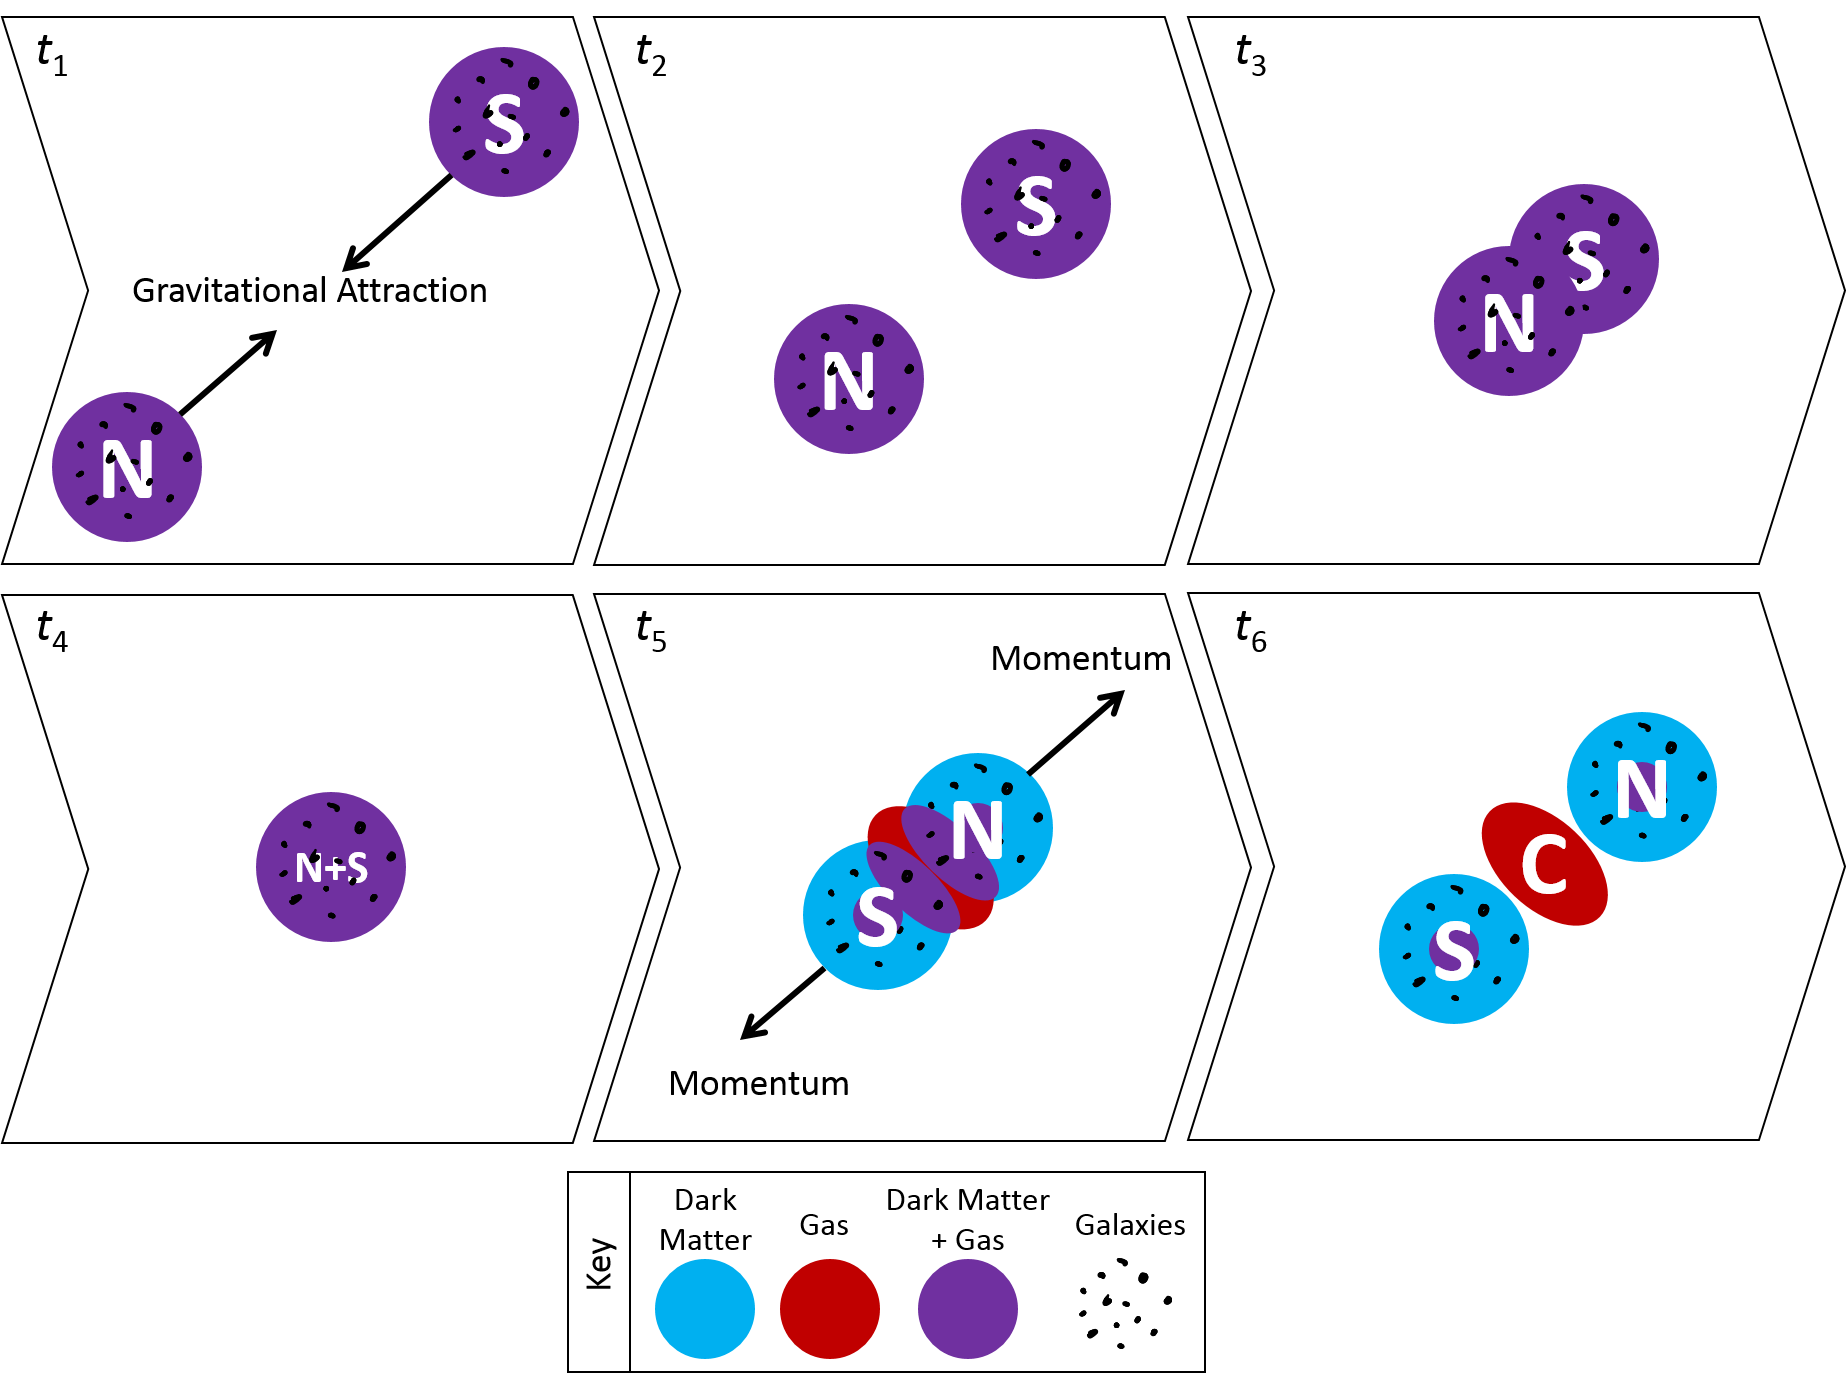
\includegraphics[width=6in]{Chapter1/MergerTimeSeries.png}
\caption{A basic time series leading to a dissociative galaxy cluster merger (assuming the Standard Model of Cosmology).
Two galaxy clusters (N \& S), each consisting of overlapping halos of DM and gas as well as sparsely populated galaxies, begin with an initial physical separation ($t_{\rm 1}$).
Due to the mass of each galaxy cluster they experience a gravitational attraction and accelerate towards one another until eventually they collide ($t_{\rm 1}$--$t_{\rm 4}$).
By convention time $t_{\rm 4}$ is defined as the ``collision''.
Because there is so much space between the galaxies, a strong interaction between any two galaxies is extremely unlikely and they can be treated as effectively collisionless particles.
And since the galaxies of each subcluster have built up momentum they will pass through and begin to separate (this time on the opposite side), $t_{\rm 5}$.
The gas however is more evenly distributed, thus an interaction between gas particles of each subcluster is more likely.
This interactions will convert some of the infall kinetic energy into thermal energy (i.e. the gas of each subcluster will experience ram pressure), the net effect being that the gas halo of each subcluster is slowed with respect to the galaxies and much of it becomes dissociated remains centered between the galaxies of the two subclusters ($t_{\rm 6}$ C).
Much like the galaxies the DM behaves in a nearly collisionless manner and appears largely coincident with the galaxies.
At $t_{\rm 6}$ the galaxy cluster merger is classed as \emph{dissociative merger}.
\label{fig:MergerTimeSeries}}
\end{figure}  

\subsection{Constraining Self-Interacting Dark Matter with Merging Galaxy Clusters}\label{section:DMconstraintWithMergers}

Think about moving some of the Figure \ref{fig:4ConstraintMethods} caption to the body text to make for a more concise caption.

\begin{figure}
\centering
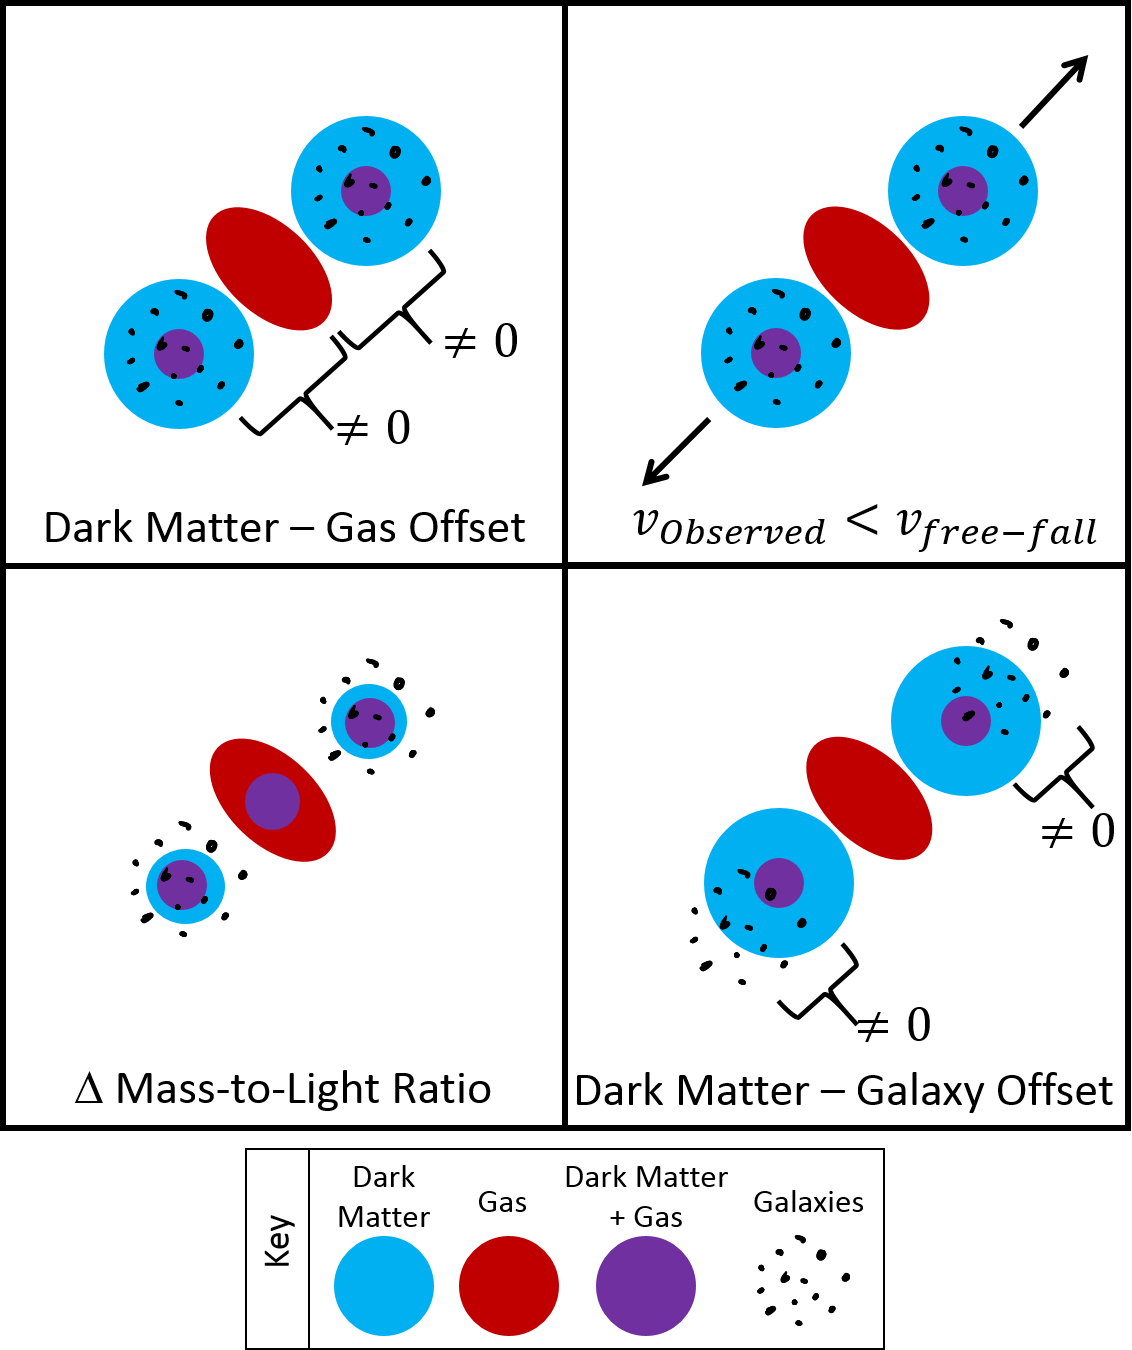
\includegraphics[width=4in]{Chapter1/4ConstraintMethods.png}
\caption{The four means of constraining $\sigma_{\rm SIDM}$ with merging clusters, originally outlined by \citet{Markevitch:2004dl} and \citet{Randall:2008hs}. 
\emph{Upper Left:} If the DM is significantly offset from the gas then the scattering depth of the dark matter ($\tau_{\rm DM}$) must be less than the scattering depth of the gas ($\tau_{\rm gas}$) and an upper limit can be placed on $\sigma_{\rm SIDM}$.
\emph{Upper Right:} If DM self-interacts during the merger, then the velocity of each subcluster will be slowed to some degree.
Thus if the observed velocity ($v_{\rm obs}$) is found to be consistent with the free-fall velocity ($v_{\rm free-fall}$) an upper limit can be placed on $\sigma_{\rm SIDM}$.
If however $v_{\rm obs}$ is significantly less than $v_{\rm free-fall}$, an upper limit could be potentially placed on $\sigma_{\rm SIDM}$.
\emph{Lower Left:} If DM self-interacts during the merger, then some fraction of the DM particles will scatter and become unbound from each subcluster.
Thus the mass-to-light ratio of each subcluster can be compared with the mass-to-light ratio of similar non-merging clusters, and depending on where the mass-to-light ratio of the merger is the same or less than the non-merging clusters' mass-to-light ratio, then respectively an upper limit or lower limit can be placed on $\sigma_{\rm SIDM}$.
\emph{Lower Right:} If the DM self-interacts during the merger, then the DM component of each subcluster will experience an additional drag force and will travel at a slower velocity than the respective subcluster galaxies.
Thus depending on whether a significant offset between the galaxies and DM is or is not observed, then respectively a lower limit or upper limit can be placed on $\sigma_{\rm SIDM}$.
\label{fig:4ConstraintMethods}}
\end{figure}

\subsection{Advantages of Merging Clusters Over other Probes of Self-interacting Dark Matter}

\section{Work Presented in this Dissertation}
Briefly summarize each chapter.

        % Either type your Introduction here or input a file 
        % containing it using the ``\input'' or ``\include'' command.
        
        % You will probably want to split your chapter up into several
        % sections (with each section possibly even split up into
        % subsections), each of which can either be written directly
        % in this file or input from an external file as above.
        %
        % Suggested sections for your introduction include a general 
        % overview (with historical motivation as appropriate) and a 
        % summary of your main results. E.g.:
        
    % %-----------------------------------------------------------------------
    % 
    % %-------------------------------------------------------- NEW CHAPTER --
    %
    % % -- Chapter 2


    \newchapter{Musket Ball: Observed Properties}{Musket Ball Cluster: Observed Properties}{Musket Ball Cluster: Observed Properties}
\label{chapter:2}

\noindent This chapter is an expanded version of the article titled \emph{Discovery of a Dissociative Galaxy Cluster Merger with Large Physical Separation} which was published in the March 2012 issue of the Astrophysical Journal Letters (Volume 747, pp. L42). \\

We present DLSCL J0916.2+2951 ($z$=0.53), a major cluster merger in which the collisional cluster gas has become dissociated from the collisionless galaxies and dark matter.
We identified the cluster using optical and weak lensing observations as part of the Deep Lens Survey. 
Our follow-up observations with {\it Keck}, {\it Subaru}, {\it Hubble Space Telescope}, and {\it Chandra} show that the cluster is a dissociative merger.


\section{Introduction}

We have identified a new dissociative merger, DLSCL J0916.2+2951, that probes an unexplored area of merger phase-space.  
We originally detected the cluster in the Deep Lens Survey \citep[DLS;][]{Wittman:2002cp} via its weak lensing (WL) shear signal. 
It consists of two main subclusters  spectroscopically confirmed to be at the same redshift (0.53).
This cluster was also observed in the Sunyaev-Zel'dovich Array Survey \citep{Muchovej:2010gc} which provided evidence that the cluster gas is dissociated from the bulk of the mass and galaxies (Figure \ref{figure:MusketBallSZ}).
Follow-up optical observations with {\it Subaru} and {\it HST} enable higher resolution mass maps and follow-up X-ray observations with {\it Chandra} ACIS-I confirm that the majority of the gas is offset between the North and South subclusters, the signature of a dissociative merger (Figure \ref{fig1}).

In this letter we introduce DLSCL J0916.2+2951 and summarize our survey of its three dominant components (galaxies, DM, and gas) and the cluster's astrophysical implications.
A more thorough exposition of the survey and analysis will be presented in Dawson et al. (in preparation).
Throughout this paper we assume $\Omega_{\Lambda}=0.7$, $\Omega_m=0.3$, and $H=70$\,km\,s$^{-1}$\,Mpc$^{-1}$.

\begin{figure}
\plotone{Chapter2/fig1.png}
\caption[Merging cluster DLSCL J0916.2+2951 and its three matter components.]{Merging cluster DLSCL J0916.2+2951 and its three matter components. 
Overlaid on the HST color image of the galaxies is the total mass distribution (blue) based on WL analysis of the HST images and the cluster gas distribution (red) based on Chandra X-ray observations.  
The bulk of the collisional gas is located between the two collisionless galaxy and mass concentrations, indicative of a dissociative merger. 
The image is $5\arcmin \times 5\arcmin$ ($\sim 1.9\times 1.9$\,Mpc$^2$ at $z=0.53$).\label{fig1}}
\end{figure}

\section{Photometric}

We obtained $B,V,R,$ and $z'$ photometric data (12, 12, 18, and 12\,ksec, respectively) with Mosaic 1 on the KPNO 4-m {\it Mayall} telescope as part of the DLS.
To improve the accuracy of our photometric redshifts we also observed the cluster in three medium-width optical bands ($g,h,$ and $i$ from the BATC filter set), bracketing the redshifted $4000$\,\AA\, feature, using the upgraded Mosaic 1.1 imager on the KPNO {\it Mayall} with exposure times of 6\,ks per filter (2011 April 22--24).
We estimate colors using \emph{ColorPro} \citep{Coe:2006jf} and redshifts using \emph{BPZ} \citep{Benitez:2000jr}.
We replace the standard templates with a set ``tweaked'' in a method similar to that described in \citet{Ilbert:2006bw}, using spectroscopic samples from SHELS \citep{Geller:2005dj} and the PRIMUS survey \citep{Coil:2010to} which overlap the DLS.
Figure \ref{fig2} shows the density isopleths of galaxies with $0.43<z_{\rm phot}<0.63$ (roughly the cluster redshift $\pm\sigma_{z_{\rm phot}}$).
This map agrees well with the distribution of spectroscopically confirmed cluster members.

\begin{figure}
%\epsscale{1.06}
\plottwo{Chapter2/fig2a.png}{Chapter2/fig2b.png}
\caption[Color image of DLSCL J0916.2+2951 and its galaxy number density with a histogram of the spectroscopic redshifts in the area.]{\emph{Left:} DLS composite $BVR$ color image of DLSCL J0916.2+2951 showing  the galaxies of the two subclusters. The white contours represent the number density of galaxies with $z_{\rm phot}=0.53\pm0.1$, the cluster redshift $\pm\sigma_{z_{\rm phot}}$. The contours begin at 200 galaxies\,Mpc$^{-2}$ with increments of 50 galaxies\,Mpc$^{-2}$. 
The image field-of-view is the same as Figure \ref{fig1}.
\emph{Right:} Histogram of the 200 observed spectroscopic redshifts within the field of view of the \emph{left} figure.  The red portion is the subsample that passes the $z_{\rm phot}=0.53\pm0.1$ criteria. The galaxies at $z\sim0.6$ had equal probability of selection as the cluster members and show no sign of clustering. 
\label{fig2}}
\end{figure}

\section{Spectroscopic}\label{section:MusketBallSpectroscopy}

We obtained spectroscopic redshifts for 20 cluster members with {\it Keck} LRIS (2007 January 16) and 634 unique spectroscopic redshifts (0\,$<$\,$z$\,$<$\,1.2)  in a $\sim15\arcmin\times 15\arcmin$ area centered on the cluster with {\it Keck} DEIMOS (2011 March 2--3), including 132 members at the cluster redshift.
We reduced the LRIS spectra using a scripted sequence of standard IRAF reduction tasks, and the DEIMOS spectra using a modified version of the DEEP2 \emph{spec2d} package \citep{Davis:2003fe,Gal:2008bg,Lemaux:2009fy}.

We use our full sample of 654 spectroscopic redshifts as well as photometric redshifts to identify potential line-of-sight structures which may confuse our results.
We find no evidence for significant line-of-sight structure (Figure \ref{fig2}).

We estimate each subcluster's redshift and velocity dispersion (Table \ref{tbl1}) using the biweight-statistic and bias-corrected 68\% confidence limit \citep{Beers:1990kg} applied to 100,000 bootstrap samples of each subcluster's spectroscopic redshifts.
Our redshift estimates indicate a line-of-sight velocity difference of $v_{\rm los}=670^{+270}_{-330}$ km s$^{-1}$ between the North and South subclusters, using the galaxies within a 0.5\,Mpc radius centered on the {\it HST} WL mass peaks and within a velocity range of $\pm 3000$\,km\,s$^{-1}$ of $z$=0.53 ($\sim3\times$ the expected velocity dispersion); corresponding to 38 and 35 galaxies for the North and South subcusters, respectively.
These results are robust against varying the velocity range $\pm1000$\,km\,s$^{-1}$ and using the Subaru WL or galaxy number density peaks as the apertures' centers, provided the aperture radius is $\lesssim$0.5\,Mpc: larger radii lead to significant subcluster membership confusion.
Additionally, we report the velocity dispersion mass estimates based on the scaling relation of \citet{Evrard:2008jm} in Table \ref{tbl1}.
We note that the velocity dispersions should be interpreted with caution since this is a disturbed system.

\begin{deluxetable}{lcccccccc}
\tablewidth{0pt}
\tabletypesize{\scriptsize}
\tablecaption{Observed subcluster and X-ray concentration properties\label{tbl1}}

\tablehead{
\colhead{Subcluster}     & \colhead{Redshift}  &
 \colhead{$\sigma_v$}    &  \colhead{$\sigma_v$ M$_{200}$}&
\colhead{WL M$_{200}$}          &
\colhead{L$_{\rm X_{\rm 0.5-2keV}}$}  & \colhead{T$_{\rm X}$}  &
\colhead{X-ray} & \colhead{Joint WL}\\
\colhead{}         &  \colhead{}  &
\colhead{(km s$^{-1}$)}    &   \colhead{($10^{14}$M$_\sun$)}  & 
\colhead{($10^{14}$M$_\sun$)}          &
\colhead{($10^{43}$erg\,s$^{-1}$)}  & \colhead{(keV)}  &
\colhead{S/N} & \colhead{S/N} 
}
\startdata
North & $0.53074^{+0.00068}_{-0.00064}$ & 
 $740^{+130}_{-190}$ &
 $3.7\pm2.3$& $1.7^{+2.0}_{-0.72}$ &
0.63 & \nodata &
 3.2 & 3.0 \\
South  & $0.53414^{+0.00065}_{-0.00064}$ & 
 $770^{+110}_{-92}$ & 
 $4.1\pm1.6$& $3.1^{+1.2}_{-0.79}$ &
2.1 & $2.7^{+1.2}_{-0.7}$ &
7.0 & 6.7\\
Central & \nodata & 
\nodata & \nodata & 
\nodata &
2.8 & $2.2^{+1.4}_{-0.6}$ &
9.1 & -3.3\tablenotemark{a}\\ 
\enddata
%% Text for table notes should follow after the \enddata but before
%% the \end{deluxetable}. Make sure there is at least one \tablenotemark
%% in the table for each \tablenotetext.
\tablenotetext{a}{The negative WL S/N indicates a projected surface mass local under-density.}
%\tablecomments{Table \ref{tbl-1} is published in its entirety in the 
%electronic edition of the {\it Astrophysical Journal}.  A portion is 
%shown here for guidance regarding its form and content.}
%\tablenotetext{a}{Sample footnote for table~\ref{tbl-1} that was generated
%with the deluxetable environment}
%\tablenotetext{b}{Another sample footnote for table~\ref{tbl-1}}
\end{deluxetable}

\section{Weak Lensing}

To map the total mass distribution we use a version of the \citet{Fischer:1997ct} method modified to include a novel tomographic signal-matched filter.
The cluster's WL shear signal, $\gamma$, depends not only on the projected surface mass over-density of the cluster, $\Delta\Sigma$, but on the relative distances of the observer, the mass, and the background galaxies:
\begin{displaymath}
\gamma=\frac{\Delta\Sigma}{\Sigma_{cr}}=\frac{\Delta\Sigma4\pi G}{c^2}\frac{D_{ls}(z_l,z_s)D_l(z_l)}{D_s(z_s)}\mathcal{H}\left(\frac{z_s}{z_l}-1\right),
\end{displaymath}
%\begin{displaymath}
%\gamma \propto \frac{\Delta\Sigma}{\Sigma_{cr}} = \Delta\Sigma \frac{4\pi G}{c^2} \frac{D_{ls}(z_l,z_s)D_l(z_l)}{D_s(z_s)} \mathcal{H}\left(\frac{z_s}{z_l}-1\right),
%\end{displaymath}
where $\Sigma_{\rm cr}$ is the critical surface density, $\mathcal{H}$ is the Heaviside step function,  and $D_l$, $D_s$, \& $D_{ls}$ are the angular diameter distances to the lens, source, and between the lens and source, respectively.
Since we do not have exact redshift measurements of the source galaxies we use each galaxy's photometric redshift probability distribution function, $p(z)$, to estimate a respective $\Sigma_{\rm cr}$ for a given lens redshift,
\begin{displaymath}
\Sigma_{cr}(z_l)\approx\langle\Sigma_{cr}(z_l)\rangle=\int\Sigma_{cr}( z_l,z_s)p(z_s)dz_s.
\end{displaymath}
In addition to weights based on shape measurement errors, we also weight the shear of each galaxy based on its $p(z)$,
\begin{displaymath}
w_{\gamma}(z_l)=\frac{1}{\int\left[\Sigma_{cr}(z_l,z_s)-\langle\Sigma_{cr}(z_l)\rangle\right]^2p(z_s)dz_s}.
\end{displaymath}
%\begin{displaymath}
%w_{\gamma}(z_l)=\frac{1}{\sigma^2_{\Sigma_{cr}}}=\frac{1}{\int\left[\Sigma_{cr}(z_l,z_s)-\langle\Sigma_{cr}(z_l)\rangle\right]^2p(z_s)dz_s}.
%\end{displaymath}
This method increases the signal-to-noise of the measurement \citep[see e.g.][]{Hennawi:2005ig}, and more accurately accounts for the errors inherent in the photometric redshift estimates, compared to single-point estimates.
We estimate uncertainties using 100 bootstrap resamplings.

Encouraged by the DLS mass and galaxy maps we obtained higher-resolution ground and space based observations.
{\it Subaru} Suprime-Cam $i'$-band coverage of the cluster was provided by engineering-time observations of DLS Field 2 (2008 January 8).
We use the Suprime-Cam data reduction software \emph{SDFRED} \citep{Yagi:2002ed,Ouchi:2004da} followed by \emph{SCAMP} \& \emph{SWARP} \citep{Bertin:2002wn,Bertin:2006vk} to refine the astrometry and make the final mosaic. 
DLSCL J0916.2+2951 was also observed with {\it HST} ACS/WFC using F606W and F814W filters (GO-12377, PI-W. Dawson) in a $2\times1$ pointing mosaic that covers the subclusters (Figure \ref{fig1}). 
The exposure times for F606W and F814W are 2520s and 4947s per pointing, respectively.  
We reduce this data following a method similar to that presented in \citet{Jee:2009cr}.  
We measure the PSF of both datasets using the PCA method presented in \citet{Jee:2007bq}.

We perform our WL analysis independently on both the Subaru and HST F814W data. The Subaru data has $0.72\arcsec$ seeing and 49 WL-quality source galaxies (i.e.\,background galaxies with measured ellipticity error  $<0.3$) per arcmin$^2$. For the mass map we use an apodizing kernel radius of $0.5\arcmin$, which can be interpreted as the effective resolution of the WL mass map.
We are able to cross-match most of the detected objects with the DLS and use the $p(z)$'s discussed in the previous section.

Cross-matching is more problematic with the higher-resolution HST data, so we use a color-magnitude cut (F606W-F814W\,$<$\,0.8 and 24\,$<$\,F814W\,$<$\,28.5) to select source galaxies and exclude cluster red-sequence and bright foreground galaxies, see Figure \ref{figure:HSTcolormag}.
For the WL analysis of the HST F814W image, which has a $0.1\arcsec$ PSF and 136 WL-quality source galaxies per arcmin$^{2}$, we use an  apodizing kernel radius of $3.6\arcsec$.
We find no significant spatial correlation between source density and subcluster position, suggesting that our source galaxy population is not significantly contaminated with cluster galaxies.
Furthermore, we find a comparable number distribution of sources as a function of magnitude when we make similar cuts to the HUDF \citep{Coe:2006jf} and GOODS North \& South \citep{Giavalisco:2004kl} galaxy catalogs, indicating negligible cluster contamination, see Figure \ref{figure:HSTsourcedensity}.
We estimate the $p(z)$ of our HST source galaxy sample by assuming the photometric redshift distribution of the \citet{Coe:2006jf} HUDF catalog after applying our color-magnitude cut.
Figure \ref{fig3} shows excellent agreement between the Subaru and HST WL mass, and galaxy density maps.

\begin{figure}
\centering
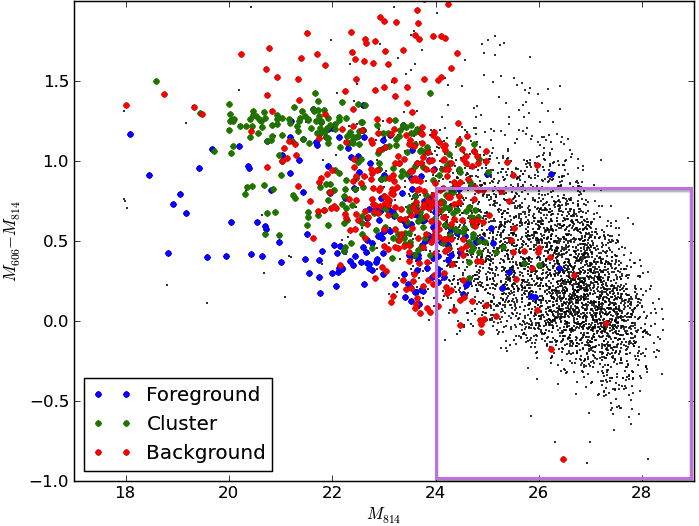
\includegraphics[width=4in]{Chapter2/HSTcolormag_wBPZ.png}
\caption[Musket Ball Cluster color-magnitude diagram based on HST photometry, along with galaxy location based on DLS photometric redshifts.]{Musket Ball Cluster color-magnitude diagram based on HST photometry.  The larger color points are cross-matched DLS objects which have been divided into \emph{Foreground} (blue; $z_{\rm phot}<0.43$), \emph{Cluster} (green; $z_{\rm phot}=0.53\pm0.1$), and \emph{Background} (red; $z_{\rm phot}>0.63$) samples.  Note that the photometric redshifts become relatively unreliable for $M_{\rm 814}>24$. 
The purple box indicates the HST source galaxy sample.  
\label{figure:HSTcolormag}}
\end{figure}

\begin{figure}
\centering
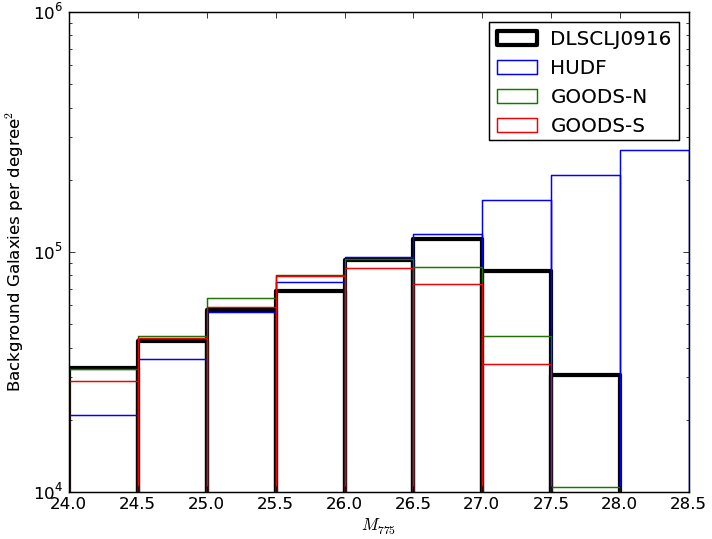
\includegraphics[width=4in]{Chapter2/UDF_GOODS_sourcemaghist.png}
\caption[Comparison of the Musket Ball Cluster, HUDF and GOODS North \& South source galaxy densities.]{Comparison of the Musket Ball Cluster, HUDF \citep{Coe:2006jf} and GOODS North \& South \citep{Giavalisco:2004kl} source galaxy densities.
The HUDF field has a depth of 288 F775W orbits, the GOODS survey has a depth of one F775W orbit, and the Musket Ball Cluster has a depth of 2 F814W orbits (the F814W filter is comparable to the F775W filter).
Up to the completeness of each survey we find a comparable number distribution of sources as a function of magnitude when we make similar cuts to each galaxy catalog, indicating negligible cluster contamination.
\label{figure:HSTsourcedensity}}
\end{figure}

We construct a joint catalog from the HST and Subaru data, using the HST data where available and Subaru for the surrounding area.
Using a tomography-based MCMC analysis we simultaneously fit NFW halos centered on the North and South HST WL peaks, and use the \citet{Gelman:1992ht} convergence test applied to eight independent chains.
In order to reduce the number of free parameters we use the \citet{Duffy:2008jy} empirical relation between $M_{200}$ and concentration.
We present the most likely masses for each halo along with the bias-corrected 68\% confidence limits in Table \ref{tbl1}.
We also compare the integrated projected surface mass density of the NFW halos with the measured WL aperture mass \citep{Fahlman:1994eb} of each subcluster and find agreement within a radius of 0.5 Mpc of each subcluster.

\begin{figure}
%\plottwo{fig3a.eps}{fig3b.eps}
\plotone{Chapter2/fig3.png}
\caption[Comparison of the Subaru $i'$-band ground-based and HST space-based  WL mass signal-to-noise maps of DLSCL J0916.2+2951 with the X-ray distribution and galaxy number density.]{Comparison of the Subaru $i'$-band ground-based (left) and HST space-based (right) WL mass signal-to-noise maps (color) of DLSCL J0916.2+2951 with the X-ray distribution (bold black contours) and galaxy number density (white contours, same as Figure \ref{fig2}). The peak centers and corresponding one sigma errors are denoted by the gray cross-hairs.
In both analyses there is agreement between the location and relative magnitude of galaxies and WL yet the majority of the cluster gas is centered $\sim1.4\arcmin$ between the North and South subclusters in a local mass underdensity, providing evidence that the North and South subclusters have undergone the first pass-through of a major merger.
The scale of each map is equivalent and the image field-of-view is the same as Figures \ref{fig1} \& \ref{fig2}.
The map created from the joint Subaru/HST catalog looks nearly identical to the HST map, with only slight variations in the scale (see Table \ref{tbl1}).
\label{fig3}}
\end{figure}

\section{Sunyaev--Zel'dovich Effect}

This cluster was also observed in the Sunyaev-Zel'dovich Array Survey \citep{Muchovej:2010gc}.  
They found a 4{$\sigma$} SZE signal roughly consistent with that expected for clusters of this mass.
The signal is offset $\sim$ 1' ($\sim$ 0.4 Mpc) from the southern subcluster and $\sim$ 3' ($\sim$ 1 Mpc) from the northern subcluster.
The SZE traces the cluster ICM and can be used to identify an offset of the ICM relative to the galaxies and dark matter \citep[as in the case of the Bullet Cluster][]{Halverson:2009gn}.
This shift provided the first evidence that the cluster gas is dissociated from the bulk of the mass and galaxies (Figure \ref{figure:MusketBallSZ}).

\begin{figure}
\centering
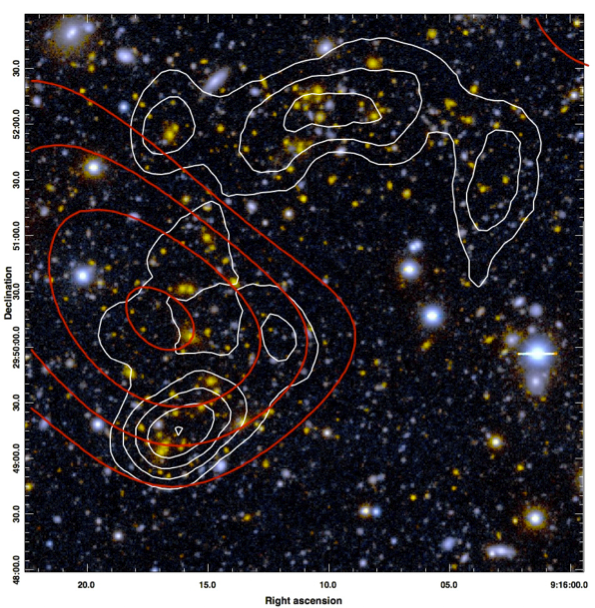
\includegraphics[width=4in]{Chapter2/color_2contours_noblue_edit.png}
\caption[DLS optical image with SZE and galaxy number density maps.]{DLS composite $BVR$ color image of DLSCL J0916.2+2951 showing evidence that the cluster gas, represented by the solid red SZE decrement significance contours (1, 2, 3, 4$\sigma$), is offset $\sim1\arcmin$ ($\sim0.4$ Mpc) and $\sim3\arcmin$ ($\sim1$ Mpc) from the two subclusters, represented by the white galaxy number density contours for galaxies with $z_{\rm phot}=0.53\pm0.1$ (beginning at 200 galaxies\,Mpc$^{-2}$ with increments of 50). 
The image field-of-view is the same as Figure \ref{fig1}. 
The beam of the SZ observation has a radius of $\sim1\arcmin$.\label{figure:MusketBallSZ}}
\end{figure}

\section{X-ray}

We acquired X-ray spectral-imaging of the cluster with 40ks of {\it Chandra} ACIS-I time (GO-12800854), and reduce it using \emph{CIAO} version 4.2 and \emph{CALDB} version 4.4.1.
We manually identify X-ray point sources and mask them before adaptively smoothing the diffuse emission, we present the resulting map in Figure \ref{figure:MusketBallXray}.
We estimate source counts and their error using the \emph{dmextract} function of \emph{CIAO}.
We use an 8$\arcmin$ radius background region which encloses the subcluster regions and rests $\sim90\%$ on ACIS-I3 (on which the subclusters are observed).
In the estimate of the background counts each subcluster region, chip gap, and point source are excluded.
The subcluster exclusion regions were defined such that they encompassed the source emission and were extended out to approximately the SNR = 1 level based on the smoothed map.
In total we there were $1800\pm40$ background counts in 620,000 pixel$^2$ area within the energy range of 0.5-2\,keV.
For the South and Central X-ray concentrations (120$\pm$17 and 170$\pm$19 detected 0.5-2\,keV photons, respectively) we use the \emph{Xspec} X-ray spectral fitting tool \citep{Arnaud:1996vl} to fit a Mewe-Kaastra-Liedahl plus photoelectric absorption model \citep[fixed to the Leiden/Argentine/Bonn value;][]{Kalberla:2005de} to the X-ray spectrum of each X-ray concentration.
For the North concentration there are not enough detected X-ray photons (38$\pm$12) to fit a meaningful spectrum.  
We report the results of this analysis in Table \ref{tbl1}. 
We define the subcluster exclusion regions such that they encompass the source emission and extend out to approximately the 1$\sigma$ level based on the smoothed map.  
In total there are $1800\pm40$ background counts in the 620,000\,pixel$^2$ area and 0.5-2\,keV energy range.
For the North, South, and Central X-ray concentrations we find 38$\pm$12, 120$\pm$17 and 170$\pm$19 detected 0.5-2\,keV photons, respectively.   
 
To estimate the temperatures of the South and Central concentrations we use the \emph{Xspec} X-ray spectral fitting tool \citep{Arnaud:1996vl} to fit a Mewe-Kaastra-Liedahl plus photoelectric absorption model \citep[fixed to the Leiden/Argentine/Bonn value;][]{Kalberla:2005de} to the X-ray spectrum of each X-ray concentration.  
For the North concentration there are not enough detected X-ray photons to fit a meaningful spectrum.  
Due to the low count regime and our use of the $\chi^2$ statistic we rebin the data so that each spectral channel used in the fit contains at least 20 counts.
The binning is carried out on the spectra before background subtraction; these raw spectra contained 843 (1070) counts in the South (Central) subcluster.
Since the background spectrum contains 7725 counts, each spectral bin in the background is far above the 20 count threshold.
Binning data in this manner does reduce the spectral resolution, however for hot clusters like those in our study the number of final spectral bins we have (31 for the southern and 39 for the central subcluster, which include cuts on the highest energy channels) are sufficient to determine the temperature, since the spectrum is dominated by bremsstrahlung emission which has few sharp spectral features. 
We report the results of this analysis in Table \ref{tbl1}.

\begin{figure}
\centering
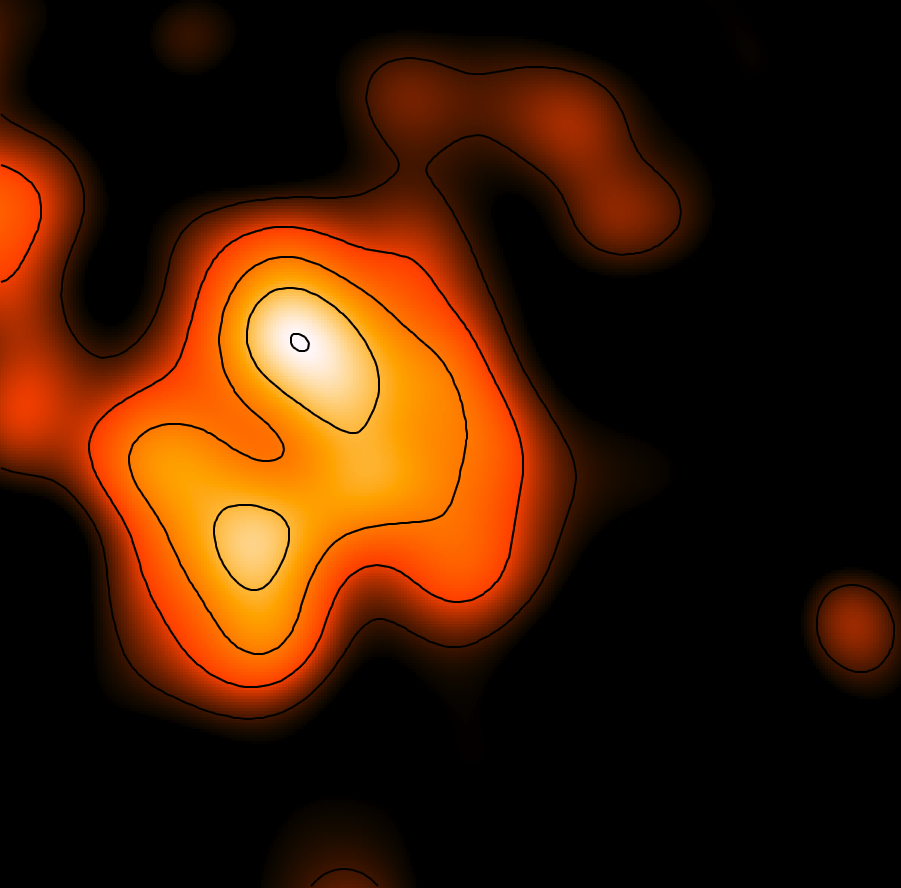
\includegraphics[width=4in]{Chapter2/XrayMapwithContours.png}
\caption[X-ray map of the Musket Ball Cluster]{
Chandra ACIS-I 40\,ks adaptively smoothed X-ray image of DLSCL J0916.2+2951.
The image field-of-view is the same as Figure \ref{fig1}.
The contours are evenly spaced on an arbitrary linear scale and are used throughout this dissertation when comparing the gas map with other components.
\label{figure:MusketBallXray}}
\end{figure}

\section{Radio}

Since the Musket Ball cluster is a strong merger with an X-ray inferred Mach number of > 3 whose axis is likely to be close to the plane of the sky \citep{Dawson:2012ub}, it is a prime candidate for a double radio relic. 
Radio relics are irregularly shaped radio sources, located at the outskirts of galaxy clusters, characterized by steep radio spectrum\footnote{The spectrum is defined as $S(/nu)\propto\nu^\alpha$.} with $\alpha\leq -1.2$.
Radio relics are thought to be produced by relativistic particles that have been accelerated by shock waves in the ICM.
Double relics show relics on opposite sides from the cluster center and form a subset of relics for which the merger geometry can be constrained particularly well \citep[see e.g.][]{Bonafede:2012fu}.

Since the Musket Ball Cluster is at a later stage than all other dissociative
mergers \citep{Dawson:2012dl} and is thought to have shocks with $M >
3$, the detection of radio relics would provide constraints on the merger geometry. 
This has direct implications for the measurement of the dark matter cross-section with the Musket Ball since observed projected offsets must be translated into meaningful physical offsets \citep[see e.g.][]{Dawson:2012ub}. 
The degree of polarization provides important information on the angle of the shock surface and the line of sight and together with the location of the relics with respect to the X-ray position we can constrain the geometry of the merger axis to within 10 degrees \citep{vanWeeren:2011cd}. 
Furthermore, the cluster makes an ideal target to study the evolution of radio relics, due to its superior temporal lever arm, with ramifications for the theory of particle acceleration. 

The Musket Ball Cluster is located at $z$ = 0.53 and at this redshift a typical moderate luminosity radio relic has a flux density of 0.3 mJy at $z$ = 0.53 and 1.4 GHz \citep{Nuza:2012fu, vanWeeren:2011cd}. 
This is well below both the NRAO VLA Sky Survey (NVSS) and Westerbork Northern Sky Survey (WENNS) sensitivities, thus an existing non-detection in these surveys is not surprising. 

We observed the Musket Ball Cluster with the Westerbork Synthesis Radio Telescope (WSRT) in 2013 January 23-28 for a total of 24 hours.  We used the standard 21\,cm L-band as it is the most sensitive system at the WSRT.
The observations have a resolution of about 15x30 arcsec, corresponding to a physical size of 100x200kpc at z = 0:53, enough to resolve a 1 Mpc relic (relic sizes range between 0.5 and 2 Mpc).
With two full synthesis runs we achieved a noise level of 20\,$\mu$Jy/beam in the continuum, and about 10\,$mu$Jy/beam in Stokes Q and U. 
This should enable us to detect a 0.3\,mJy relic, covering 5 beam areas, with
an SNR of 10. 

While there are a number of compact sources associated with the merging cluster (see the $X$'s in Figure \ref{figure:MusketBallRadio}), we find no evidence for diffuse radio emission associated with the merging cluster.
In other words, no radio halos or relics are detected in the Musket Ball Cluster merger.
All previously discovered radio relics have been in clusters with X-ray luminosities in the range of 10$^{44}$-10$^{45}$\,erg\,s$^{-1}$.
The Musket Ball Cluster has an X-ray luminosity of $\sim 10^{43}$\,erg\,s$^{-1}$ (see Table \ref{tbl1}). 
This null detection is in line with the current trend that radio relics are only found in very massive cluster mergers.

\begin{figure}
\centering
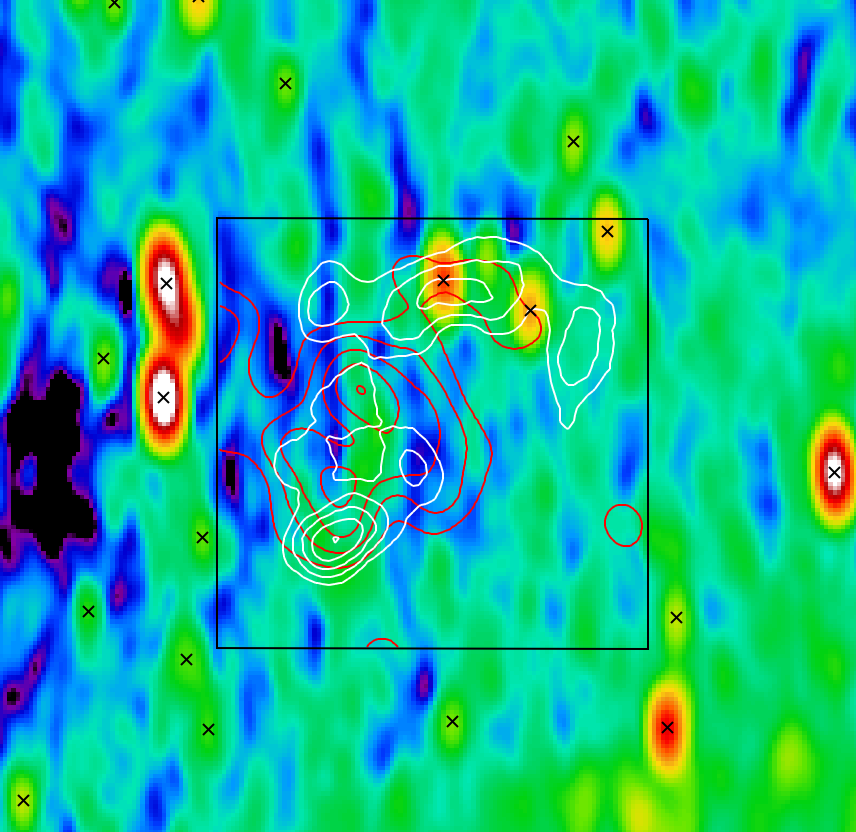
\includegraphics[width=4in]{Chapter2/RadioWithGalaxyAndXrayContours.png}
\caption[Radio survey of the Musket Ball Cluster and surrounding area.]{
Westerbork Synthesis Radio Telescope 21cm L-band image of the Musket Ball Cluster and surrounding area.  The color image has an arbitrary log-scale.  Likely compact radio sources are denoted by the \emph{X} points, and from these the north/south elongated PSF can be seen.  The black box shows the area corresponding to Figures \ref{fig1}, \ref{fig2}, and \ref{fig3}. Similarly the white contours are the galaxy number density contours from Figure \ref{fig2}, and the red contours are the X-ray contours from Figure \ref{fig3}.  We detect no significant diffuse radio emission associated with the Musket Ball Cluster (i.e. no radio halos or relics are detected).
\label{figure:MusketBallRadio}}
\end{figure}

\section{Cluster Merger Scenario}

The peak of the gas distribution ($09\fh16\fm15\fs\pm5.5\fs, 29\fdg50\farcm59\farcs\pm5.0\farcs$) derived from X-rays is offset $1.4\arcmin\pm0.49$ from the North HST WL mass peak ($09\fh16\fm10\fs\pm30\fs, 29\fdg52\farcm10\farcs\pm30\farcs$), and $1.4\arcmin\pm0.14$ from the South HST WL mass peak ($09\fh16\fm15\fs\pm8.0\fs, 29\fdg49\farcm34\farcs\pm6.9\farcs$), and is located near a local minimum in the mass, suggesting that the subclusters have a small impact parameter and have experienced at least their first pass-through along a north-northwest merger direction (see Figure \ref{fig3}).
Additionally the Central X-ray concentration has a temperature (Table \ref{tbl1}) in line with an M$_{500}=0.9^{+1.1}_{-0.3}\times10^{14}$\,M$_{\odot}$ potential \citep{Vikhlinin:2009jy}, but the WL data suggests that there is a local under-density of mass at this concentration incapable of supporting such a temperature.
Further evidence for the merger scenario is provided by the morphology of the gas.
Simulations \citep{Schindler:1993vl,Poole:2006gp} predict that the gas morphology elongates transverse to the merger direction after pass-through for mergers with small impact parameters.
The Central gas concentration appears to be oblate and roughly perpendicular to the axis connecting the North and South mass peaks.
This is consistent with the interpretation that these two subclusters have experienced their first pass-through and that the merger axis being roughly in the plane of the sky.

\section{Discussion}

While we use DLSCL J0916.2+2951 to provide further evidence for the canonical DM model and independently constrain $\sigma_{\rm DM}m^{-1}_{\rm DM}$, we believe that its greatest value is as a probe for a new and special phase of cluster formation.  
It provides a greatly improved temporal lever-arm with which to guide numerical simulations that explore the major merger phase.  
This is potentially important given that much of our knowledge of the cluster merger process comes from numerical hydrodynamic simulations \cite[e.g.][]{Poole:2006gp}, which are used to place the tightest constraints on $\sigma_{\rm DM}m^{-1}_{\rm DM}$ \citep[$<0.7$\,cm$^2$\,g$^{-1}$;][]{Randall:2008hs} and bring observed merger velocities (inferred from the observed shock velocity) more in line with the expectations of $\Lambda$CDM \citep{Springel:2007bg,Lee:2010id}.
Secondly, the large projected separation relative to the virial radii of the subclusters ($R_{200} \sim 1$Mpc) enables the deconvolution of the subclusters from the Central region and direct comparison of the physical properties of each.
This will provide new insight into the behavior of the cluster constituents (gas, galaxies, \& DM) during a major merger.
For example, it is well established that galaxy clusters play an important role in the evolution of their member galaxies, but it is still unclear whether cluster mergers trigger star formation \citep[e.g.][]{Miller:2003kx,Owen:2005dx,Ferrari:2005es,Hwang:2009ip}, quench it \citep{Poggianti:2004ca}, or have no immediate effect \citep{Chung:2010ds}.

Our identification of DLSCL J0916.2+2951 as a dissociative merging system using only optical, WL, and SZE observations shows that these systems can be found independent of X-ray observations.
This has implications for finding more of these systems when the existing SZE surveys, e.g. ACT \citep{Hincks:2010ff} and SPT \citep{Ruhl:2004io}, are coupled with upcoming and overlapping deep optical/WL surveys, e.g. DES \citep{Collaboration:2005vv} and LSST \citep{Tyson:2002hn}.

\section{Conclusions}

Conclusion text

\textbf{acknowledgements:}

We thank Daniel P. Marrone, Stephen Muchovej,  John E. Carlstrom, and Tony Mroczkowski of the SZA collaboration for sharing the results of the SZA Survey, which helped motivate the detailed follow-up campaign of DLSCL J0916.2+2951. 
Support for this work was provided by NASA through Chandra Award Number GO1-12171X issued by CXO Center, which is operated by the SAO for and on behalf of NASA under contract NAS8-03060.  Support for program number GO-12377 was provided by NASA through a grant from STScI, which is operated by the Association of Universities for Research in Astronomy, Inc., under NASA contract NAS5-26555.

This work made use of the following facilities: CXO (ACIS-I), HST (ACS), Keck:I (LRIS), Keck:2 (DEIMOS), Mayall (MOSAIC 1 \& 1.1), Subaru (Suprime-Cam), SZA.


    % %-----------------------------------------------------------------------
    % 
    % %-------------------------------------------------------- NEW CHAPTER --
    %
    % % -- Chapter 3

    \newchapter{Dynamics of Merging Clusters}{Dynamics of Merging Clusters}{The Dynamics of Merging Clusters:\\
		A Monte Carlo Solution Applied to the Bullet and Musket Bal}
\label{ch3}

\noindent This chapter was originally published as an article with the same
title in the June 2010 issue of the Astrophysical Journal Letters
(Volume 716, Number 2, pp. L185-L189). \\

Merging galaxy clusters have become one of the most important probes of dark matter, providing evidence for dark matter over modified gravity and even constraints on the dark matter self-interaction cross-section.  
To properly constrain the dark matter cross-section it is necessary to understand the dynamics of the merger, as the inferred cross-section is a function of both the velocity of the collision and the observed time since collision.
While the best understanding of merging system dynamics comes from N-body simulations, these are computationally intensive and often explore only a limited volume of the merger phase space allowed by observed parameter uncertainty.  
Simple analytic models exist but the assumptions of these methods invalidate their results near the collision time, plus error propagation of the highly correlated merger parameters is unfeasible.
To address these weaknesses I develop a Monte Carlo method to discern the properties of \emph{dissociative mergers} and propagate the uncertainty of the measured cluster parameters in an accurate and Bayesian manner.
I introduce this method, verify it against an existing hydrodynamic N-body simulation, and apply it to two known dissociative mergers: 1ES 0657-558 (Bullet Cluster) and DLSCL J0916.2+2951 (Musket Ball Cluster).
I find that this method surpasses existing analytic models --- providing accurate (10\% level) dynamic parameter and uncertainty estimates throughout the merger history.
This coupled with minimal required \emph{a priori} information (subcluster mass, redshift, and projected separation) and relatively fast computation ($\sim$6 CPU\,hours) makes this method ideal for large samples of dissociative merging clusters.

\section{Introduction}\label{sec_intro}
% %%% Context
Merging galaxy clusters have become important astrophysical probes providing constraints on the dark matter (DM) self-interaction cross-section \citep[$\sigma_{\rm DM}$;][]{Markevitch:2004dl, Randall:2008hs, Merten:2011gu, Dawson:2012dl}, and the large-scale matter-antimatter ratio \citep{Steigman:2008dy}.
They are a suspected source of extremely energetic cosmic rays \citep{vanWeeren:2010dn}, and the merger event potentially affects the evolution of the cluster galaxies \citep[e.g.][]{Poggianti:2004ca,Hwang:2009ip,Chung:2009bz}.
All of the respective astrophysical conclusions drawn from merging clusters depend on the specific dynamic properties of a given merger.

%%%% Need

For example, the subclass of dissociative mergers, in which the collisional cluster gas has become dissociated from the near collisionless galaxies and dark matter,  provides four ways of constraining the dark matter self-interaction cross-section \citep{Markevitch:2004dl,Randall:2008hs}.
The best constraints come from studying the mass-to-light ratios ($M/L$) of the subclusters\footnote{I define \emph{subcluster} as either one of the two colliding clusters, irrespective of mass, and I define \emph{cluster} as the whole two-subcluster system.}, and the offset between the collisionless galaxies and dark matter \citep{Markevitch:2004dl,Randall:2008hs}.
Both constraints directly depend on the merger dynamics.
First the relative collision velocity will affect the expected momentum transfer between each subcluster's dark matter particles which will in turn affect the expected dark matter mass transfer from the smaller subcluster to the larger subcluster ultimately affecting the expected mass to light ratios of the clusters \citep{Markevitch:2004dl}.
Second the expected galaxy--dark matter offset will depend on the observed time-since-collision\footnote{I define the time of collision to be the time of the first pericentric passage.} ($TSC$).
Initially the offset between the galaxies and dark matter will increase with $TSC$ (for $\sigma_{\rm DM} > 0$) as the collisionless galaxies outrun the dark matter that experienced a drag force during the collision, then at later $TSC$ the offset will decrease due to the gravitational attraction between the galaxies and dark matter halo. 
Additionally it is important to know the velocity so that dark matter candidates with velocity dependent cross-sections \citep[e.g.][]{Colin:2002ku,Vogelsberger:2012dy} can be constrained.

However there is no way to directly observe the dynamic merger parameters of principal interest: the three-dimensional relative velocity ($v_{\rm 3D}$) and separation ($d_{\rm 3D}$) of the subclusters as a function of time, their maximum separation ($d_{\rm max}$), the period between collisions ($T$), and the time-since-collision ($TSC$).
Observations are generally limited to: the subcluster projected separation ($d_{\rm proj}$), the line-of-sight (LOS) velocity of each subcluster ($v_i$) as inferred from their redshifts, and their mass ($M_i$) or projected surface mass density profile.
In addition to the obvious inability to measure a change in the merger state, it is difficult to constrain the dynamic parameters of interest even in the observed state. 
This is due to the general inability to constrain the angle of the merger axis with respect to the plane of the sky ($\alpha$), see Figure \ref{fig_mergerdiagram}.

For the Bullet Cluster it was originally thought that estimates of the Mach number of the cluster merger through X-ray observations of the gas shock feature \citep[e.g.][]{Markevitch:2006wv} could be used to estimate $v_{\rm 3D}$, and in conjunction with measurements of the relative LOS velocities then estimate $\alpha$.
Similarly, the gas pressure differential across cold front features seen in some merging clusters have also been used to estimate the Mach number of the cluster merger \citep[e.g.][]{Vikhlinin:2003wy}. 
However, \citet{Springel:2007bg} showed that the Mach number only translates to an upper limit on $v_{\rm 3D}$, and in the case of the Bullet Cluster they showed that the Mach inferred velocity could be a factor of $\sim2$ larger than the true $v_{\rm 3D}$.
There is potential for constraining $\alpha$ using polarization measurements of radio relics \citep{Ensslin:1998tx}, which are associated with some cluster mergers \citep[e.g.\,][]{vanWeeren:2010dn} but not all \citep[e.g.\,][]{Russell:2011hn}. 
Even if for some mergers radio relics provide constraints on $\alpha$, dynamic models are still needed in order to ascertain the dynamic properties of the merger throughout time.

The two most prevalent methods for ascertaining the dynamics of observed merging systems are \emph{the timing argument} and N-body simulations.  
The timing argument is based on the solution to the equations of motion of two gravitating point masses, with the cosmological constraint that as $z \rightarrow \infty$ the separation of the two masses $d_{\rm 3D} \rightarrow 0$ \citep[for an exposition of this method see][]{Peebles:1993vp}.  The timing argument was first used by \citet{Kahn:1959ds} to study the system of the Milky Way and M31, and first applied to binary cluster systems by \citet{Beers:1982dp}.
It has recently been applied to several dissociative mergers, including the Bullet Cluster \citep{Barrena:2002dj}, Abell 520 \citep{Girardi:2008gu},  Abell 2163 \citep{Bourdin:2011gr}, and  Abell 1758N \citep{Boschin:2012he}.
N-body simulations of observed dissociative mergers have been limited to the Bullet Cluster (1ES 0657-558) and have come in two variants: hydrodynamic \citep{Springel:2007bg, Milosavljevic:2007hf, Mastropietro:2008fs}, and self interacting dark matter (SIDM) plus collisionless galaxy particles \citep{Randall:2008hs}.

\begin{figure}
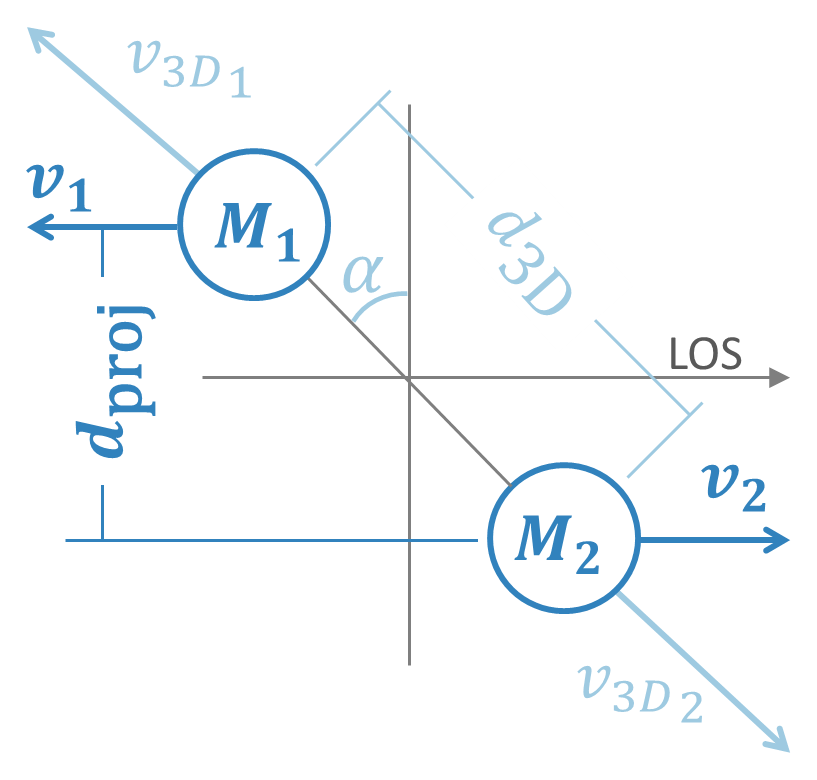
\includegraphics{Chapter3/MergerDiagram_revC.png}
\caption{The generic two-halo merger configuration assumed in this work.  Observable parameters are shown in dark blue, and include the mass of each halo ($M_i$), the  projected separation ($d_{\rm proj}$), and the line of sight (LOS) velocity components ($v_i$) as determined from the halo redshifts. 
The generally unknown parameters of the mergers are shown in light blue, and include the angle of the merger axis with respect to the plane of the sky ($\alpha$), and the three-dimensional separation ($d_{\rm 3D}$) and velocity components ($v_{\rm 3D_i}$).
Note that while just the outgoing scenario is shown in this figure, the method also considers the incoming scenario.
\label{fig_mergerdiagram}}
\end{figure}  

While the timing argument method is easy to use, its inherent assumptions result in non-negligible error for dissociative systems.
Most importantly the timing argument method assumes two point mass particles; this assumption begins to break down as the two subclusters overlap and results in divergent solutions as the subclusters near collision.
Since most dissociative mergers are observed with the two-subcluster halos overlapping and dark matter constraints depend on the merger dynamics near collision, application of the traditional timing argument to dissociative mergers is limited and should be done with caution.
\citet{Nusser:2008iw} addressed this weakness of the traditional timing argument by substituting truncated \citet*[][hereafter NFW]{Navarro:1996ce} halos and numerically solving the equations of motion.
Another weakness of the timing argument is that its main constraint requires the  assumption that the subcluster masses are constant since the beginning of the universe.  
While \citet{Angus:2007em} have noted this problem with the initial conditions of N-body simulations and proposed a solution based on estimating the mass accretion histories of the clusters \citep[e.g.][]{Wechsler:2002kh}, their correction is incompatible with the timing argument method as this would add a second differential term to the equations of motion.
Finally, the large covariance between the merger parameters plus the complexity of the equations of motion makes propagation of errors in the timing argument formalism untenable.
This has resulted in a lack of certainty with timing argument results, leaving most users to run a few scenarios in an effort to roughly bound the range of possible solutions \citep[e.g.][]{Boschin:2012he}.  

N-body simulations provide the most accurate description of merger dynamics, however they are computationally expensive which results in their application being limited.
Despite eleven currently confirmed dissociative mergers\footnote{(1) Bullet Cluster \citep{Clowe:2004eq}; 
(2) A520 \citep{Mahdavi:2007ed}; 
(3) MACS J0025.4-1222 \citep{Bradac:2008gw}; 
(4) A1240 \citep{Barrena:2009to}; 
(5) ZwCL 0008.8+5215 \citep{vanWeeren:2011ko}; 
(6) A2744 \citep{Merten:2011gu}; 
(7) A2163 \citep{Okabe:2011gv}; 
(8) A1758N \citep{Ragozzine:2011jj}; 
(9) Musket Ball Cluster \citep{Dawson:2012dl}; 
(10) ACT-CL J0102−4915 \citep{Menanteau:2012bf}; 
(11) MACS J0717.5+3745 \citep{Mroczkowski:2012vs}} only the Bullet Cluster has been modeled with N-body simulations, whereas most of these have been analyzed with the timing argument method.
Existing N-body simulation strategies to ascertain the dynamic properties of mergers are incapable of keeping up with the current faster than exponential rate of discovery.
Even for the case of the Bullet Cluster the N-body analyses have been limited as far as mapping out the merger dynamic phase space allowed by  the uncertainty of the observations, with at most 15 different scenarios being run \citep{Mastropietro:2008fs}.
\citet{Gomez:2012ex} have come the closest to addressing this issue in their investigation of potential dissociative mergers (A665 and AS1063) through the use of simplified scale-free numerical simulations of the mergers \citep[see][for details]{Gomez:2000kj}.  
However, they have still had to severely limit the phase space probed (fixing merger parameters such as the initial relative velocity and subcluster-subcluster mass ratio); thus admittedly this approach enables construction of plausible models, but not a thorough accounting of possible or likely models.

%%%% Task

With these weaknesses in mind I present a new method\footnote{This method is similar to the one used by \citet{Dawson:2012dl}, although with several improvements (see \S\ref{sec_musketball}).}  for analyzing the dynamics of observed dissociative mergers.
My primary objectives are to 1) obtain a solution valid near the collision state, 2) fully estimate the covariance matrix for the merger parameters, 3) be able to analyze a dissociative merger on the order of a day using a typical desktop computer, and 4) obtain approximately 10\% accuracy; all assuming that only the most general merger observables and their uncertainty are known: mass of each subcluster, redshift of each subcluster, and projected separation of the subclusters.

%%%% Object

In \S\ref{sec_method} I define a method for analyzing the dynamics of observed dissociative mergers.
In \S\ref{sec_sfcomp} I verify this method with existing results from a hydrodynamic N-body simulation.
In \S\ref{sec_bullet} I apply this method to the Bullet Cluster and in \S\ref{sec_musketball} I apply this method to the Musket Ball Cluster (DLSCL J0916.2+2951) and contrast its dynamics with those of the Bullet Cluster.
Finally in \S \ref{summary} I summarize my findings, discuss their implications for the constraints on dark matter and suggest other science that will benefit from the introduced method.
Throughout this paper I assume $\Omega_{\Lambda}=0.7$, $\Omega_m=0.3$, and $H=70$\,km\,s$^{-1}$\,Mpc$^{-1}$.




\section{Method}\label{sec_method}

In order to obtain a valid solution of the system dynamics near the collision state I use a model of two spherically symmetric NFW halos, rather than point masses.
I incorporate this model in a standard Monte Carlo implementation: draw randomly from the observables' probability density functions (PDF's) to generate a possible realization of the merger, use the model to calculate merger properties of interest, apply multiple priors, store these likelihood weighted results as a representative random draw of their PDF, and repeat.  
The final result is a multidimensional PDF for the dynamic parameters of the merger. 
This method agrees well with hydrodynamic simulations, \S\ref{sec_sfcomp}, and satisfies the speed and accuracy objectives outlined in the Introduction.

\subsection{Model}\label{sec_model}
The general basis of the model is a collisionless two body system with the mass of each body mutually conserved throughout the merger.
The model requires minimal input: the mass of each subcluster, the redshift of each subcluster, and the projected separation of the subclusters (along with associated uncertainties).
It assumes conservation of energy and zero angular momentum.
The model also assumes that the maximum relative velocity of the two bodies is the free-fall velocity of the system assuming their observed mass.
In the remainder of this subsection I will discuss in detail these general assumptions, their justification, and their implications. 

I model the system using two spherically symmetric NFW halos truncated at $r_{200}$\footnote{$r_{200}$ is defined as the radius of the spherical region within which the average density is 200 times the critical density at the respective redshift.}.  
By default the concentration of each halo is determined by the halo's mass via the mass-concentration scaling relation of \citet{Duffy:2008jy}.
This is not a requirement of the model though, and measured concentrations can be used, as in the case of \S\ref{sec_bc_obsprop}. 
The dynamic parameter results are relatively insensitive to the assumed concentration of the subclusters.  
Take for example the case of \S\ref{sec_sfcomp} with user specified concentrations of c$_1=1.94$ and c$_2=7.12$: if instead \citet{Duffy:2008jy} inferred concentrations c$_1=3.44$ and c$_2=2.75$ ($\sim200\%$ difference for both) are used, the difference in the estimated $v_{\rm 3D}(t_{\rm col})$ and $TSC$ are both less than 6\%.

The model assumes that the mass of each subcluster is constant and equal to the observed mass\footnote{For subcluster mass I refer to $M_{200}$, which is the mass of the individual subcluster enclosed within a radius of $r_{200}$.}.  
While this assumption is also used in the timing argument method, it is more reasonable for this method since the bulk of the results are calculated between the observed state and the collision state, typically lasting $\lesssim 1$\,Gyr.
This is about an order of magnitude shorter than the typical timescales of the timing argument method thus the new method is less susceptible to error due to neglecting growth of structure.

The model assumes that the energy of the two-halo system is conserved, and consists only of their mutual kinetic and potential energies.  
The kinetic energy of the system is $K(t) =  0.5 \mu v_{3D}(t)^2$, where $\mu$ is the reduced mass of the system and $v_{3D}(t)$ is the relative physical velocity of the two subclusters at time $t$.
The potential energy of the system is assumed to be purely gravitational and is derived in Appendix \ref{potentialsec}.
Since the model assumes zero impact parameter there is no rotational kinetic energy term.
\citet{Mastropietro:2008fs} find that a moderate impact parameter of $\sim0.1 r_{200}$ has less than a 1\% effect on the merger velocity, thus this assumption should have negligible effect for the case of dissociative mergers which must have had relatively small impact parameters in order to dissociate the bulk of their gas.

For the relative velocity of the two subclusters I apply a flat prior from zero to the free-fall velocity of the subclusters, assuming their observed mass.
This will result in an overestimate of the maximum possible relative velocity, due to the neglect of mass accretion.
It is conceivable that this prior could be tightened using the maximum relative velocities observed in cosmological N-body simulations as a function of subcluster masses and redshift. 
Another possibility for tightening the prior would be to analytically estimate the free-fall velocity accounting for mass accretion \citep[e.g.][]{Angus:2007em}.
An advantage of the Monte Carlo approach taken with this method is that additional priors can be applied as more knowledge becomes available without the need to rerun the analysis, so I opt for a conservative default approach.

The model ignores the effects of surrounding large scale structure and simply treats the two-body system.
As \citet{Nusser:2008iw} shows, a global overdense region (10 times denser than the background) engulfing the system only affects the dynamics substantially for extreme collision velocities ($\sim 4500$\,km\,s$^{-1}$).  While global overdensities may be disregarded it is not clear that the effects of nearby structures can be disregarded, e.g. as in the case three body systems.  Thus this method should be applied with caution to complex cluster mergers.

The model also ignores dynamical friction.
\citet{Farrar:2007fc} found that including dynamical friction accounted for an $\sim$10\% reduction in the inferred collision velocity of the Bullet Cluster in their analytic treatment.
This is potentially concerning since dynamical friction is inversely proportional to the relative velocity of the merger, thus it may become even more important for mergers slower than the Bullet Cluster.
However in \S \ref{sec_sfcomp} I compare the results of my method with those from a hydrodynamic N-body simulation and show that the net effect of all simplifications (including ignoring dynamical friction, tidal stripping of mass and gas mass lost during the collision) are negligible, suggesting that dynamic friction is less important than the analytic estimates of \citet{Farrar:2007fc} suggest.
 

\subsection{Monte Carlo Analysis}\label{sec_MCanalysis}

In this section I discuss the details of the Monte Carlo analysis workflow.
I chose to implement a Monte Carlo analysis because the high degree of correlation among the many merger dynamic parameters made traditional propagation of errors unfeasible.
A Monte Carlo analysis has the added advantage of easily enabling application of different combinations of priors ex post facto, see e.g. \S\ref{sec_addedprior}. 

The analysis begins by randomly drawing from the PDF's of the merger observables: mass of each subcluster ($M_{200_i}$), redshift of each subcluster ($z_i$), and projected separation of the subclusters ($d_{\rm proj}$).  The potential energy, $V$ (see Appendix \ref{potentialsec}), at the time of the collision is used to calculate the maximum relative velocity,
\begin{displaymath}
v_{\rm 3D_{max}} = \sqrt{-\frac{2}{\mu}V(r=0)}.
\end{displaymath}

The velocity of each subcluster relative to us is estimated from its redshift,
\begin{displaymath}
v_i = \left[\frac{(1+z_i)^2-1}{(1+z_i)^2+1}\right] c,
\end{displaymath}
where c is the speed of light.
The relative radial velocity of the subclusters is calculated from their redshifts,
\begin{displaymath}
v_{\rm rad}(t_{\rm obs}) = \frac{|v_2-v_1|}{1-\frac{v_1 v_2}{c^2}}.
\end{displaymath}

Since the angle of the merger axis with respect to the plane of the sky, $\alpha$, is unconstrained without prior knowledge of the three-dimensional relative velocity, I assume that all merger directions are equally probable.
However, projection effects result in $PDF(\alpha) = \cos(\alpha)$.
Due to symmetry it is only necessary to analyze the range $0\le\alpha\le 90$\,degrees.
I draw randomly from this PDF for each realization.
This enables the calculation of the three-dimensional relative velocity in the observed state, 
\begin{equation}
v_{\rm 3D}(t_{\rm obs}) = v_{\rm rad}(t_{\rm obs})/\sin(\alpha),
\label{eq_v3Dobs}
\end{equation}
as well as the observed three-dimensional separation of the subclusters, 
\begin{equation}
d_{\rm 3D}(t_{\rm obs}) = d_{\rm proj}/\cos(\alpha).
\label{eq_d3D}
\end{equation}

If $v_{\rm 3D}(t_{\rm obs}) > v_{\rm 3D_{max}}$, then this realization of the merger is discarded; otherwise the relative collision velocity is calculated,
\begin{equation}
v_{\rm 3D}(t_{\rm col}) = \sqrt{v_{\rm 3D}(t_{\rm obs})^2+\frac{2}{\mu}\left[V(t_{\rm obs})-V(t_{\rm col})\right]}.
\label{eq_v3Dcol}
\end{equation}
Similarly if $v_{\rm 3D}(t_{\rm col}) >v_{\rm 3D_{max}}$, then this realization is discarded.

The change in time, $\Delta t$, between two separations is given by
\begin{equation}
\Delta t = \int_{r_1}^{r_2} \frac{dr}{\sqrt{\frac{2}{\mu}(E-V(r))}}.
\label{eq_deltat}
\end{equation}
I define the time-since-collision ($TSC$) as the time it takes the subclusters to traverse from zero separation to their physical separation in the observed state, $d_{\rm 3D}$. 
Because there is a potential degeneracy in whether the subclusters are ``outgoing'' (approaching the apoapsis after collision)  or ``incoming'' (on a return trajectory after colliding and reaching the apoapsis); I solve for both of these cases, $TSC_0$ and $TSC_1$ respectively.
In determining $TSC_1$ it is useful to define the period, $T$, of the system.  I define $T$ to be the time between collisions,
\begin{displaymath}
T  = 2 \int_{0}^{d_{\rm max}} \frac{dr}{\sqrt{\frac{2}{\mu}(E-V(r))}},
\end{displaymath}
where $d_{\rm max}$ is the distance from zero separation to the apoapsis, when $E=V$.
Thus,
\begin{displaymath}
TSC_1 = T - TSC_0.
\end{displaymath}
During the Monte Carlo analysis any realizations with $TSC_0$ greater than the age of the Universe at the cluster redshift are discarded.
A similar flat prior is applied when calculating the statistics of $TSC_1$.
To this regard some insight into the likelihood of the system being in an ``outgoing'' or ``incoming'' state can be gained by calculating the fraction of realizations with $TSC_1$ less than the age of the Universe at the cluster redshift.
Conceivably these temporal priors could be strengthened, requiring that the time to first collision ($T$) plus the respective $TSC$ be less than the age of the Universe at the cluster redshift, in a fashion similar to the timing argument.
However, as with the timing argument model, the model of \S\ref{sec_model} becomes less valid over time-scales approaching the age of the Universe.
Thus I use the more conservative prior by default.

Since the majority of the merger time is spent at large separations, due to lower relative velocities, observations of the system are more likely near apoapsis than near the collision.  Thus the probability of each realization is convolved with the prior 
\begin{equation}
{\rm PDF}(TSC_0) = 2 \frac{TSC_0}{T}.
\label{eq_timeprior}
\end{equation}
There are likely selection effects which complicate this PDF, since it can be imagined that the X-ray luminosity is greatest near the time of the collision \citep[see e.g.][]{Randall:2002kk}.
However this information is rarely if ever known, thus it is not included by default.  In \S\ref{sec_addedprior} I show how additional temporal priors, based on similar effects, may be effectively applied to the results of the analysis ex post facto.

The end result of this method is a 13 dimensional posterior PDF of an array of cluster merger parameters, see for example Appendix \ref{sec_bcresults}.
Finally to compact the results I use the biweight-statistic (generally more robust and less sensitive to abnormally tailed distributions than the median or mean) and bias-corrected percent confidence limits \citep{Beers:1990kg} applied to the marginalized parameter distributions of the valid realizations, see for example Table \ref{bulletresultparam}.


\subsection{Comparison with Hydrodynamic Simulations} \label{sec_sfcomp}

For the purposes of checking the physical assumptions of the model I reanalyze the \citet{Springel:2007bg} model of the Bullet Cluster, comparing my dynamic parameter estimates with their hydrodynamic N-body simulation based estimates.
For this analysis I run just their single case through the model (i.e.\,I do not perform a Monte Carlo analysis).
They represent the ``main'' and ``bullet'' subclusters as NFW halos with  M$_{200_1} = 1.5\times 10^{15} $\,M$_\sun$, c$_1=1.94$, M$_{200_2} = 1.5\times 10^{14}$\,M$_\sun$, and c$_2=7.12$, respectively.
They note that the gas properties of their simulation most closely match the observed Bullet Cluster gas properties for the time step corresponding to a subcluster separation of $d_{3D}=625$\,kpc and  relative velocity of $v_{\rm 3D}(t_{\rm obs})=2630$\,km\,s$^{-1}$.
I define this as the ``observed'' state (dashed line in Figure \ref{fig_SFcomparison}) and use the model discussed in \S \ref{sec_model} to extrapolate values of the relative subcluster velocities ($v_{\rm 3D}$) and time-since-observed state (TSO) before and after the observed state (left and right of the dashed line in Figure \ref{fig_SFcomparison}, respectively).
The \citet{Springel:2007bg} simulation results (black circles) for these parameters are read directly from their Figure 4.

I compare the model results (blue boxes) with the \citet{Springel:2007bg} simulation results, and assume their results as truth when calculating the percent error, see Figure \ref{fig_SFcomparison}.
There is better than 4\% agreement between $v_{\rm 3D}$ and 14\% agreement between the TSO.
While the model results are biased, the bias appears stable and is roughly an order of magnitude smaller than the typical random error in the parameter estimates (see for example Table \ref{bulletresultparam}).
Given the stability of the bias it is conceivable that it could be corrected in the model results.
However, to have any confidence in this bias correction the model results should be compared with a range of merger scenarios, which is beyond the scope of this current work.
Note that the better agreement between the velocity estimates than between the TSO estimates is to be expected since the velocity calculation (essentially Equation \ref{eq_v3Dcol}) comes from simply comparing the observed and another state of the merger whereas the TSO calculation (Equation \ref{eq_deltat}) requires integration between these two states.
The results of this comparative study essentially validate many of the simplifying assumptions of the model (conservation of energy, and ignoring the affects of dynamical friction, tidal stripping of dark matter and gas during the collision).

\begin{figure}
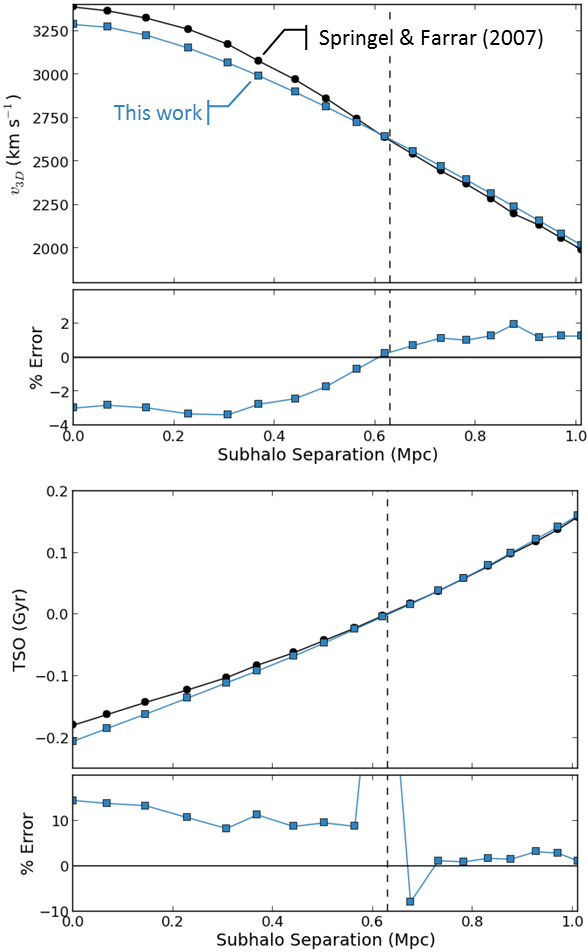
\includegraphics{Chapter3/SFcomparison.png}
\caption{
Comparison of the model results (blue boxes) with the hydrodynamic simulation results of \citet[black circles;][]{Springel:2007bg} for the Bullet Cluster.  
The top figure is a comparison of the velocity of the ``bullet'' relative to the ``main'' subcluster, with the subhalo separation (i.e. the three-dimensional separation of the ``main'' and ``bullet'' subclusters) as the independent variable.  
The bottom figure is a comparison of the time-since-observed state (TSO), where the ``observed'' state (dashed line) is defined by \citet{Springel:2007bg} as the time step in their simulation when the gas properties most closely match the observed Bullet Cluster gas properties.
Times prior(post) to the observed state have negative(positive) values.  
The percent error in each case is calculated assuming the \citet{Springel:2007bg} results as truth.  
While the model results are biased, the bias appears stable and is roughly an order of magnitude smaller than the typical random error in the parameter estimates (see for example Table \ref{bulletresultparam}).  
Note that the TSO percent error calculation understandably diverges near the arbitrary choice of time equal zero. 
The \citet{Springel:2007bg} results are read directly from their Figure 4.
\label{fig_SFcomparison}}
\end{figure}

As an aside it should be noted that for this comparison I use the \citet{Springel:2007bg} NFW halo parameters that represent the state of the halos prior to collision.
Ideally I should use the NFW parameters representative of the state of the halos at $t_{\rm obs}$, however these properties were not reported in their paper.
From Figure 5 of \citet{Springel:2007bg} some insight into the time variability of the halo parameters can be gained.
Since the depth each halo's gravitational potential at $\sim r_{200}$ does not change appreciably throughout the merger, it can be inferred that M$_{200}$ of each halo does not change. 
However, the gravitational potential near the center of each halo deepens by $\sim 25\%$ during and after the collision.
This can be interpreted as the concentration of each halo increasing.
Thus for the comparison of my model with the \citet{Springel:2007bg} hydrodynamic simulation to be more appropriate I should have used halos with larger concentrations.
Doing so actually brings my model results more in-line with the simulation results.
If for example I increase the concentration of the ``bullet'' halo from 1.94 to 3 and the concentration of the ``main'' halo from 7.12 to 8, then the percent error for the relative velocity of the halos reduces to $\lesssim 1\%$ and the percent error for the TSO reduces to $\sim 10\%$. 
Thus the comparative results of Figure \ref{fig_SFcomparison} should be considered conservative with respect to the variability of the halo properties throughout the merger.

%\begin{deluxetable}{lcc}
%\tablewidth{0pt}
%%\tabletypesize{\scriptsize}
%\tablecaption{Comparison of the model results with hydrodynamic simulation results\label{modeltest}}
%
%\tablehead{
%\colhead{Work}     & \colhead{$v_{\rm 3D}(t_{\rm col})$}  & \colhead{TSC$_0$}  \\
%\colhead{}     &  \colhead{km\,s$^{-1}$}  & \colhead{Gyr}
%}
%\startdata
%\citet{Springel:2007bg} & 3400 &  0.18 \\
%This work  & 3380 & 0.198 \\
%\hline
%\% Error & 0.70 & 10\\ 
%\enddata
%\end{deluxetable}


\section{Bullet Cluster Dynamics}\label{sec_bullet}

The Bullet Cluster is the prime candidate for first application of the method as it is one of the best studied dissociative mergers.
It has a wealth of observational data necessary for input to the model, as discussed in \S\ref{sec_bc_obsprop}, plus supplementary data which enables additional posterior priors, as discussed in \S\ref{sec_addedprior}.
%Additionally it has been studied using basic CDM N-body simulations, hydrodynamic simulations and SIDM simulations.

\subsection{Bullet Cluster Observed System Properties}\label{sec_bc_obsprop}

I summarize the observed Bullet Cluster parameters used as input to my analysis in Table \ref{bulletinputparam}.  
The full PDF's of these input parameters have not been published so I simply assume Gaussian distributions.
I refer to the main subcluster as halo 1 and the ``bullet'' subcluster as halo 2.  
For the mass and concentration of each subcluster I use the most recently reported estimates from \citet{Springel:2007bg}, based upon strong and weak lensing estimates \citep{Bradac:2006be}.
However, they do not present errors for these quantities so for the mass I estimate the  1--$\sigma$ errors to be 10\% of the mass, since this is approximately the magnitude of the error reported by \citet{Bradac:2006be} for M($<250$\,kpc).
There is no published estimate for the uncertainty of the concentrations of the NFW model fits, $c_i$, so I simply assume the concentrations to be known quantities (as noted in \S\ref{sec_model} the results are relatively insensitive to the assumed concentrations). 
The redshifts of the main and ``bullet'' subclusters are estimated from 71 and 7 spectroscopic members, respectively \citep{Barrena:2002dj}.
The projected separation of the mass peaks is determined from strong and weak lensing measurements \citep{Bradac:2006be}, and is essentially the same as the separation of the subclusters' galaxy centroids.
For each Monte Carlo realization individual values are drawn randomly from each of these assumed Gaussian distributions.

\begin{deluxetable}{lcccc}
\tablewidth{0pt}
%\tabletypesize{\scriptsize}
\tablecaption{Bullet Cluster parameter input\label{bulletinputparam}}

\tablehead{
\colhead{Parameter}     & \colhead{Units}  & \colhead{$\mu$}  & \colhead{$\sigma$}	&	\colhead{Ref.}
}
\startdata
M$_{200_1}$	&	$10^{14}$\,M$_\sun$	&	15	&	1.5\tablenotemark{a}	&	1	\\
c$_1$	&		&	7.2	&	\nodata\tablenotemark{b}	&	1	\\
M$_{200_2}$	&	$10^{14}$\,M$_\sun$	&	1.5	&	0.15\tablenotemark{a}	&	1	\\
c$_2$	&		&	2.0	&	\nodata\tablenotemark{b}	&	1	\\
z$_1$	&		&	0.29560	&	0.00023	&	2	\\
z$_2$	&		&	0.29826	&	0.00014	&	2	\\
$d_{\rm proj}$		&	kpc	&	720	&	25	&	3	\\
\enddata
\tablecomments{A Gaussian distribution with mean, $\mu$, and standard deviation, $\sigma$, is assumed for all parameters with quoted respective values.  The mass, M$_{200}$, and concentration, c, are the defining properties of assumed spherically symmetric NFW halos.}
%\tablenotetext{a}{Estimated to be 10\%, based one the error magnitude of M($<250$\,kpc) reported in Brada{\v c} et al. (2006).}
\tablenotetext{a}{Estimated to be 10\%, based one the error magnitude of M($<250$\,kpc) reported in \citet{Bradac:2006be}.}
\tablenotetext{b}{No errors were presented in the reference.  A single concentration value was used for all Monte Carlo realizations.}
\tablerefs{
(1) Springel \& Farrar 2007; (2) Barrena et al. 2002; (3) Brada{\v c} et al. 2006.}
\end{deluxetable}

\subsection{Bullet Cluster System Dynamics Results} \label{bulletdynamics}

I first analyze the Bullet Cluster with the Monte Carlo analysis method and default priors discussed in \S\ref{sec_method}, highlighting the complexity of merger dynamics and the inappropriateness of analyzing a small sample of select merger scenarios.
In \S\ref{sec_addedprior} I incorporate  additional constraints provided by the observed strong X-ray shock front plus boosted temperature and luminosity.
I discuss this prior information and apply it ex post facto to the default prior results of \S\ref{sec_defaultprior}.

I perform the analysis with 2,000,000 Monte Carlo realizations.  
Parameter estimates converge to better than a fraction of a percent with only 20,000 realizations ($\sim6$\,CPU\,hours).
I run a factor of a hundred more since it was computationally inexpensive and it provides a data sample to which I can apply any number of conceivable posterior PDF's and still maintain sub-percent statistical accuracy.

\begin{figure}
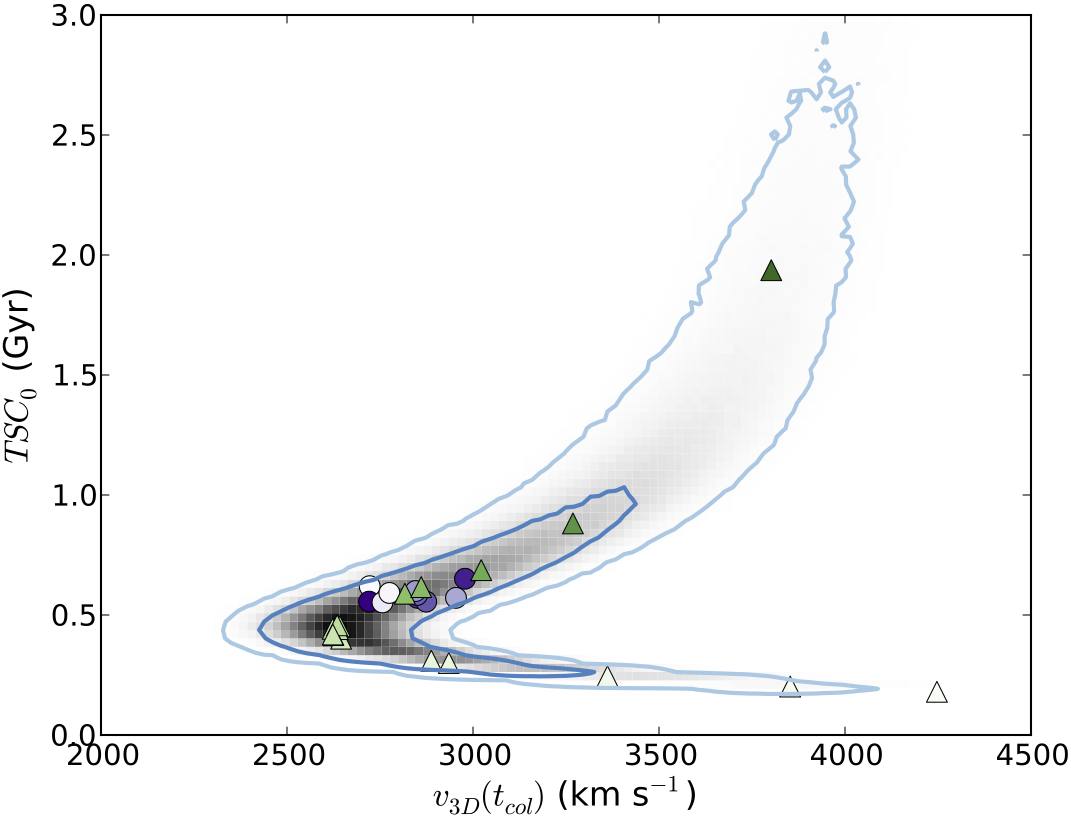
\includegraphics[scale=1.15]{Chapter3/peakvalues_revB.png}
\caption{
The posterior of the Bullet Cluster's time-since-collision $TSC_0$ and $v_{\rm 3D}(t_{\rm col})$ parameters is shown in grayscale with dark and light blue contours representing 68\% and 95\% confidence, respectively.
The green-scale triangles are from a subsample of the Monte Carlo population, which jointly satisfies the requirement of being drawn from $\pm 0.01 \sigma$ of the mean of each of the input parameters, i.e. the ``most likely'' values for the input parameters. 
Despite representing the most probable input parameter values there is considerable spread in the inferred output parameters, with the subsample clearly tracing the ridge of the distribution. 
The saturation of the triangles increases with increasing $\alpha$, from 10--86\,degrees.
The purple-scale circles are from a subsample near the bi-weight location of $\alpha=50\pm0.0002$\,degrees, with the saturation of the circles increasing with increasing M$_{200_1}$.
While the length of the distribution is predominantly caused by uncertainty in $\alpha$ the width is predominantly caused by uncertainty in the input parameters.
Despite the Bullet Cluster being one of the best measured dissociative mergers there is still considerable and complex uncertainty in its merger parameters, predominantly due to uncertainty in $\alpha$. 
\label{fig_bcTSC}}
\end{figure}


\subsubsection{Default Priors}\label{sec_defaultprior}

The main results of this analysis are that: 1) there is a great degree of covariance between the geometry, velocity, and time parameters of the merger, and 2) models of the system which disregard the uncertainty of $\alpha$ will catastrophically fail to capture the true uncertainty in the dynamic parameters.

The two-dimensional PDF of Figure \ref{fig_bcTSC} exemplifies the complexity of the covariance between the various merger parameters\footnote{Similar degrees of complex covariance exist for the other geometry, velocity and time parameters, see e.g.\,the results array in Appendix \ref{sec_bcresults}.}.
The shape of the PDF is most easily understood in terms of the parameters' dependence on $\alpha$.
This dependence is illustrated by the green-scale triangles that represent a subsample of the Monte Carlo population,  which jointly satisfies the requirement of being drawn from $\pm 0.13 \sigma$ of the mean of each of the input parameters, i.e. the ``most likely'' values for the input parameters.
The saturation of the triangles increases with increasing $\alpha$, from 10--86\,degrees, clearly showing a monotonically increasing relationship with $TSC_0$ (see also Figure \ref{fig_bc_geovt}).
For small $\alpha$ (light green triangles), Equation \ref{eq_v3Dobs} states that $v_{\rm 3D}(t_{\rm obs})$ must be large thus $v_{\rm 3D}(t_{\rm col})$ must also be large, and since Equation \ref{eq_d3D} states that $d_{\rm 3D}(t_{\rm obs})$ approaches the minimum possible observed separation, $d_{\rm proj}$, the $TSC_0$ must approach a minimum.
Conversely for large $\alpha$ (dark green triangles), $d_{\rm 3D}(t_{\rm obs})$ becomes large increasing the time required to reach the observed state, and despite $v_{\rm 3D}(t_{\rm obs})$ approaching the minimum $v_{\rm rad}(t_{\rm obs})$ the collision velocity must increase for the subclusters to have been able to reach the larger $d_{\rm 3D}(t_{\rm obs})$.   

The bulk of the uncertainty in the geometry, velocity and time parameters is due to the uncertainty of $\alpha$.
This is exemplified by the fact that the green-scale triangles in Figure \ref{fig_bcTSC} closely trace the extent of the ridge line of the two-dimensional distribution (i.e. span the bulk of the uncertainty).
Conversely the ``width'' of the distribution is predominantly due to uncertainty in the input parameters.
This is exemplified by the purple circles of Figure \ref{fig_bcTSC}, which are for a near constant $\alpha$ yet randomly sample the M$_{200_1}$ distribution. 
The saturation of the circles increase with increasing mass.

The inability to directly measure $\alpha$, coupled with its strong degree of correlation with the other dynamic parameters, makes it the dominant source of uncertainty. 
While it was originally believed that the three-dimensional merger velocity as inferred from the X-ray shock feature could be coupled with the redshift determined radial velocity to measure $\alpha$, \citet{Springel:2007bg} showed that the X-ray shock inferred velocity significantly overestimates the true three-dimensional merger velocity.
So at best this information can weakly constrain $\alpha$, and in the case of the Bullet Cluster the X-ray shock inferred velocity is significantly greater than the free-fall velocity, $v_{\rm 3D_{max}}$, thus it provides no additional constraining power.
In \S\ref{sec_suggestions} I discuss how the results of this method can be used in conjunction with N-body simulations to limit the computational impact of accounting for the uncertainty in $\alpha$.



\begin{deluxetable*}{lc|ccc|ccc}
\tablewidth{0pt}
%\tabletypesize{\scriptsize}
\tablecaption{Bullet Cluster parameter estimates\label{bulletresultparam}}
\tablehead{																							
Parameter     & Units  & 
\multicolumn{3}{|c|}{Default Priors}  & \multicolumn{3}{|c}{Default + Added Temporal Priors}
\\
     &   & 
\colhead{Location\tablenotemark{a}}  & \colhead{68\% LCL--UCL\tablenotemark{b}} & \colhead{95\% LCL--UCL\tablenotemark{b}}	& 
\colhead{Location\tablenotemark{a}}  & \colhead{68\% LCL--UCL\tablenotemark{b}} & \colhead{95\% LCL--UCL\tablenotemark{b}}	
}					
\startdata																							
M$_{200_1}$	&	$10^{14}$\,M$_\sun$	&	
15.0	&	13.5	--	16.6	&	12.1	--	18.1	&	
15.2	&	13.6	--	16.6	&	12.2	--	18.1	\\
M$_{200_2}$	&	$10^{14}$\,M$_\sun$	&	
1.5	&	1.4	--	1.6	&	1.2	--	1.8	&	
1.5	&	1.4	--	1.7	&	1.2	--	1.8	\\
$z_1$	&		&	
0.2956	&	0.2954	--0.2958	&	0.2951 --0.2961	&	
0.2956	&	0.2954	--0.2958	&	0.2951 --0.2961	\\
$z_2$	&		&	
0.2983	&	0.2981	--	0.2984	&	0.2980	--	0.2985	&	
0.2983	&	0.2981	--	0.2984	&	0.2980	--	0.2985	\\
$d_{\rm proj}$	&	Mpc	&	
0.72	&	0.69	--	0.76	&	0.65	--	0.80	&	
0.72	&	0.68	--	0.75	&	0.64	--	0.79	\\
$\alpha$	&	degree	&	
50	&	27	--	73	&	15	--	84	&	
24	&	16	--	38	&	11	--	53	\\
$d_{\rm 3D}$	&	Mpc	&	
1.1	&	0.8	--	2.6	&	0.7	--	7.1	&	
0.8	&	0.7	--	0.9	&	0.7	--	1.2	\\
$d_{\rm max}$	&	Mpc	&	
1.3	&	1.1	--	2.5	&	1.0	--	6.4	&	
1.2	&	1.0	--	1.7	&	1.0	--	3.1	\\
$v_{\rm 3D}(t_{\rm obs})$	&	km\,s$^{-1}$	&	
820	&	640	--	1500	&	550	--	2500	&	
1600	&	1100	--	2500	&	790	--	3200	\\
$v_{\rm 3D}(t_{\rm col})$	&	km\,s$^{-1}$	&	
3000	&	2700	--	3800	&	2500	--	4200	&	
2800	&	2600	--	3300	&	2500	--	3800	\\
$TSC_0$	&	Gyr	&	
0.6	&	0.3	--	1.1	&	0.2	--	3.9	&	
0.4	&	0.3	--	0.5	&	0.2	--	0.6	\\
$TSC_1$\tablenotemark{c} &	Gyr	&	
1.2	&	1.0	--	2.4	&	0.9	--	8.2	&	
1.3	&	1.0	--	2.0	&	0.9	--	4.6	\\
$T$	&	Gyr	&	
1.8	&	1.5	--	3.2	&	1.4	--	8.1	&	
1.6	&	1.4	--	2.3	&	1.3	--	4.8	\\
\enddata																							
\tablenotetext{a}{Biweight-statistic location \citep[see e.g.][]{Beers:1990kg}.}																							
\tablenotetext{b}{Bias-corrected lower and upper confidence limits, LCL and UCL respectively \citep[see e.g.][]{Beers:1990kg}.}
\tablenotetext{c}{For the case of the Default + Added Temporal Prior, none of the realizations have a valid $TSC_1$, meaning that the Bullet Cluster is being observed in the ``outgoing'' state, as discussed in \S\ref{sec_addedprior}.}
\end{deluxetable*}	

\subsubsection{Added Temporal Prior}\label{sec_addedprior}

One of the advantages of this Monte Carlo method is that additional constraints are easily incorporated ex post facto.
An example of such constraints in the case of the Bullet Cluster is the observed X-ray shock front and factor of 2.4 greater X-ray estimated mass to lensing estimated mass \citep{Markevitch:2006wv}, due to merger related X-ray temperature and luminosity boost.  
Hydrodynamic simulations of merging clusters \citep[e.g.][]{Ricker:2001ju,Randall:2002kk} suggest that such transient effects last of order the X-ray sound crossing time.
Since simulations show negligible difference between the time scales of the two I chose to construct a prior based on the observed temperature boost.
\citet{Randall:2002kk} find that the full-width-half-max (FWHM) duration of the temperature boost is $\sim 0.4 t_{\rm sc}$ with the entire boost duration being $\sim 1.4 t_{\rm sc}$, where $t_{\rm sc}$ is the sound crossing time of the more massive of the two subclusters.
The peak of this boost roughly coincides with the time of the \emph{collision}, as defined in \S\ref{sec_intro}.
Given the M$_{200_1}=15 \times 10^{14}$\,M$_\sun$ and temperature T$_{\rm X}=14$\,keV of the ``main'' subcluster \citep{Markevitch:2006wv}, the $t_{\rm sc}=1$\,Gyr.
I construct a sigmoid function for the $TSC$ prior PDF based on the observed temperature boost, 
\begin{displaymath}
{\rm PDF}(TSC) = \frac{1}{2}\left[1-\tanh\left(\frac{TSC-0.5 a}{0.25 b} \right)\right],
\end{displaymath}
where $a$ is the FWHM of the duration of the temperature boost and $b$ is the entire boost duration.
I chose a sigmoid function over a simple step function since the temperature boost predicted by \citet{Randall:2002kk} does not end abruptly.
This prior is coupled with the previously discussed $TSC$ prior (Equation \ref{eq_timeprior}).

\begin{figure}
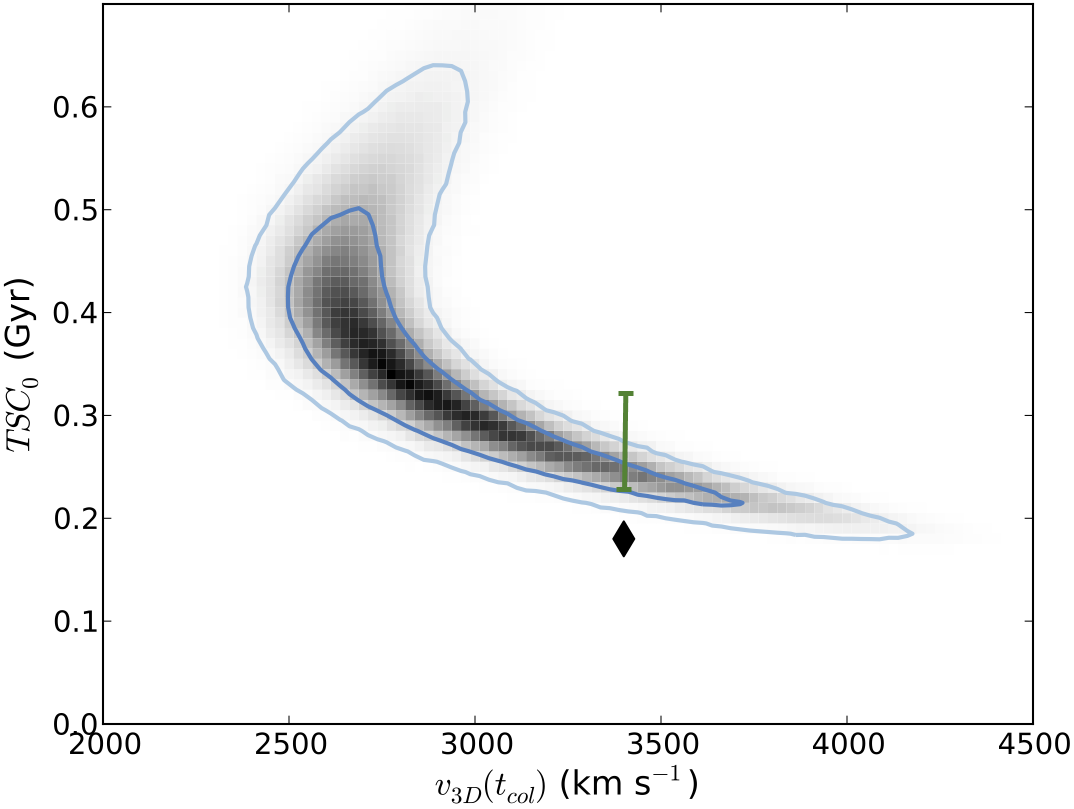
\includegraphics[scale=1.15]{bullet_VvsTSC_addedprior.png}
\caption{
The posterior of the Bullet Cluster's $TSC_0$ and $v_{\rm 3D}(t_{\rm col})$ parameters after application of an additional temporal prior based on X-ray observations of the Bullet Cluster (grayscale).  
Dark and light blue contours representing 68\% and 95\% confidence, respectively.
The added temporal prior significantly improves the constraint on the merger parameters (compare with Figure \ref{fig_bcTSC}).
The black diamond represents the Springel \& Farrar (2007) hydrodynamic simulation result for their defined ``observed state'', whose X-ray properties best match the observed X-ray properties; $d_{\rm 3D}$=625\,kpc for this state.
The green bar shows their result for $d_{\rm 3D}$ between 700 to 900\,kpc, which is more in line with the observed $d_{\rm proj} = 720\pm 25$\,kpc (assuming $0<\alpha<35$\,degrees).
\label{fig_bcTSC_added}}
\end{figure}

Application of this prior significantly improves the uncertainty in $TSC_0$ (180\% to 67\%)  and $v_{\rm 3D}(t_{\rm col})$ (28\% to 19\%), compare Figure \ref{fig_bcTSC} with Figure \ref{fig_bcTSC_added}.
It essentially removes the possibility of a $TSC > 0.6$\,Gyr.
As expected from the $\alpha$ dependence shown by the green triangles in Figure \ref{fig_bcTSC} this prior also reduces the likelihood of $\alpha \gtrsim 50$\,degrees, which in turn affects both the location and uncertainty of $d_{\rm3D}$ and $v_{\rm 3D}(t_{\rm obs})$, see Table \ref{bulletresultparam}. 
The remaining parameter estimates are predominantly unaffected by the prior, with only a few having their confidence limits affected as the result of their high end low probability tails being down weighted.
Additionally there is now essentially zero probability that the bullet subcluster has reached the apoapsis and is on a return trajectory, since the 95\% lower confidence limit of $TSC_1$ is 0.9\,Gyr (see Table \ref{bulletresultparam}) and the prior essentially removes the possibility of a $TSC > 0.6$\,Gyr.
I present the full results array, which includes the default analysis prior combined with this temperature boost prior, in Appendix \ref{sec_bcresults} and the compact parameter estimates in Table \ref{bulletresultparam}.

According to this analysis the \citet{Springel:2007bg} results stated in \S\ref{sec_sfcomp} seem unlikely (see the black diamond of Figure \ref{fig_bcTSC_added}), however this is simply due to their definition of the ``observed state''.
They define the observed state to be when their simulated X-ray properties most closely match the observed X-ray properties, yet the separation of the halos in this state is only $d_{\rm 3D}=625$\,kpc; this is less than the observed $d_{\rm proj} = 720\pm 25$\,kpc \citep{Bradac:2006be}.
If we instead consider their estimate of $TSC_0$ for $d_{\rm 3D}$ between 700 to 900\,kpc (corresponding to  $d_{\rm proj} = 700$ and $0<\alpha<35$\,degrees), then $0.24<TSC_0<0.33$\,Gyr (see green bar of Figure \ref{fig_bcTSC_added}).
This brings their result in line with the results of this method, as expected by the agreement presented in \S\ref{sec_sfcomp}.
Note that the general conclusion of \citet{Springel:2007bg}, that the  shock speed greatly overestimates the actual relative speed of the subclusters, remains valid regardless of which ``observed state'' is used.

\section{Musket Ball Cluster Dynamics}\label{sec_musketball}

I also apply the method to the Musket Ball Cluster, with the objective of updating an existing analysis and comparing this system with the Bullet Cluster.  
A preliminary analysis of the system dynamics using a similar method \citep{Dawson:2012dl} suggested that the Musket Ball Cluster merger is $\sim$3--5 times further progressed than other confirmed dissociative mergers.
However, that analysis treated the two merging subclusters as uniform density spheres   and also failed to account for the temporal phase-space PDF (Equation \ref{eq_timeprior}).
Additionally the claim that the Musket Ball Cluster is both slower and further progressed than the Bullet Cluster was based on comparing the Musket Ball's $TSC_0$--$v_{\rm 3D}(t_{\rm col})$ PDF with that of the single point \citet{Springel:2007bg} estimate.
As noted in \S\ref{sec_defaultprior} there is a large area of parameter space that the \citet{Springel:2007bg} result fails to represent.

Similar to my analysis of the Bullet Cluster I perform the analysis with 2,000,000 Monte Carlo realizations.
Parameter estimates converge to better than a fraction of a percent with only 20,000 realizations.

\subsection{Musket Ball Observed System Properties}

I show the observed Musket Ball Cluster parameter PDF's in Figures \ref{musket_massinput}--\ref{musket_projinput}, each the result of analyses presented by \citet{Dawson:2012dl}.  
I refer to their ``south'' subcluster as halo 1 and ``north'' subcluster as halo 2. 
The mass PDF's, Figure \ref{musket_massinput}, are the result of an MCMC analysis where NFW halos were simultaneously fit to the weak lensing signal.
The relative velocity distributions, Figure \ref{musket_vinput}, are the result of a bootstrap error analysis \citep{Beers:1990kg} of the 38 and 35 spectroscopic members of the north and south subclusters, respectively.
These redshifts as well as the full Musket Ball Cluster spectroscopic catalog are presented in Table \ref{table_MBCzcat} of Appendix \ref{sec_MBCzcat}.
The projected subcluster separation distribution, Figure \ref{musket_projinput}, is the result of a bootstrap error analysis of the recursively estimated subclusters' galaxy number density centroids \citep[see e.g.][for a description of this method]{Randall:2008hs}.
For each Monte Carlo realization individual values are drawn randomly from each of these distributions. 

\begin{figure}
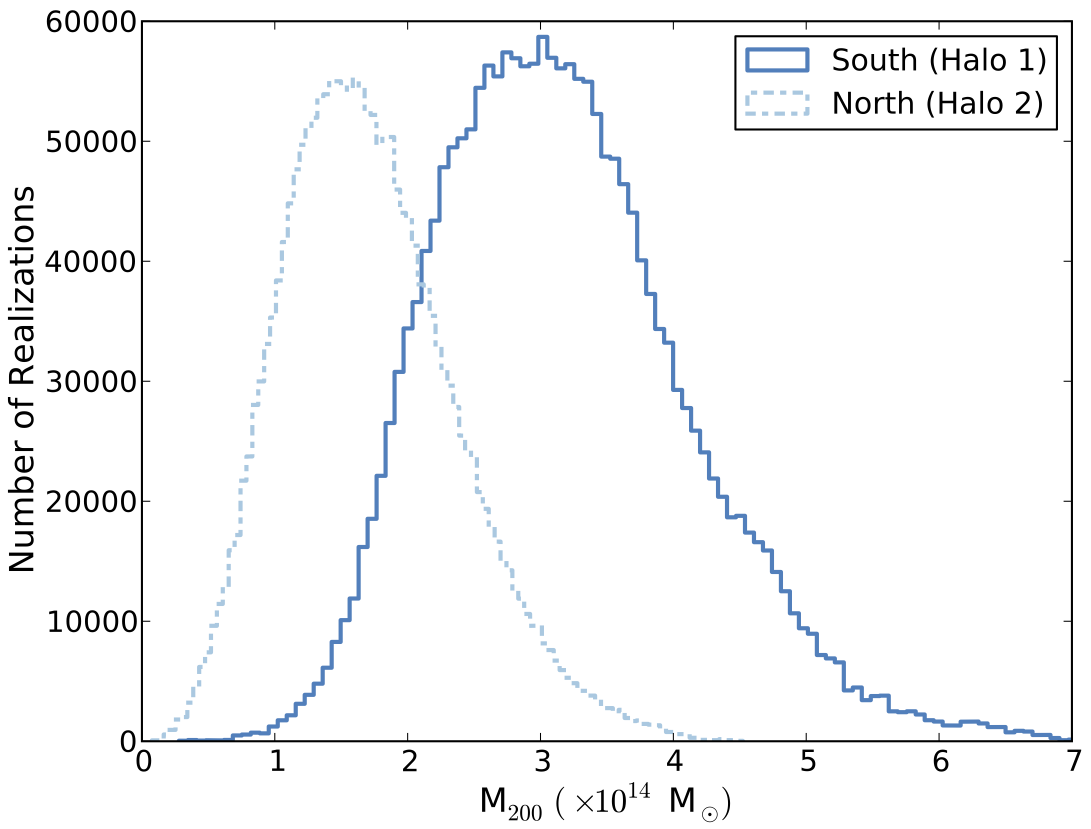
\includegraphics{Chapter3/MusketBall_mass_input_revB.png}
\caption{Weak lensing mass PDF's of the Musket Ball subclusters \citep{Dawson:2012dl}. 
\label{musket_massinput}}
\end{figure}

\begin{figure}
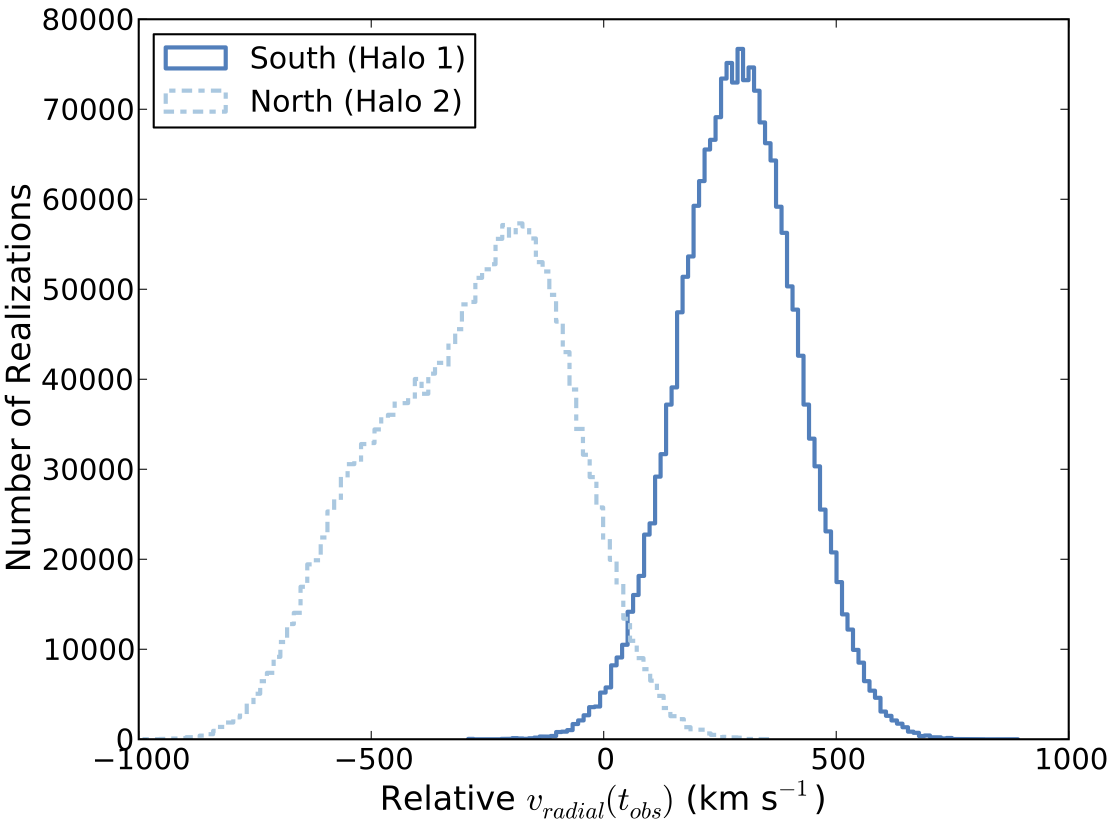
\includegraphics{Chapter3/MusketBall_velocity_input_revB.png}
\caption{Relative radial subcluster velocity PDF's inferred from spectroscopic redshifts the Musket Ball Cluster galaxies  \citep{Dawson:2012dl}. 
\label{musket_vinput}}
\end{figure}

\begin{figure}
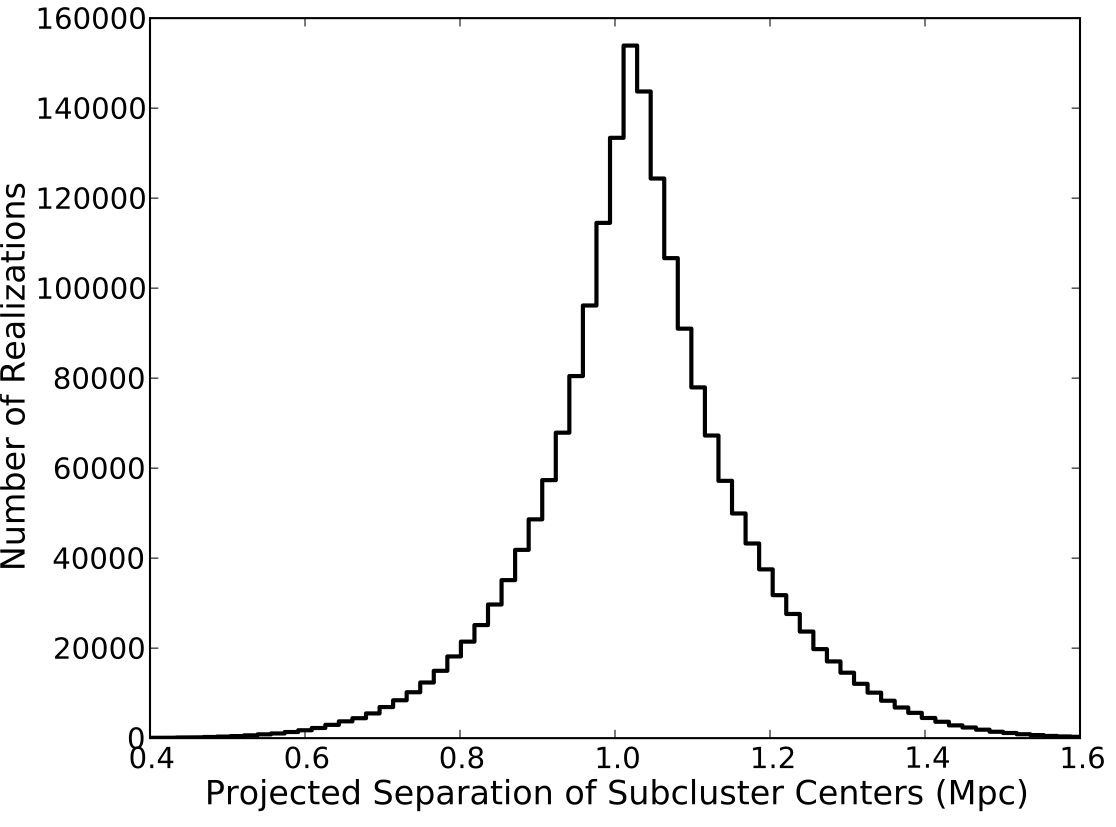
\includegraphics{Chapter3/MusketBall_projsep_input_revB.png}
\caption{Projected separation PDF of the Musket Ball subcluster galaxy density centroids \citep{Dawson:2012dl}. 
\label{musket_projinput}}
\end{figure}

\subsection{Musket Ball System Dynamics Results}

This more complete analysis confirms that the Musket Ball Cluster merger is both significantly slower and further progressed compared to the Bullet Cluster, see Figure \ref{fig_mbc_TSC}.
To estimate a lower limit on how much further progressed I perform an additional Monte Carlo analysis  for $TSC_{\rm 0_{Musket}}-TSC_{\rm 0_{Bullet}}$ assuming the marginalized $TSC_0$ distributions (see Appendices \ref{sec_bcresults} and \ref{sec_mbcresults}).
This is a lower limit since the Musket Ball observations, unlike the Bullet Cluster observations, cannot rule out the case that its subclusters have reached the apoapsis and are on a return trajectory (61\% of the realizations have $TSC_1$ less than the age of the Universe at $z=0.53$).
I find that  the Musket Ball is at least $0.8^{+1.2}_{-0.4}$\,Gyr ($3.4^{+3.8}_{-1.4}$ times) further progressed than the Bullet Cluster, see Figure \ref{fig_TSC0comparison}.
This is in line with the more approximate 3--5 times estimate of \citet{Dawson:2012dl}.
The Musket Ball's relatively large $TSC_0$ means that it has potential for providing tighter constraints on $\sigma_{\rm DM}$, since the expected offset between the galaxies and dark matter will initially increase with increasing $TSC_0$.
However as noted in \S\ref{sec_intro}, given enough time the expected offset will decrease due the gravitational attraction between the galaxies and dark matter.
Also important in determining which cluster can provide the tightest $\sigma_{\rm DM}$ constraints is the fact the expected offset increases as a function of the cluster surface mass density and collision velocity, both of which are larger in the the case of the Bullet Cluster (compare Tables \ref{bulletresultparam} \& \ref{musketballresultparam}). 
Without running SIDM simulations it is difficult to know at what $TSC_0$ the offset reaches it maximum, or which merger parameters are most important for maximizing the offset.
The complete Musket Ball Cluster parameter estimates are summarized in Table \ref{musketballresultparam} and plotted in Appendix \ref{sec_mbcresults}.

\begin{figure}
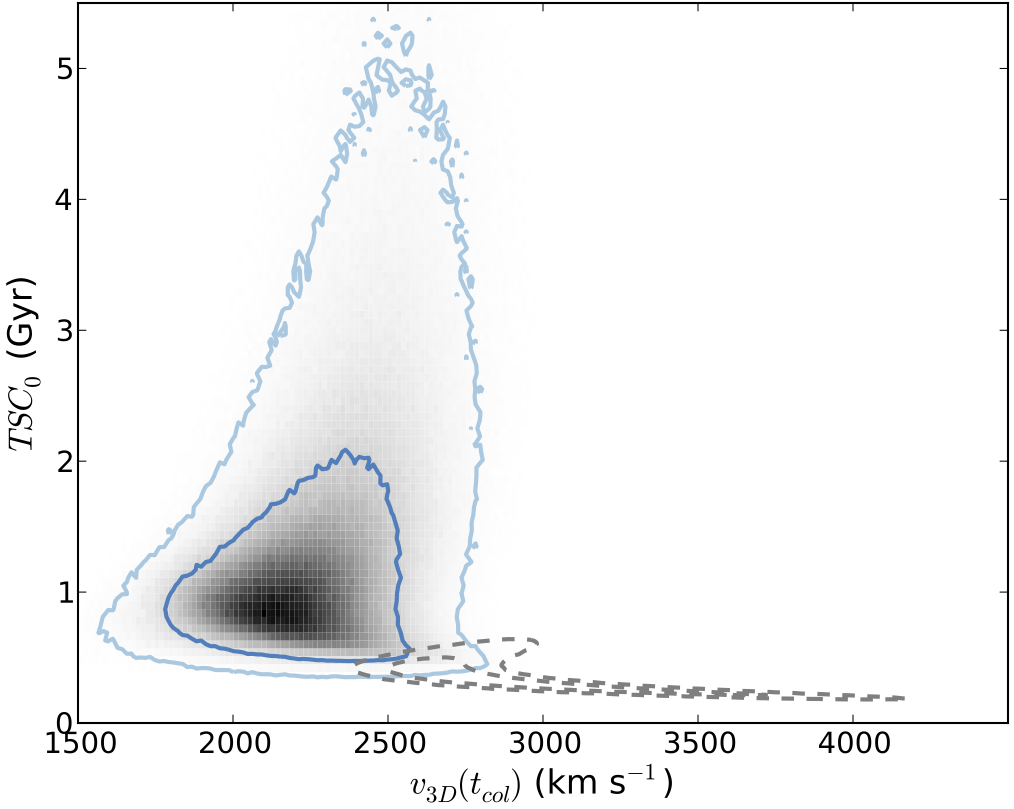
\includegraphics{Chapter3/MusketTSCwithBullet.png}
\caption{
The posterior of the Musket Ball Cluster's $TSC_0$ and $v_{\rm 3D}(t_{\rm col})$ parameters is shown in grayscale with dark and light blue contours representing 68\% and 95\% confidence, respectively.
For comparison the gray dashed contours are the Bullet Cluster's 68\% and 95\% confidence intervals copied from Figure \ref{fig_bcTSC_added}.
The Musket Ball Cluster occupies a much different region of merger phase than the Bullet Cluster, having both a slower relative collision velocity and being observed in a much later stage of merger.
\label{fig_mbc_TSC}}
\end{figure}

\begin{figure}
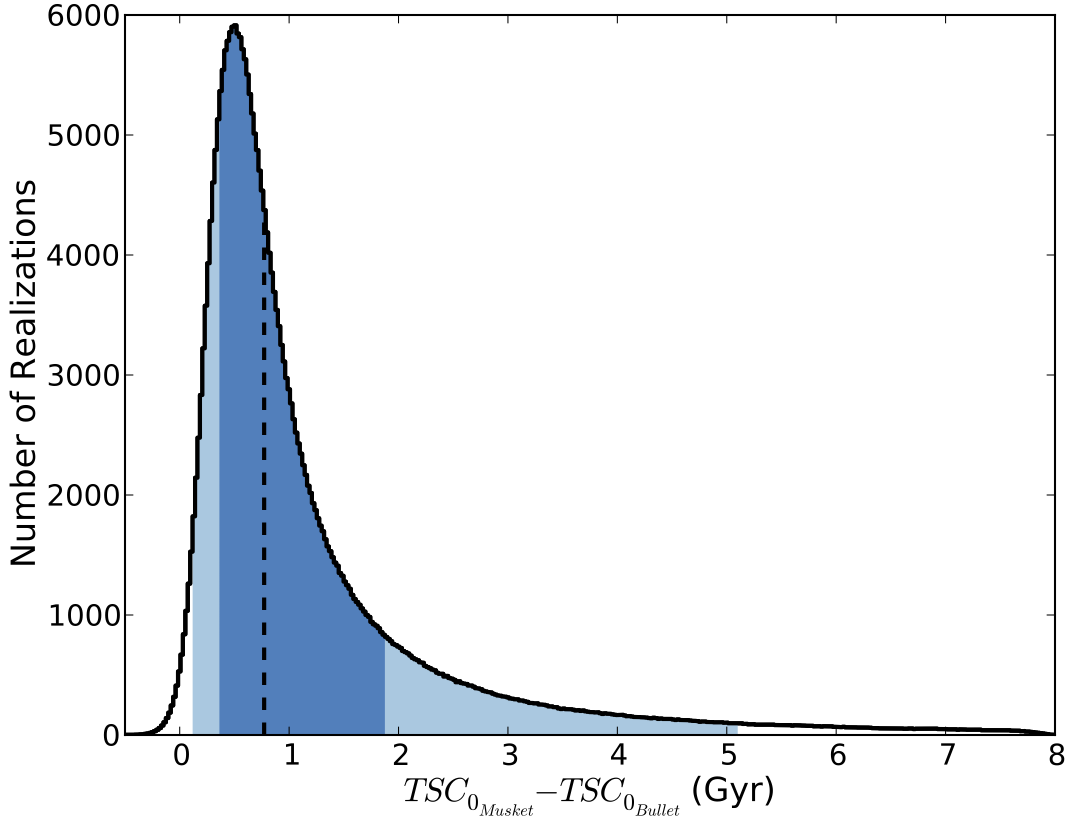
\includegraphics{Chapter3/TSC0subtraction.png}
\caption{
The histogram presents the $TSC_{\rm 0_{Musket}}-TSC_{\rm 0_{Bullet}}$ distribution from random draws of the respective marginalized $TSC_0$ distributions; showing that the Musket Ball Cluster merger is at least $0.8^{+1.2}_{-0.4}$\,Gyr ($3.4^{+3.8}_{-1.4}$ times) further progressed than the Bullet Cluster merger.
The black dashed line is the biweight-statistic location \citep{Beers:1982dp}, the 
dark and light blue regions denote the bias-corrected  68\% and 95\% lower and upper confidence limits, respectively.
\label{fig_TSC0comparison}}
\end{figure}

\begin{deluxetable*}{lcccc}
\tablewidth{0pt}
%\tabletypesize{\scriptsize}
\tablecaption{Musket Ball Cluster parameter estimates\label{musketballresultparam}}

\tablehead{
\colhead{Parameter}     & \colhead{Units}  & \colhead{Location\tablenotemark{a}}  & \colhead{68\% LCL--UCL\tablenotemark{b}} & \colhead{95\% LCL--UCL\tablenotemark{b}}
}
\startdata
M$_{200_1}$	&	$10^{14}$\,M$_\sun$	&	3.2	&	2.3	--	4.3	&	1.6	--	5.5	\\
M$_{200_2}$	&	$10^{14}$\,M$_\sun$	&	1.7	&	1.1	--	2.4	&	0.6	--	3.3	\\
$z_1$	&		&	0.5339	&	0.5333	--	0.5345	&	0.5326	--	0.5352	\\
$z_2$	&		&	0.5316	&	0.5305	--	0.5324	&	0.5294	--	0.5331	\\
$d_{\rm proj}$		&	Mpc	&	1.0	&	0.9	--	1.1	&	0.7	--	1.3	\\
$\alpha$	&	degree	&	48	&	28	--	67	&	13	--	78	\\
$d_{\rm 3D}$	&	Mpc	&	1.6	&	1.2	--	2.9	&	0.9	--	5.5	\\
$d_{\rm max}$	&	Mpc	&	2.1	&	1.5	--	3.8	&	1.1	--	7.3	\\
$v_{\rm 3D}(t_{\rm obs})$	&	km\,s$^{-1}$	&	670	&	390	--	1100	&	140	--	1500	\\
$v_{\rm 3D}(t_{\rm col})$ &	km\,s$^{-1}$	&	2300	&	2000	--	2500	&	1800	--	2800	\\
$TSC_0$	&	Gyr	&	1.1	&	0.7	--	2.4	&	0.5	--	5.8	\\
$TSC_1$\tablenotemark{c}	&	Gyr	&	3.5	&	2.0	--	7.2	&	1.4	--	12.0	\\
$T$	&	Gyr	&	4.8	&	2.9	--	10.4	&	2.2	--	22.7	\\
\enddata
\tablenotetext{a}{Biweight-statistic location \citep[see e.g.][]{Beers:1990kg}.}
\tablenotetext{b}{Bias-corrected lower and upper confidence limits, LCL and UCL respectively \citep[see e.g.][]{Beers:1990kg}.}
\tablenotetext{c}{61\% of the realizations with a valid $TSC_0$ (i.e.\,less than the age of the Universe at the cluster redshift) have a valid $TSC_1$, meaning that it is possible that the Musket Ball Cluster is being observed in the ``incoming'' state.}
\end{deluxetable*}

Note that just as a temporal prior was justified for the Bullet Cluster based on the observed shock front and increased temperature/mass estimate, I could apply a similar yet opposite prior to the Musket Ball since the temperature/mass estimate is consistent with the weak lensing inferred mass (additionally no shock front is observed).  
According to \citet{Randall:2002kk} if the cluster mass and inferred X-ray temperature or luminosity cluster mass are approximately the same then $TSC_0 \gtrsim 2 t_{\rm sc}$, which in the case of the Musket Ball means $TSC_0 \gtrsim 1.75$\,Gyr.
While this is consistent with my $TSC_0$ estimate for the Musket Ball, it is not entirely appropriate to apply this prior since the X-ray observations are relatively shallow and cannot confidently rule out a temperature and luminosity boost \citep{Dawson:2012dl}.
However it is conceivable that this line of reasoning would be applicable with deeper X-ray observations, either for the Musket Ball or similar dissociative mergers.

%\emph{Should I mention the fraction of realizations that have an allowable $TSC_1$, should I compare this with the Bullet cluster?}
 
\section{Summary and Discussion}\label{summary}

I have introduced a new method for determining the dynamic properties and associated uncertainty of dissociative cluster mergers given only the most general merger observables: mass of each subcluster, redshift of each subcluster, and projected separation the subclusters.
I find that this method addresses the primary weaknesses of existing methods, namely enabling accurate parameter estimation and propagation of uncertainty near the collision state with a convergent solution achieved in $\sim$6\,CPU\,hours. 
I have confirmed that the two NFW halo model is capable of achieving the required 10\% level accuracy by direct comparison with an N-body hydrodynamic simulation.

In applying this method to the Bullet Cluster I not only determined its merger dynamic parameters but found that the bulk of uncertainty in these parameters is due to uncertainty in $\alpha$, the angle of the merger with respect to the plane of the sky.
Analyses that fail to account for the uncertainty in $\alpha$ (all existing N-body simulations of the Bullet Cluster) will significantly underestimate the uncertainty in their results.
This highlights the need to carefully select and model many possible realizations of the merger when trying to infer results from N-body simulations of a real merger (I discuss this further in \S\ref{sec_suggestions}).
I have also shown how ex post facto priors can easily be applied to the results of the default priors to further constrain the inferred dynamic properties.
In particular accurate measurement of the cluster gas properties can enable approximately a factor of two better constraint on the dynamic properties of the merger, principally through added constraint on the time scale of the merger.

I have also applied this method to the Musket Ball Cluster, validating the approximate results of \citet{Dawson:2012dl}.
Comparing the dynamic properties of the Musket Ball with those of the Bullet I have shown that the Musket Ball represents a significantly different volume of merger phase space.
The Musket Ball Cluster, being $3.4^{+3.8}_{-1.4}$ times further progressed than the Bullet Cluster, could potentially provide tighter constraints on $\sigma_{\rm DM}$ since the offset between galaxies and dark matter should initially increase with time post-merger for  $\sigma_{\rm DM}>0$.
And the larger the expected offset, the better the dark matter constraint when applying a method similar to \citet{Randall:2008hs}.

\subsection{Suggested Uses of Method}\label{sec_suggestions}

While a general method for determining the dynamics properties of merging clusters has numerous applications, several are worth noting.
As noted N-body simulations of specific merging clusters are computationally expensive; in particular one SIDM simulation of a single dissociative merger requires $\sim$1--10 million CPU\,hours (private communication, James Bullock). 
Thus it is currently unfeasible to simulate all confirmed dissociative mergers.
This method can be used to quickly determine which mergers provide the best $\sigma_{\rm DM}$ constraining power, enabling an efficient use of limited computational resources.

Additionally it is inappropriate to simply simulate one realization of a dissociative merger due to the broad range of merger phase space allowed by uncertainty in observed parameters, as discussed in detail in \S\ref{sec_defaultprior}.
Thus multiple simulations of each merger are required to properly represent the allowed phase space.
One could conceivably reduce the number of required simulations by using the results of this method to select representative merger realizations that uniformly sample the merger phase space of interest (e.g. cluster mass, $v_{\rm 3D}(t_{\rm col})$, and $TSC_0$);
then weight the results of each simulated realization by the integral of the corresponding local phase space PDF, as determined by this method.
For example, one could estimate the uncertainty distribution of the $\sigma_{\rm DM}$ constraint inferred from SIDM simulations of the Bullet Cluster by weighting the constraint from each realization, where a realization with  $v_{\rm 3D}(t_{\rm col})$=2800\,km\,s$^{-1}$ and $TSC_0$=0.4\,Gyr would receive greater weight than one with $v_{\rm 3D}(t_{\rm col})$=4000\,km\,s$^{-1}$ and $TSC_0$=0.2\,Gyr, see Figure \ref{fig_bcTSC_added}.
Thus the results of this method will not only inform efficient selection of realizations to model but will reduce the number of simulations required to properly sample the posterior PDF's.
Nevertheless SIDM simulations of mock clusters need to be performed to determine how much acceptable values of $\sigma_{\rm DM}$ affect the inferred merger dynamics properties.

General merger dynamic properties are also important for understanding  how cluster mergers relate to other physical phenomena, such as galaxy evolution and radio relics.  
It is well established that galaxy clusters play an important role in the evolution of their member galaxies, but it is still unclear whether cluster mergers trigger star formation \citep[e.g.][]{Miller:2003kx,Owen:2005dx,Ferrari:2005es,Hwang:2009ip}, quench it \citep{Poggianti:2004ca}, or have no immediate effect \citep{Chung:2010ds}.
Studying mergers at different $TSC$ may resolve these seemingly conflicting results by  discriminating between slow-working processes (e.g.\,galaxy harassment or strangulation) and fast-acting process (e.g.\,ram pressure stripping). 
Similarly, studying global merger dynamic properties may resolve the mystery of why many mergers have associated radio relics \citep[e.g.][]{Barrena:2009to, vanWeeren:2011ko} yet others don't \citep[e.g.][]{Russell:2011hn}.

\subsection{Extensions to the Method}\label{sec_extensions}

While this method has advantages over existing methods there is room for considerable improvement.
For example the method could be improved through the elimination of some of the simplifying assumptions of the model (see \S\ref{sec_model}).
One could attempt to incorporate subcluster mass accretion physics in a manner similar to the work of \citet{Angus:2007em} or attempt to account for the possibility of a non-zero impact parameter.
To incorporate the latter one must: 1) add angular momentum terms to the equations of motion,  which is entirely feasible, and 2) prescribe a reasonable impact parameter prior.
\citet{Randall:2002kk} nicely outline how to determine an impact parameter PDF for halo mergers of variable mass by utilizing the PDF of the dimensionless \emph{spin parameter}, determined from linear theory of the growth of structure \citep{Peebles:1993vp} and simulations \citep{Bullock:2001kb}.
However, this prior should be adjusted to account for the samount of gas dissociated during the observed merger, since this amount will decrease as the impact parameter increases.
Without a systematic study of various mergers in hydrodynamic simulations it is unclear exactly what adjustment an observed large dissociation of gas should infer.

Another significant extension to the model could be the inclusion of SIDM physics.  
As mentioned in the previous section, one of the promising uses of this method is to suggest which mergers might provide the best $\sigma_{\rm DM}$ constraining power.  
However one could take this a step further by including an analytic treatment of SIDM physics \citep[e.g.\,][]{Markevitch:2004dl}, thereby enabling analytic estimates of $\sigma_{\rm DM}$ relevant effects for a given merger.
Then this method could be used in conjunction with observed dissociative mergers to place direct constraints on $\sigma_{\rm DM}$.
Due to the increased complexity of the physics involved
it would be necessary to verify this extension with SIDM N-body simulations.

%The addition of more informed priors offer an immediate extension to the model which does not require any actual changes to the model.
%For example, a mass function \citep[e.g.\,][]{Press:1974jb} based prior 


\emph{Note:} W. Dawson has made Python code implementing the discussed Monte Carlo method openly available at git://github.com/MCTwo/MCMAC.git.
He has also made all supporting work to this paper openly available at 
git://github.com/wadawson/merging-cluster-dynamics-paper.git.

\acknowledgments

I thank my adviser David Wittman who has always encouraged my research-freewill, while at the same time providing invaluable input and correcting guidance.
Our many fruitful discussions have touched every aspect of this work.
I also thank the Deep Lens Survey --- in particular Perry Gee --- for access to the 2007 Keck LRIS spectra, as well as Perry Gee and Brian Lemaux for assistance in reduction of the 2011 Keck DEIMOS spectra.  
I am grateful to  Jack P.\,Hughes for discussions on constraining the Bullet Cluster's TSC by the observed X-ray shock feature and boosted temperature/luminosity, and
Reinout J.\,van Weeren for discussions on the possibilities of constraining the dynamics and geometry of mergers using radio relics.
Finally I would like to thank Maru{\v s}a Brada{\v c}, Ami Choi, James Jee, Phil Marshall, Annika Peter, Michael Schneider, Reinout van Weeren, and David Wittman for their substantial reviews of earlier drafts.

Support for this work was provided by NASA through Chandra Award Number GO1-12171X issued by CXO Center, which is operated by the SAO for and on behalf of NASA under contract NAS8-03060.  Support for program number GO-12377 was provided by NASA through a grant from STScI, which is operated by the Association of Universities for Research in Astronomy, Inc., under NASA contract NAS5-26555.
Support for this work was also provide by Graduate Research Fellowships through the University of California, Davis.
I would also like to acknowledge the sultry universe who hides her secrets well.

%% See the AASTeX Web site at http://www.journals.uchicago.edu/AAS/AASTeX
%% for information on obtaining the facility keywords.

This work made use of the following facilities: CXO (ACIS-I), HST (ACS), Keck:I (LRIS), Keck:2 (DEIMOS), Mayall (MOSAIC 1 \& 1.1), Subaru (Suprime-Cam), SZA.

%% Appendix material should be preceded with a single \appendix command.
%% There should be a \section command for each appendix. Mark appendix
%% subsections with the same markup you use in the main body of the paper.

\clearpage

\appendix
%\section{Analysis Workflow Diagram}\label{workflowdiagram}
%
%The following is the programmatic workflow diagram of the Monte Carlo method discussed in \S\ref{sec_method}. 
%Random realizations of the merger will be drawn from input distributions of the subclusters' mass, $M_j$, redshift, $z_j$, and projected separation, $d_{\rm proj}$, where $j$ refers to either halo 1 or 2.
%The input distributions can be either Gaussian, with mean $\mu$ and standard deviation $\sigma$, or of more general form, perhaps as determined by previous bootstrap analyses.
%Merger dynamic parameters are calculated for each realization.
%Realizations with non-zero probability, as determined from priors, are stored and used to construct the merger parameter PDF's.
%The Monte Carlo analysis continues until the user defined number, $N_{\rm mc}$, of valid realizations have been analyzed.
% 
%
%\begin{figure}[b]
%\epsscale{1.}
%\figurenum{8}
%\plotone{TSM_top_revB.eps}
%\end{figure}
%
%\begin{figure}
%\epsscale{1.}
%\plotone{TSM_bottom_revB.eps}
%\setcounter{figure}{8}
%\caption{Programmatic workflow diagram of the Monte Carlo method discussed in \S\ref{sec_method}.
%Parameter notation is as defined in \S\ref{sec_method}.}
%\label{fig_flowchart}
%\end{figure}
%
%\clearpage
\section{Potential Energy of Two Truncated NFW Halos}\label{potentialsec}

Generically the potential energy of a two-halo system with center to center separation $r$ is 
\begin{equation}
V(r) = \int \Phi_1(r') dm_2,
\label{potint}
\end{equation}
where $\Phi_1(r')$ is the gravitational potential of halo 1 as a function of radial distance $r'$ from the center of the halo 1 to the mass element of halo 2, $dm_2$.  
I derive $\Phi_1(r)$ for the case of a truncated NFW halo in \S \ref{nfwpotential}.
The integral of equation \ref{potint} can be approximated as a summation over $N \times N$ mass elements, $m_{2_{ij}}$, each with area $dr\times d\theta$, where $i$ and $j$ range from $0 \rightarrow N-1$,
\begin{displaymath}
V(r) \approx \sum_{i=0}^{N-1}\sum_{j=0}^{N-1} \Phi_1(r'_{ij}+\epsilon) m_{2_{ij}},
\end{displaymath}
where $r'_{ij}$ is the distance from the center of halo 1 to the 2$^{\rm nd}$ halo's mass element $m_{2_{ij}}$, as derived in \S\ref{masselements}, and $\epsilon$ is the softening length which reduces the effects of artificial singularities.

\subsection{Truncated NFW Gravitational Potential}\label{nfwpotential}

For an axially symmetric mass distribution the potential can be expressed as a series of Legendre Polynomials

\begin{equation}
\Phi_n(r) = -\frac{2\pi G}{(n+1/2)r^{n+1}} \int_{0}^{r} r'^{n+2} \rho_{n}(r')\,dr' -\frac{2\pi G r^n}{n+1/2} \int_{r}^{\infty} r'^{1-n} \rho_n(r')\,dr' 
\label{axsympot}
\end{equation}
where
\begin{equation}
\rho_n(r) = (n+1/2) \int_{0}^{\pi} \rho(r,\theta) P_n(\cos \theta) \sin \theta \,d\theta.
\label{lengden}
\end{equation}

Assuming a spherical NFW halo
\begin{displaymath}
\rho_{\rm NFW}(r) = \frac{\rho_s}{r/r_s(1+r/r_s)^2}
\end{displaymath}
only the zero$^{\rm th}$ order term of Equation \ref{lengden} remains
\begin{displaymath}
\rho_{\rm NFW}(r) = \rho_0(r)
\end{displaymath}
and Equation \ref{axsympot} reduces to
\begin{eqnarray}
\Phi_{\rm NFW}(r) & = & -\frac{4\pi G}{r}\int_{0}^{r} r'^2 \rho_{\rm NFW}(r')\,dr' - 4\pi G \int_{r}^{\infty}r' \rho_{\rm NFW}(r')\,dr' \nonumber\\
\Phi_{\rm NFW}(r) & = & -\frac{4\pi G \rho_s}{r} \left[ \int_{0}^{r} \frac{r'^2}{r'/r_s(1+r'/r_s)^2}\,dr' + r \int_{r}^{\infty} \frac{r'}{r'/r_s(1+r'/r_s)^2}\,dr' \right]. \nonumber
\end{eqnarray}
Since I truncate the NFW halo at $r_{200}$ the $\infty$ in the second integral becomes $r_{200}$ and
\begin{equation}
	\Phi_{\rm NFW_T}(r)=
	\begin{cases}
 		-\frac{4\pi G}{r} \rho_s r_s^3 \left[ \ln (1+r/r_s)-\frac{r}{r_s+r_{200}} \right], &\text{if $r\leq r_{200}$;}\\
  		-\frac{G M_{200}}{r}, &\text{if $r>r_{200}$.}
  	\end{cases}
\end{equation}

\subsection{Mass Elements of a Truncated NFW Halo}\label{masselements}

Given the differential mass elements for a spherically symmetric halo
\begin{displaymath}
dm = 2\pi\rho(r,\theta) r^2 \sin(\theta) d\theta\,dr,
\end{displaymath}
and discretizing the mass into elements with lengths $\delta r = r_{200_2}/N$ and $\delta\theta = \pi/N$ the halo 2 mass elements are given by
\begin{displaymath}
m_{ij} = 2\pi \int_{i\,\delta r}^{(i+1)\delta r} \int_{j\,\delta\theta}^{(j+1)\delta\theta} \rho(r') r'^2 \sin(\theta') d\theta'\,dr'.
\end{displaymath}
For an NFW halo this becomes
\begin{displaymath}
m_{ij} = 2\pi\rho_s r_s^3 \left[\cos(j\,\delta\theta)-\cos\left((j+1)\delta\theta\right) \right] \left[ \left( 1+\frac{(i+1)\delta r}{r_s}\right)^{-1} - \left(1+\frac{i\,\delta r}{r_s}\right)^{-1} + \ln\left[\frac{(i+1)\delta r+r_s}{i\,\delta r+r_s}\right]\right].
\end{displaymath}

\clearpage

\section{Musket Ball Cluster Redshift Catalog}\label{sec_MBCzcat}

The Musket Ball Cluster redshift catalog (Table \ref{table_MBCzcat}) contains 738 spectroscopically confirmed galaxy redshifts.  The galaxies are within an $\sim 18\arcmin \times 18\arcmin$ area centered on the Musket Ball Cluster ($139.05\deg$, $+29.85\deg$).  The source of the redshifts are from three separate spectroscopic surveys: 1) \emph{LRIS 2007} was carried out on 2007 January 15 using the Keck:I LRIS instrument, 2) \emph{DEIMOS 2011A} was carried out on 2011 March 1 \& 2 using the Keck:II DEIMOS instrument, and 3) \emph{DEIMOS 2012B} was carried out on 2013 January 16 using the Keck:II DEIMOS instrument.

The \emph{DEIMOS 2011A} observations consisted of 6 slit masks  with 1\arcsec slits and using the 1200\,line\,mm$^{-1}$ grating, tilted to a central wavelentgh of 6700\,\AA, resulting in a pixel scale of 0.33\,$\AA$\,pixel$^{-1}$, a resolution of $\sim1.1$\,\AA (50\,km\,s$^{-1}$), and typical wavelength coverage of 5400\AA\,to 8000\AA. 
The \emph{DEIMOS 2013B} observations consisted of 1 slit mask with 1\arcsec slits and using the 1200\,line\,mm$^{-1}$ grating, tilted to a central wavelentgh of 6200\,\AA, resulting in a pixel scale of 0.33\,\AA\,pixel$^{-1}$, a resolution of $\sim1$\,\AA (50\,km\,s$^{-1}$), and typical wavelength coverage of 4900\AA\,to 7500\AA. 
The exposures for each DEIMOS mask ($\sim3\times20$\,minutes) were combined using the DEEP2 version of the spec2d package \citep{Newman:2012ta}.
This package combines the individual exposures of the slit mosaic and performs wavelength calibration, cosmic ray removal and sky subtraction on slit-by-slit basis, generating a processed two-dimensional spectrum for each slit. 
The spec2d pipeline also generates a processed one-dimensional spectrum for each slit.
This extraction creates a one-dimensional spectrum of the target, containing the summed flux at each wavelength in an optimized window. 
Table \ref{table_MBCzcat} only includes high quality (Q $\geq$ 3, see \citet{Newman:2012ta} for an explanation on the quality codes) galaxy spectra.
Details of the \emph{LRIS 2007} observations and reduction are discussed in the Deep Lens Survey data release paper (Wittman et al. in prep).

%% The values (usually only l,r and c) in the last part of
%% \begin{deluxetable}{} command tell LaTeX how many columns
%% there are and how to align them.
\begin{deluxetable}{cccccccc}

%% Keep a portrait orientation

%% Over-ride the default font size
%% Use 8pt
\tabletypesize{\scriptsize}

%% Use \tablewidth{?pt} to over-ride the default table width.
%% If you are unhappy with the default look at the end of the
%% *.log file to see what the default was set at before adjusting
%% this value.

%% This is the title of the table.
\tablecaption{Musket Ball Cluster Redshift Catalog\label{table_MBCzcat}}

%% This command over-rides LaTeX's natural table count
%% and replaces it with this number.  LaTeX will increment
%% all other tables after this table based on this number
\tablenum{4}

%% The \tablehead gives provides the column headers.  It
%% is currently set up so that the column labels are on the
%% top line and the units surrounded by ()s are in the
%% bottom line.  You may add more header information by writing
%% another line between these lines. For each column that requries
%% extra information be sure to include a \colhead{text} command
%% and remember to end any extra lines with \\ and include the
%% correct number of &s.
\tablehead{\colhead{RA} & \colhead{Dec} & \colhead{PosErr} & \colhead{z} & \colhead{$\sigma$z} & \colhead{Source} & \colhead{R } & \colhead{$\sigma$R} \\
\colhead{(hh:mm:ss.sss)} & \colhead{(dd:mm:ss.ss)} & \colhead{(arcsec)} & \colhead{} & \colhead{} & \colhead{} & \colhead{(mag)} & \colhead{(mag)} }
%% All data must appear between the \startdata and \enddata commands
\startdata
09:15:40.142 & +29:55:06.71 & 0.5 & 0.234777 & 0.000020 & DEIMOS 2011A & 20.983 & 0.007 \\
09:15:41.501 & +29:47:07.64 & 0.5 & 0.530381 & 0.000024 & DEIMOS 2011A & 23.398 & 0.048 \\
09:15:41.682 & +29:55:13.05 & 0.5 & 0.704062 & 0.000033 & DEIMOS 2011A & 22.586 & 0.024 \\
09:15:41.726 & +29:56:12.79 & 0.5 & 0.498200 & 0.000015 & DEIMOS 2011A & 22.664 & 0.016 \\
09:15:42.418 & +29:46:55.71 & 0.5 & 0.899342 & 0.000101 & DEIMOS 2011A & 22.246 & 0.017 \\
\enddata
%% Include any \tablenotetext{key}{text}, \tablerefs{ref list},
%% or \tablecomments{text} between the \enddata and
%% \end{deluxetable} commands

%% General table comment marker
\tablecomments{Table 4 is published in its entirety in the electronic
edition of the {\it Astrophysical Journal}.  A portion is shown here
for guidance regarding its form and content.}

%% No \tablerefs indicated

\end{deluxetable}

\clearpage

\section{Bullet Cluster Result Plots}\label{sec_bcresults}

This section contains the parameter results array plots for the Bullet Cluster case including the added temporal prior of \S\ref{sec_addedprior}.
For ease of display the parameters are grouped in three categories (\emph{Input}, \emph{Geometry}, and \emph{Velocity \& Time}) resulting in a six subplot results array, see Figure \ref{fig_resultsarray}.
The \emph{Input} parameters consist of: M$_{200_1}$, M$_{200_2}$, $z_1$, $z_2$,	and $d_{\rm proj}$, where halo 1 refers to the ``main'' subcluster and halo 2 refers to the ``bullet'' subcluster.
The \emph{Geometry} parameters consist of the randomly drawn $\alpha$, and calculated $d_{\rm 3D}$, and $d_{\rm max}$.
The calculated \emph{Velocity \& Time} parameters consist of:  $TSC_0$, $TSC_1$, and $T$.

\begin{figure}[b]
\includegraphics{Chapter3/ResultsArray_RevB.png}
\caption{
For ease of display the results array is divided into six subplots, Figures \ref{fig_bc_inin}--\ref{fig_bc_geovt}.
The Input parameters consist of: M$_{200_1}$, M$_{200_2}$, $z_1$, $z_2$,	and $d_{\rm proj}$.
The calculated Geometry parameters consist of: $\alpha$, $d_{\rm 3D}$, and $d_{\rm max}$.
The calculated Velocity \& Time parameters consist of:  $v_{\rm 3D}(t_{\rm obs})$, $v_{\rm 3D}(t_{\rm col})$, $TSC_0$, $TSC_1$, and $T$.
\label{fig_resultsarray}}
\end{figure}
\clearpage

\begin{figure}
\includegraphics{Chapter3/bullet_shockprior_input-input.png}
\caption{Bullet Cluster marginalized \emph{Input vs.\,Input} parameters result plots, for the case including the added temporal prior of \S\ref{sec_addedprior}. Dark and light blue colors correspond to 68\% and 95\% confidence intervals, respectively.  The black dashed line is the biweight-statistic location \citep{Beers:1982dp}. 
\label{fig_bc_inin}}
\end{figure}
%\clearpage

\begin{figure}
\includegraphics{Chapter3/bullet_shockprior_input-geometry.png}
\caption{Bullet Cluster marginalized \emph{Input vs.\,Geometry} parameters result plots, for the case including the added temporal prior of \S\ref{sec_addedprior}.  Dark and light blue colors correspond to 68\% and 95\% confidence intervals, respectively.
\label{fig_bc_ingeo}}
\end{figure}
%\clearpage

\begin{figure}
\includegraphics{Chapter3/bullet_shockprior_input-vt.png}
\caption{Bullet Cluster marginalized \emph{Input vs.\,Velocity \& Time} parameters result plots, for the case including the added temporal prior of \S\ref{sec_addedprior}.  Dark and light blue colors correspond to 68\% and 95\% confidence intervals, respectively.
\label{fig_bc_invt}}
\end{figure}
%\clearpage

\begin{figure}
\includegraphics{Chapter3/bullet_shockprior_geometry-geometry.png}
\caption{Bullet Cluster marginalized \emph{Geometry vs.\,Geometry} parameters result plots, for the case including the added temporal prior of \S\ref{sec_addedprior}.  Dark and light blue colors correspond to 68\% and 95\% confidence intervals, respectively.  The black dashed line is the biweight-statistic location \citep{Beers:1982dp}.
\label{fig_bc_geogeo}}
\end{figure}
%\clearpage

\begin{figure}
\includegraphics{Chapter3/bullet_shockprior_geometry-vt.png}
\caption{Bullet Cluster marginalized \emph{Geometry vs.\,Velocity \& Time} parameters result plots, for the case including the added temporal prior of \S\ref{sec_addedprior}.  Dark and light blue colors correspond to 68\% and 95\% confidence intervals, respectively.
\label{fig_bc_geovt}}
\end{figure}
%\clearpage

\begin{figure}
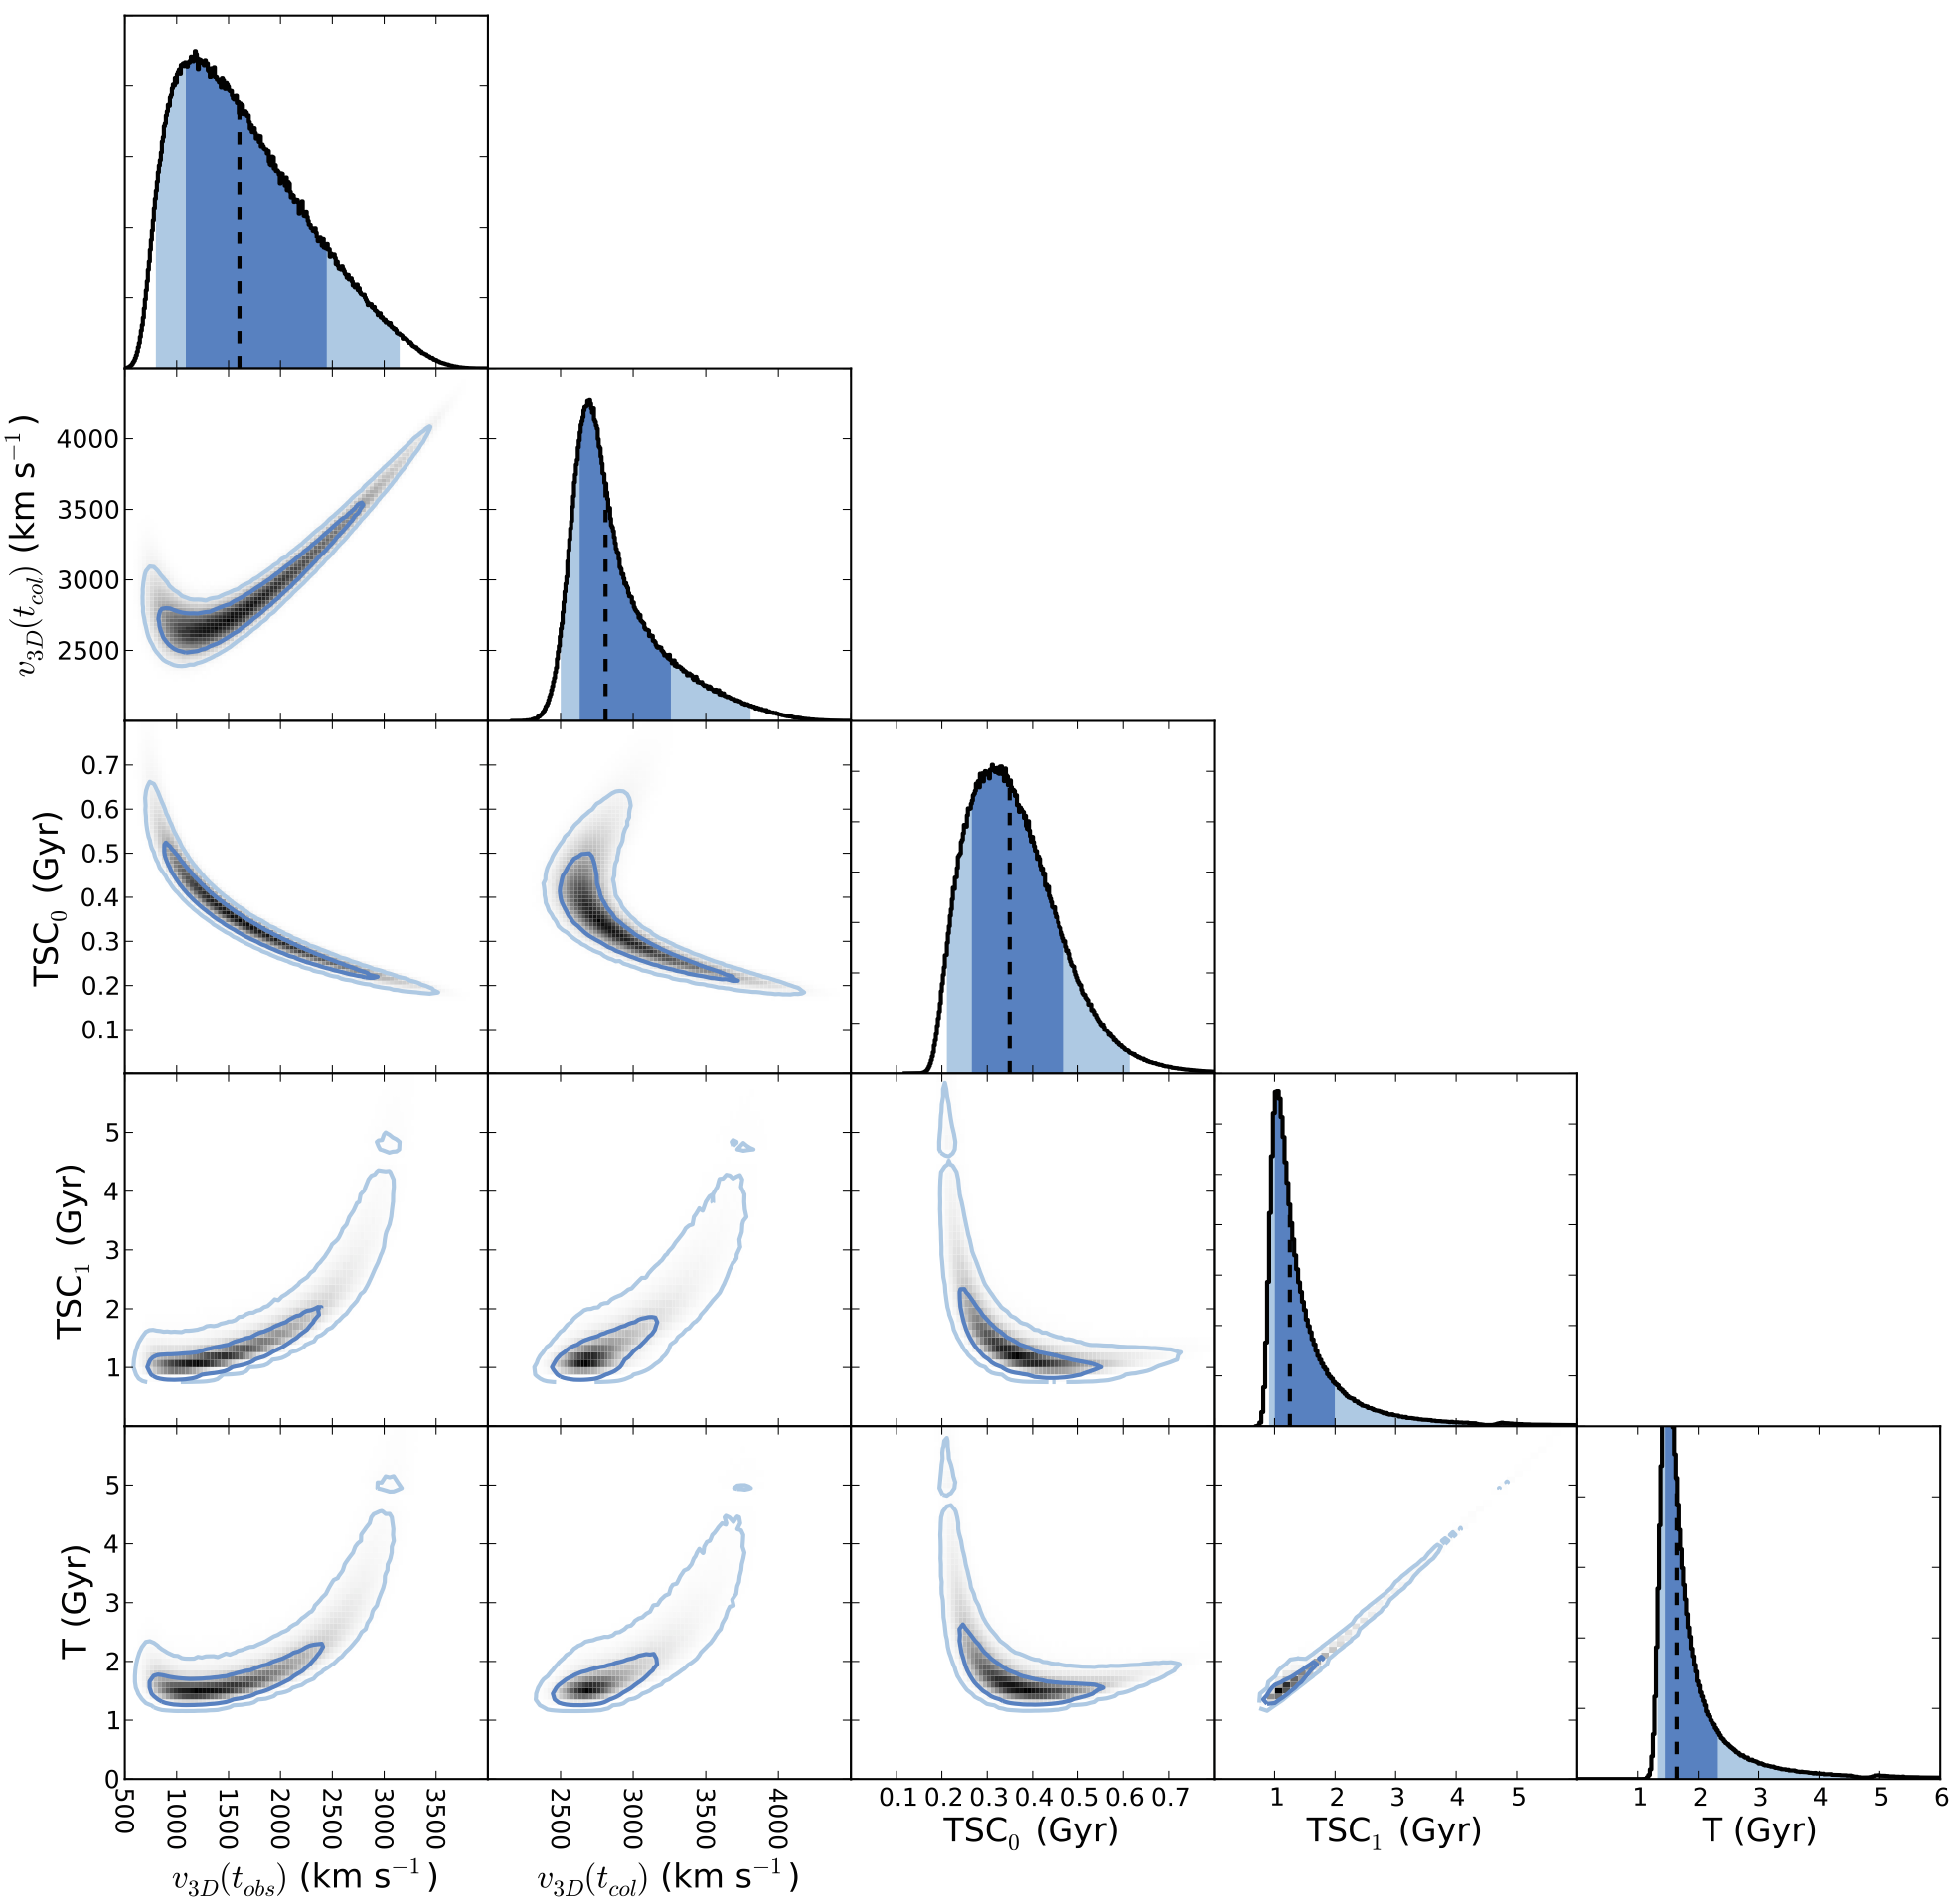
\includegraphics{Chapter3/bullet_shockprior_vt-vt.png}
\caption{Bullet Cluster marginalized \emph{Velocity \& Time vs.\,Velocity \& Time} parameters result plots, for the case including the added temporal prior of \S\ref{sec_addedprior}.  Dark and light blue colors correspond to 68\% and 95\% confidence intervals, respectively.  The black dashed line is the biweight-statistic location \citep{Beers:1982dp}.
\label{fig_bc_vtvt}}
\end{figure}
\clearpage


\section{Musket Ball Cluster Result Plots}\label{sec_mbcresults}

This section contains the parameter results array plots for the Musket Ball Cluster.
Similar to \S\ref{sec_bcresults} the parameters are grouped in three categories (\emph{Input}, \emph{Geometry}, and \emph{Velocity \& Time}) resulting in a six subplot results array, see Figure \ref{fig_resultsarray}.
The \emph{Input} parameters consist of: M$_{200_1}$, M$_{200_2}$, $z_1$, $z_2$,	and $d_{\rm proj}$, where halo 1 refers to the ``south'' subcluster and halo 2 refers to the ``north'' subcluster.
The calculated \emph{Geometry} parameters consist of: $\alpha$, $d_{\rm 3D}$, and $d_{\rm max}$.
The calculated Velocity \& Time parameters consist of:  $v_{\rm 3D}(t_{\rm obs})$, $v_{\rm 3D}(t_{\rm col})$, $TSC_0$, $TSC_1$, and $T$.

\begin{figure}[b]
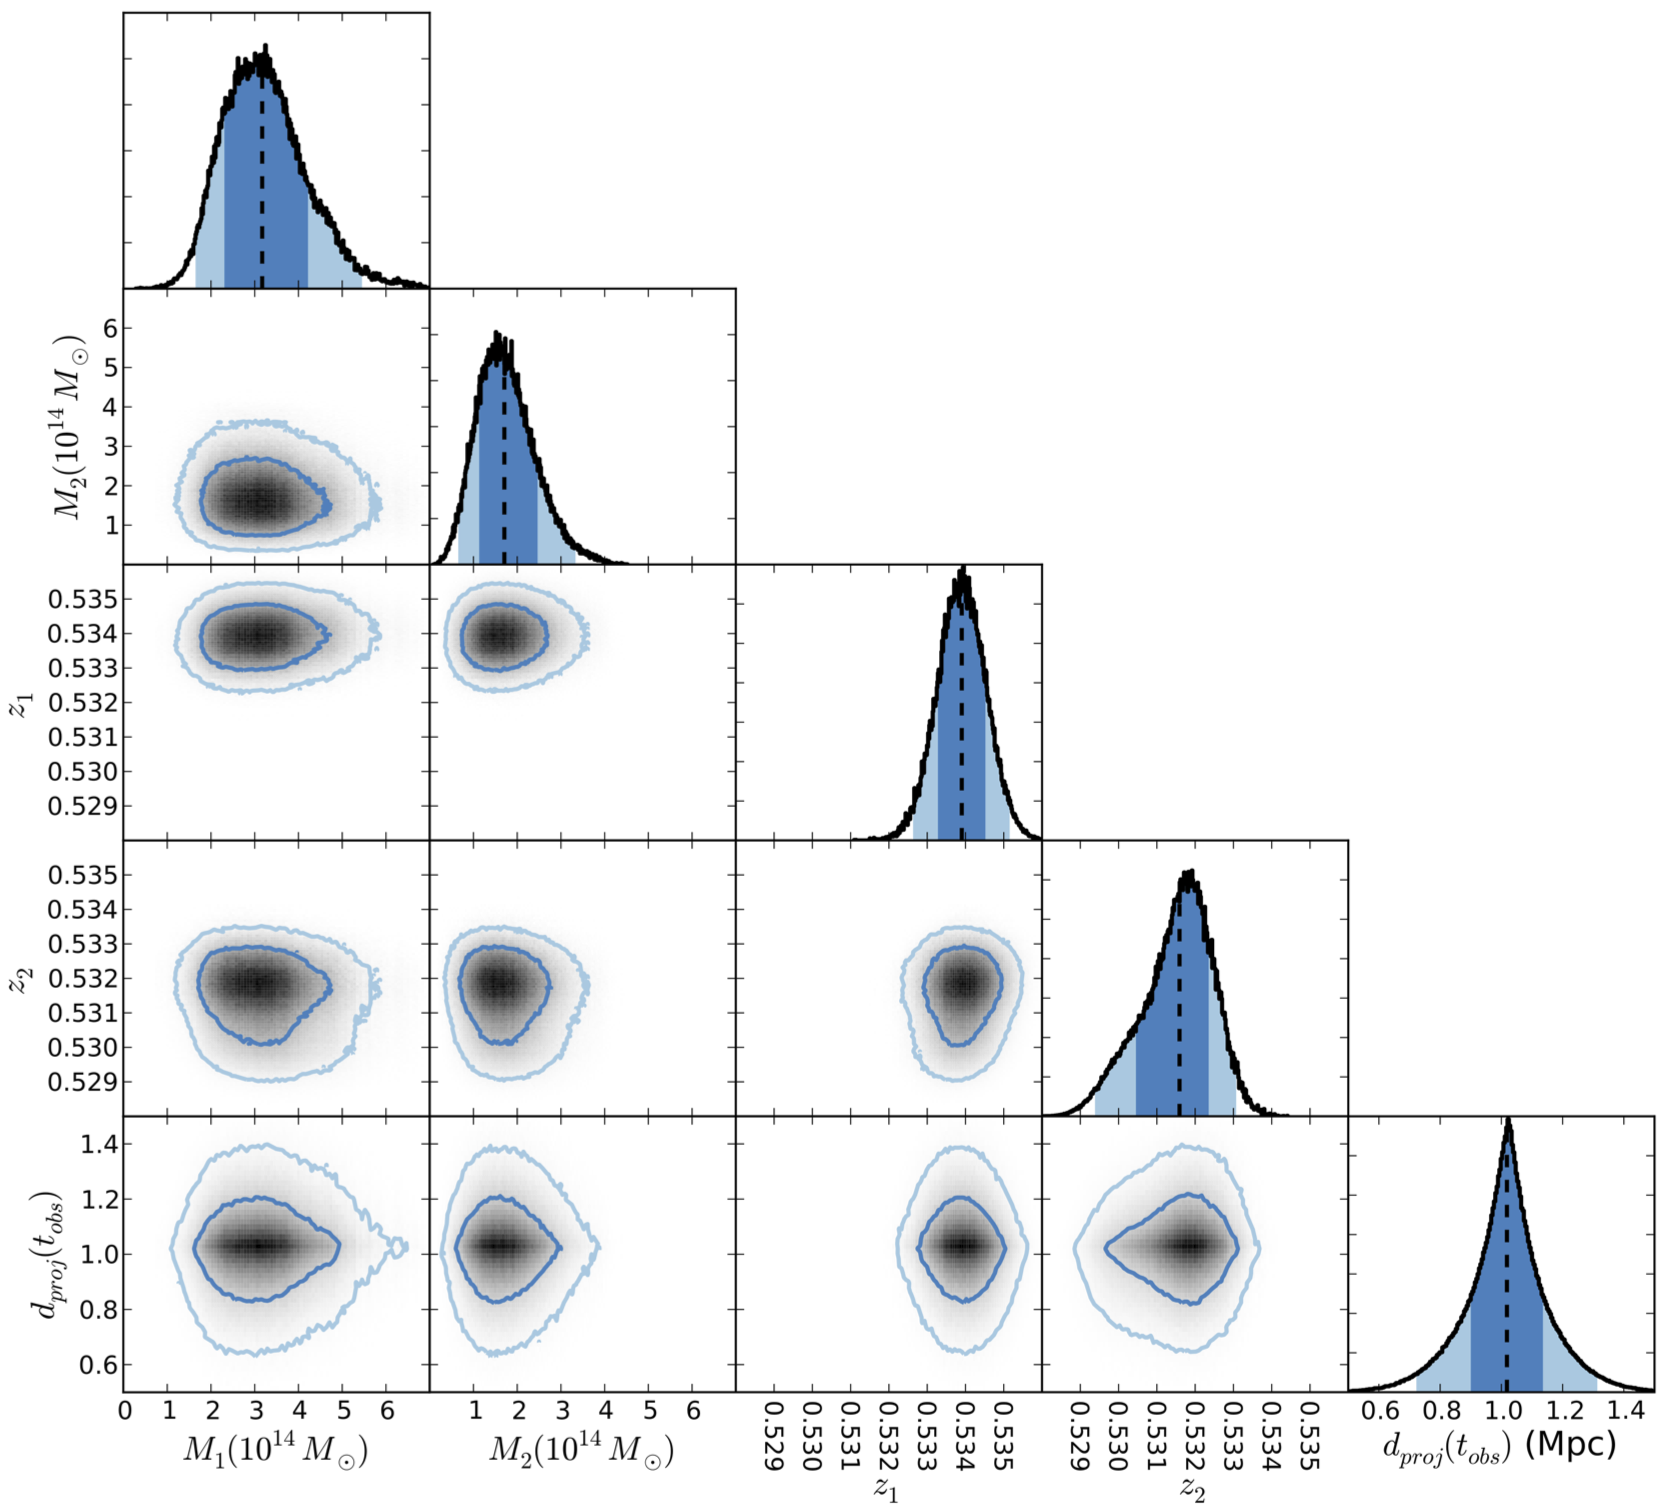
\includegraphics{Chapter3/run_v11_revB_input-input.png}
\caption{Musket Ball Cluster marginalized \emph{Input vs.\,Input} parameters result plots.  Dark and light blue colors correspond to 68\% and 95\% confidence intervals, respectively.  The black dashed line is the biweight-statistic location \citep{Beers:1982dp}.
\label{musket_inin}}
\end{figure}
%\clearpage

\begin{figure}
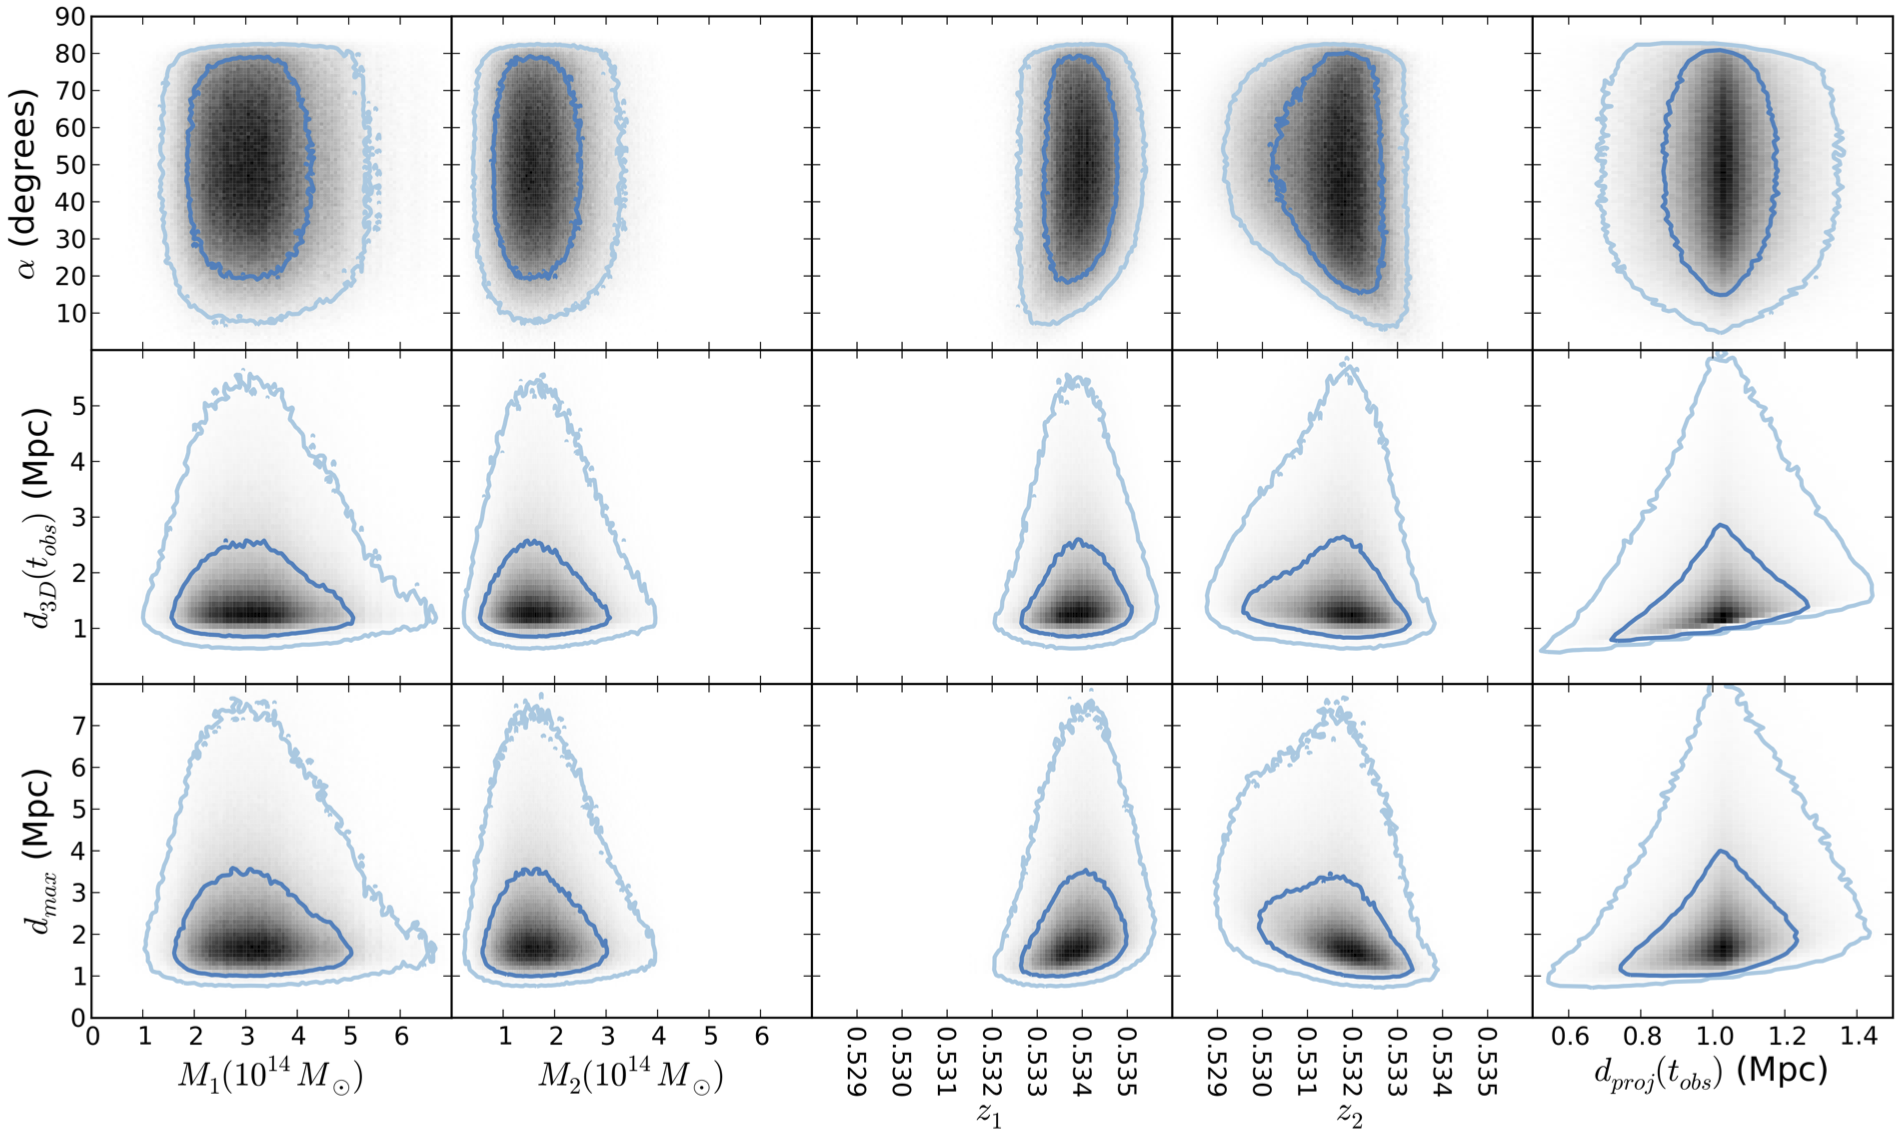
\includegraphics{Chapter3/run_v11_revB_input-geometry.png}
\caption{Musket Ball Cluster marginalized \emph{Input vs.\,Geometry} parameters result plots.  Dark and light blue colors correspond to 68\% and 95\% confidence intervals, respectively.
\label{musket_ingeo}}
\end{figure}
%\clearpage

\begin{figure}
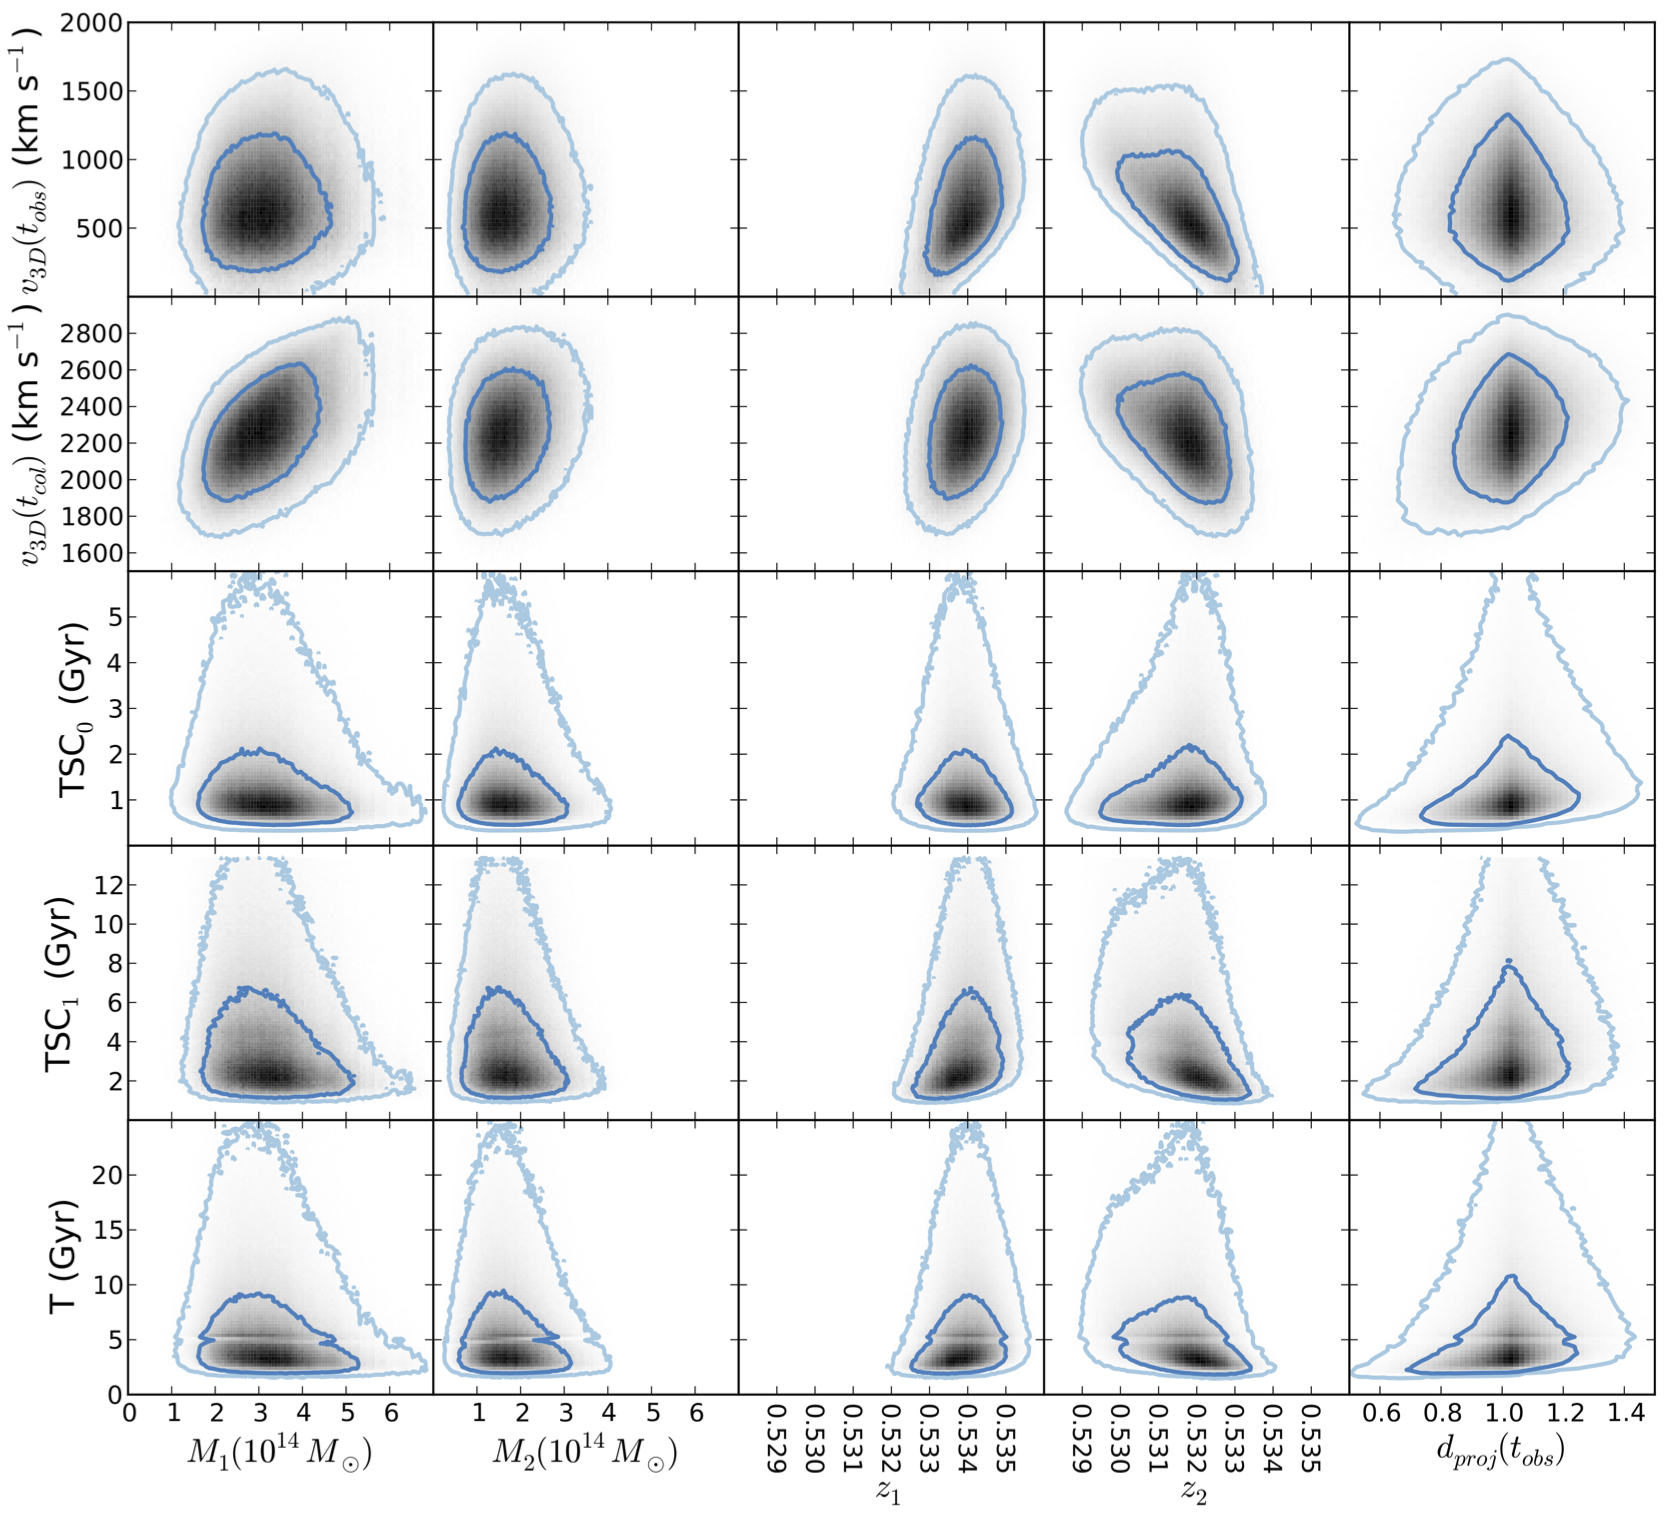
\includegraphics{Chapter3/run_v11_revB_input-vt.png}
\caption{Musket Ball Cluster marginalized \emph{Input vs.\,Velocity \& Time} parameters result plots.  Dark and light blue colors correspond to 68\% and 95\% confidence intervals, respectively.
\label{musket_invt}}
\end{figure}
%\clearpage

\begin{figure}
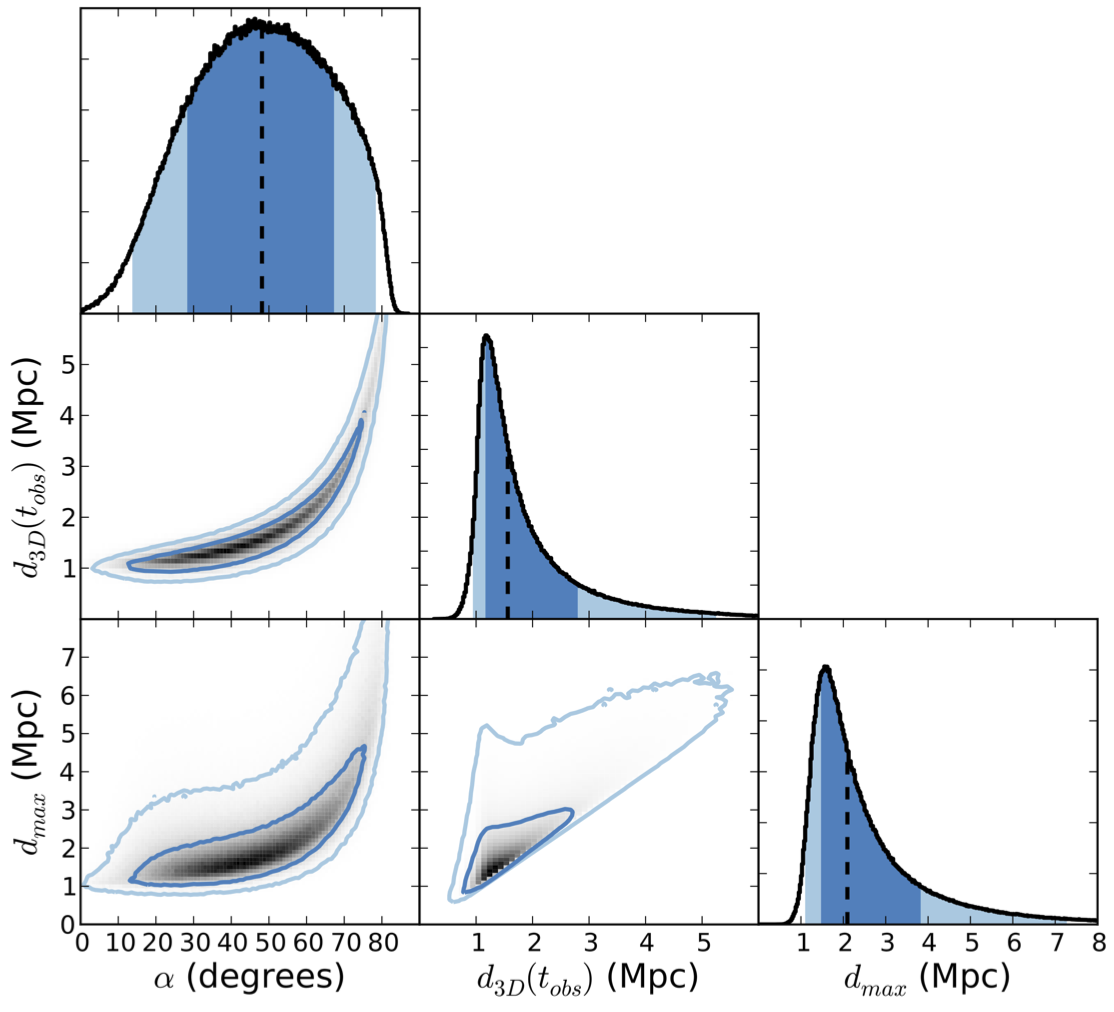
\includegraphics{Chapter3/run_v11_revB_geometry-geometry.png}
\caption{Musket Ball Cluster marginalized \emph{Geometry vs.\,Geometry} parameters result plots.  Dark and light blue colors correspond to 68\% and 95\% confidence intervals, respectively.  The black dashed line is the biweight-statistic location \citep{Beers:1982dp}.
\label{musket_geogeo}}
\end{figure}
%\clearpage

\begin{figure}
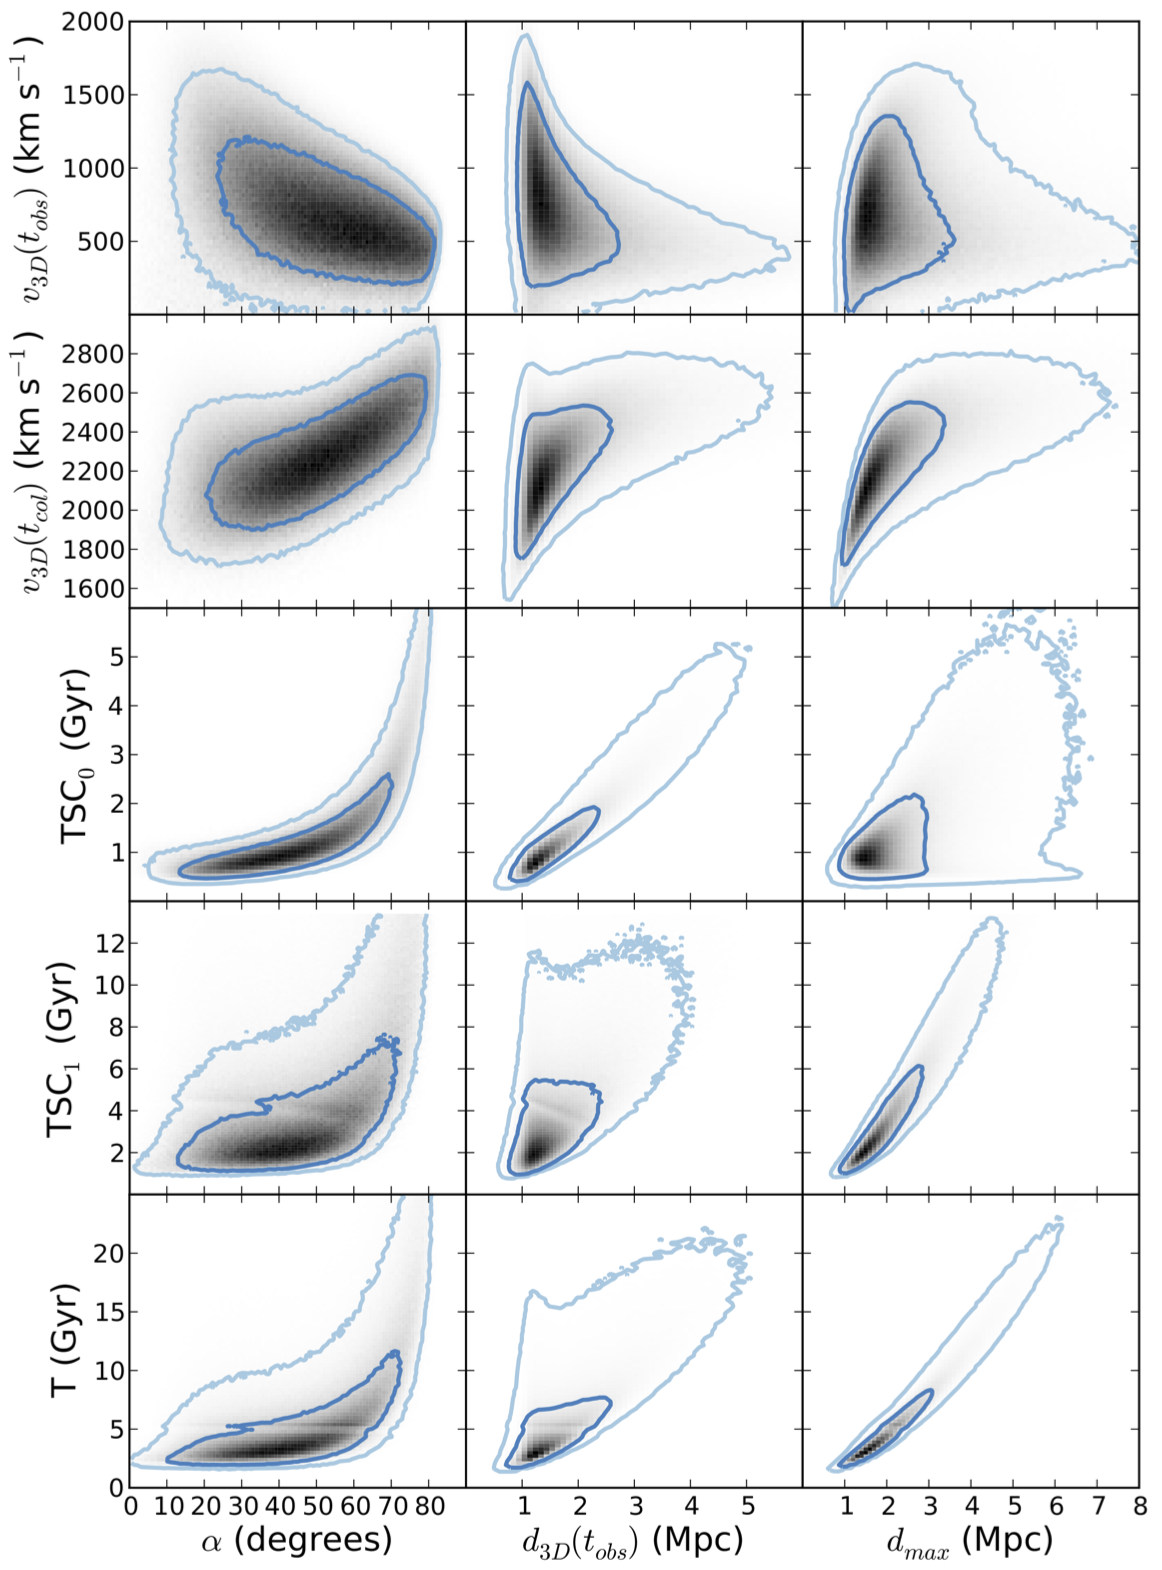
\includegraphics{Chapter3/run_v11_revB_geometry-vt.png}
\caption{Musket Ball Cluster marginalized \emph{Geometry vs.\,Velocity \& Time} parameters result plots.  Dark and light blue colors correspond to 68\% and 95\% confidence intervals, respectively.
\label{musket_geovt}}
\end{figure}
%\clearpage

\begin{figure}
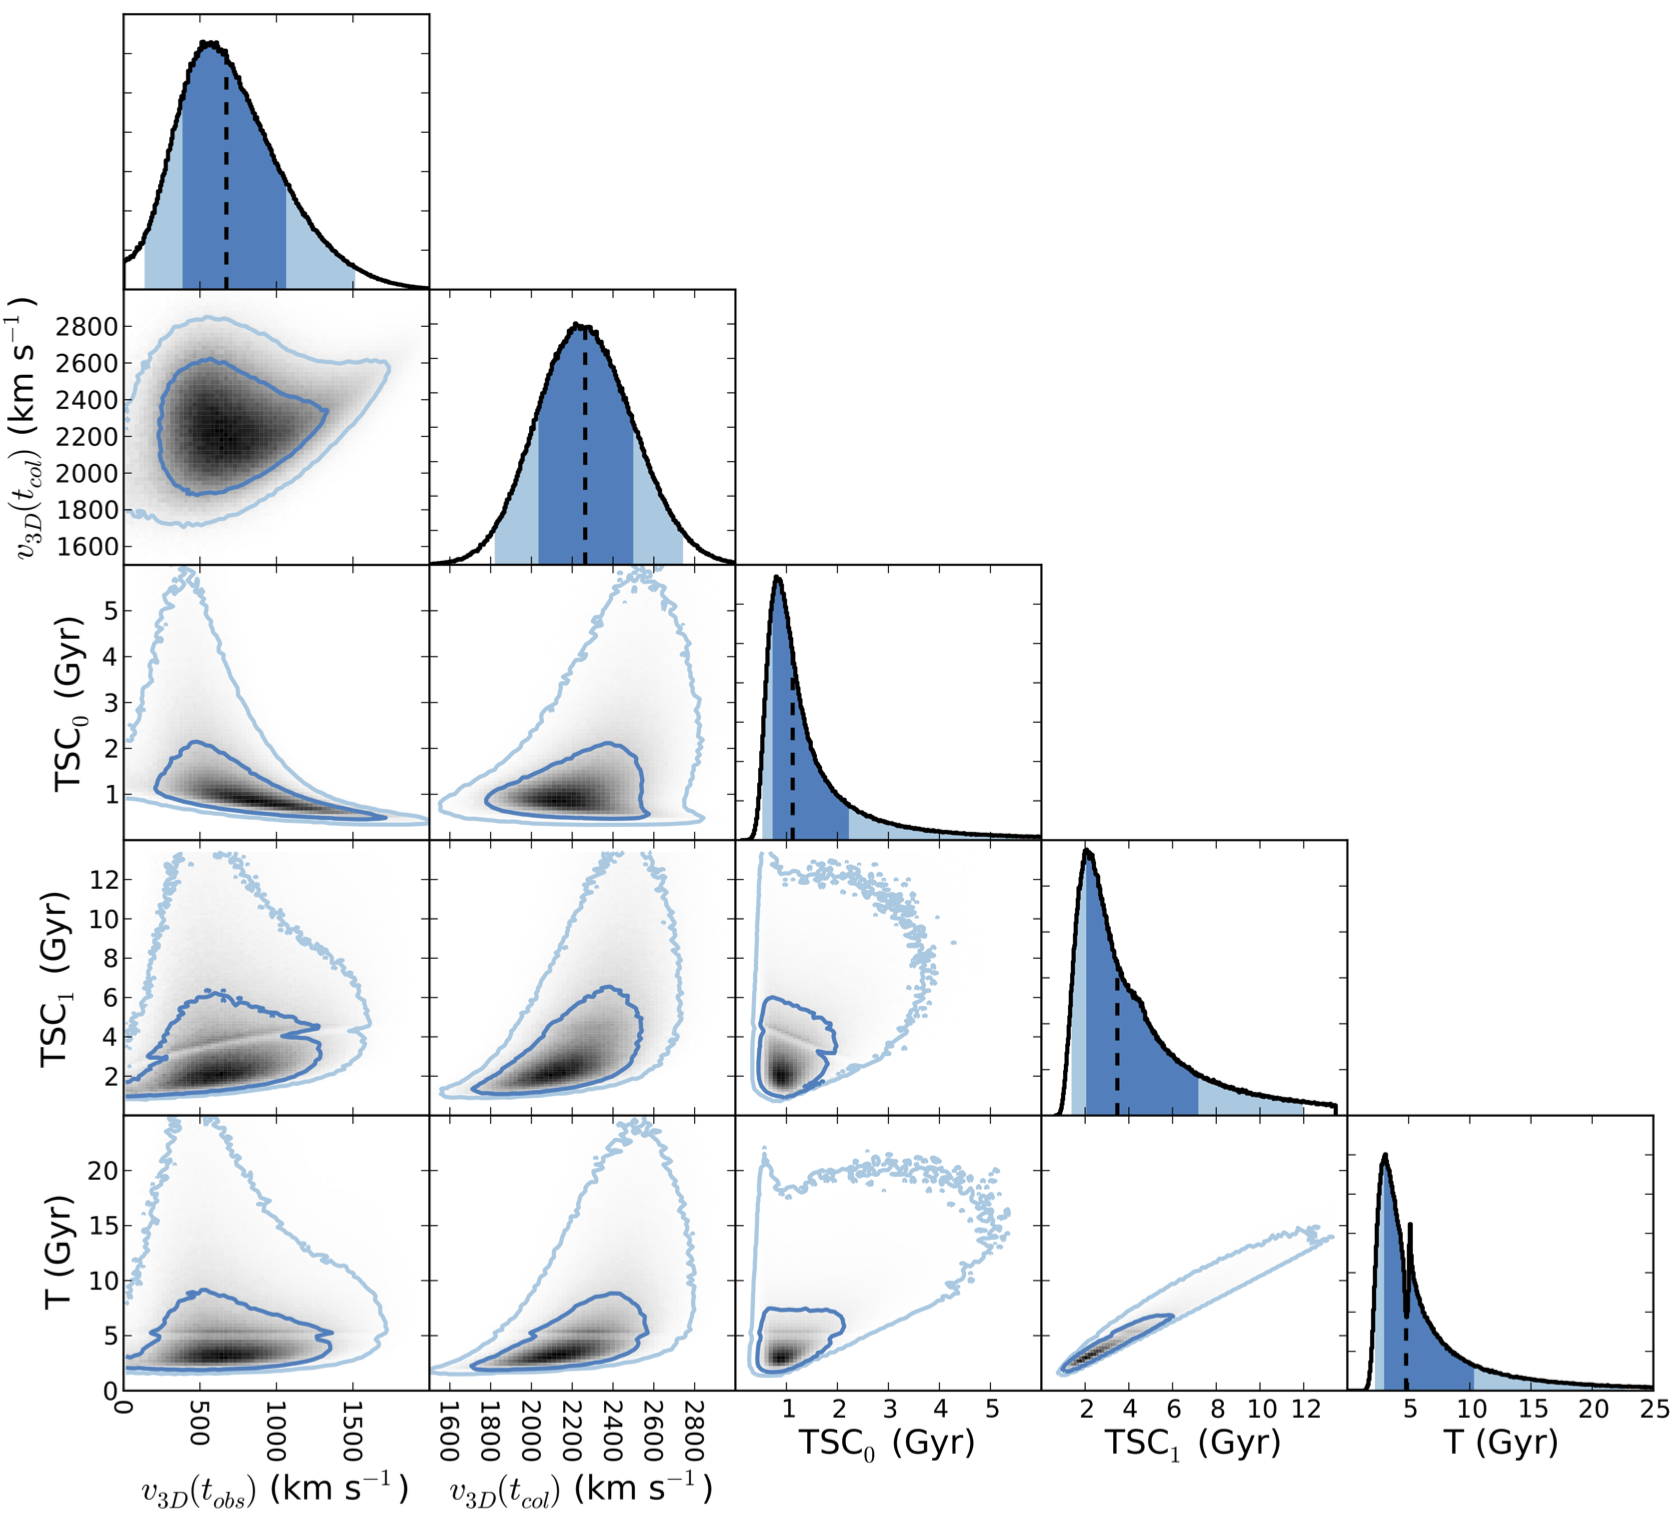
\includegraphics{Chapter3/run_v11_revB_vt-vt.png}
\caption{Musket Ball Cluster marginalized \emph{Velocity \& Time vs.\,Velocity \& Time} parameters result plots.  Dark and light blue colors correspond to 68\% and 95\% confidence intervals, respectively.  The black dashed line is the biweight-statistic location \citep{Beers:1982dp}.
\label{musket_vtvt}}
\end{figure}
        
    % %-----------------------------------------------------------------------
    % 
    % %-------------------------------------------------------- NEW CHAPTER --
    %
    % % -- Chapter 4

    \newchapter{Musket Ball: DM Implications}{Musket Ball Cluster: Dark Matter Implications}{Musket Ball Cluster: Dark Matter Implications}
\label{chapter:4}

\noindent Portions of this chapter were originally published in the article titled \emph{Discovery of a Dissociative Galaxy Cluster Merger with Large Physical Separation} which was published in the March 2012 issue of the Astrophysical Journal Letters (Volume 747, pp. L42). \\

\section{Introduction}

As introduced in \S\ref{section:DMconstraintWithMergers} there are four methods of constraining $\sigma_{\rm SIDM}$ with observations of dissociative mergers.
In this chapter we apply two of those methods to observations of the Musket Ball Cluster.
First we will consider the gas-DM offset, and second we will consider the galaxy-DM offset.
As discussed in \S\ref{section:DMconstraintWithMergers} these two methods are believed to be the most robust.
In both cases we will depend on the WL measurements to ascertain the location of the DM.
The galaxy location will be determined from optical spectroscopic and photometric observations of the galaxies.
The gas location will be determined from X-ray observations of the cluster.
Of the three location measurements... (the galaxy is the most difficult???)

We note that the exercise of comparing the galaxy-WL offset will be incomplete in this analysis, since simulations of mergers with varying $\sigma_{\rm SIDM}$ are necessary to turn any observed offset (or lack of offset) into a quantitative constraint on$\sigma_{\rm SIDM}$ (see \S\ref{section:DMgalaxyOffsetIntro}). 
However we chose to present the observation portion of this analysis for two reasons.
First, it is a necessary first step towards applying this constraint.
Secondly, if a significant offset is observed then one could still conclude that $\sigma_{\rm SIDM}$>0, which would be a significant finding since this would imply that DM is self-interacting via a new force.

For both the gas-DM offset and galaxy-DM offset methods the primary measurements necessary are the location of the galaxies (\S\ref{section:GalaxyLocation}), gas (\S\ref{section:GasLocation}), and DM (\S\ref{section:WLLocation}).
Much of this chapter will focus on how there measurements are made with the later sections (\S\ref{section:GasWLOffset} and \S\ref{section:GalaxyWLOffset}) discussing the offset measurement and their implications for $\sigma_{\rm SIDM}$.

\subsection{Location Estimation}
For the original work of \citet{Dawson:2012dl} (see Chapter 2) I estimated the weak lensing subcluster positions and errors on their positions by using the location of the peak signal in a region and estimated the variance on the peak by measuring the peak location of each bootstrap iteration within the selected region.  
For this chapter, rather than using the location of the peak and variance of the peak, I have adopted an iterative centroid estimation scheme, similar to \citet{Randall:2008hs} (and often used in N-body simulations). 
I begin by calculating the centroid of a large aperture that encompasses one subcluster, but excludes the other.
I then decrease the aperture, recenter on the previously calculated centroid, and estimate the centroid of the new aperture.
This process is repeated until the aperture is decreased to a radius of $\sim200$\,kpc.
To estimate the uncertainty on the location I perform this process on each iteration of a random bootstrap sample map, resulting in a array of centroid values.
 The uncertainty on the location is then inferred from the variance of this array of centroid values.


%-------------------------------------------------------
%-------------------------------------------------------
%-------------------------------------------------------
\section{Galaxy Location}\label{section:GalaxyLocation}

Galaxies are expected to populate dark matter subhalos (Yao et al) and from dark matter simulations these subhalos are found to be the building blocks of clusters.
Thus galaxies are believed to be tracers of the underlying dark matter distribution.
Evidence for this is found accross all cosmological mass scales from dwarf speroidals (REF), to galaxies (REF ami), groups (REF Matt), clusters (REF), and large scale structures (REF filament work).
So the location of galaxies is expected to coincide with the location of the DM in $\Lambda$CDM, to within some amount of intrinsic scatter.
It is precisely this phenomenon that we wish to challenge with observations of merging galaxy clusters, since for some non-zero $\sigma_{\rm SIDM}$ the location of the galaxy population is not expected to coincide precisely with the underlying DM distribution.
As far as the location of the galaxy population (i.e. center) is concerned there are three main challenges.
First, there are many ambiguous definitions the galaxy population location and these definitions often result in different estimates, sometimes even outside the uncertainty of each measurement \citep{George:2012uo}.
Second, due to inherent observational limitations in determining galaxy positions and velocities it can be difficult to determine which galaxies are members of a given DM halo (and expected tracers of that DM halo).
Third, even if galaxies are a fair sample of the underlying DM halo there are often only a few hundred to trace a given halo.
Thus a certain amount of intrinsic scatter between the location of the galaxy population and the underlying DM distribution is to be expected simply due to Poisson noise.
This is in addition to the intrinsic scatter that is due to galaxies being dynamic tracers of an ever evolving DM halo. 

\subsection{Definition of Galaxy Location}

There are many different definitions of the location of the galaxy population.  
One that is commonly used is simply defining the location to be at the position of the brightest cluster galaxy \citep[e.g.][]{Gladders:2000ca, Koester:2007en, Hao:2010kz}.
This method is often straightforward and for relaxed systems seems to agree well with other cluster location measures such as the X-ray location \citep{Sheldon:2001kk, Koester:2007en, Sanderson:2009hi,George:2012uo}.
In relaxed cool-core clusters the location of the BCG is found to agree with the location of the gas to within $\leq$15\,kpc, however in non-cool core and potentially disturbed clusters the locations can be offset by $\sim100$\,kpc \citep{Sanderson:2009hi}.
It is unclear in the case of the \citet{Sanderson:2009hi} non-cool core clusters which if either location is a better tracer of the DM location.
The disadvantage of the BCG location method is that not all clusters have a dominant BCG ($\sim$1--2 magnitudes brighter than the next brightest cluster galaxy).
This is the case with the Musket Ball Cluster.
In such cases the BCG is found to provide an unreliable location \citep[see e.g.][]{George:2012uo}

An obvious alternative to choosing a single galaxy to represent the central location of the population is to use the whole or a subsample of the galaxy population to estimate a central location.
This is often done by estimating the weighted galaxy centroid \citep[e.g.][]{Berlind:2006dy, Carlberg:2001fp, Jee:2011we, George:2012uo},

\begin{equation}
\vec{x}_{\rm centroid} = \frac{\sum_{i=1}^N w_i\vec{x}_i}{\sum_{i=1}^N w_i},
\end{equation}\label{equation:WeightedCentroid} 
where $\vec{x}_{\rm centroid}$ is the calculated centroid coordinates (right ascension and declination in the case of observations) for a population of $N$ galaxies with $\vec{x}_i$ the coordinate of galaxy $i$ and $w_i$ is the weight assigned to that galaxy.
In the case of a simple galaxy number density centroid $w_i$=1.
It is common to weight galaxies by their luminosity or stellar mass.
\citet{George:2012uo} find that for groups of galaxies centroid based location estimates typically have larger uncertainties ($\sim50$\,kpc) and appear to be offset more from the underlying DM distribution than BCG (or in their case brightest group galaxy, BGG) location estimates.
However, it is important to note that this work was performed on groups of galaxies (typically $\sim$1 order of magnitude less massive and with $\sim$1 order of magnitude fewer galaxies than galaxy clusters).
Since the the centroid measurement error will scale proportional to the number of member galaxies like $N^{-1/2}$, this will result in a noisier estimate in the case of galaxy groups.
In support of this reasoning, \citet{Jee:2011we} found that clusters in their sample with high lensing signal (i.e. more massive) that the galaxy centroids ``agree well with the mass peaks''.
However in the same sample they find that clusters where the lensing signal is weak they observe offsets >20'' between the mass and galaxies.
The \citet{George:2012uo} and \citet{Jee:2011we} results suggest that the systematic offset of the galaxy centroid estimate can be a strong function of the mass of the group or cluster.
Because the Musket Ball Cluster does not have a dominant BCG in either subcluster we will adopt the centroid location estimate method.
Finally smoothing based methods are an alternative population based location estimate, and while not used in this dissertation they are worth future consideration.
Typically in these methods the projected distribution of galaxy members are smoothed by a signal matched smoothing kernel and then the peak of this smoothed distribution is used as the location \citep[see e.g.][]{Merritt:1994fc, Gonzalez:2002kl, Randall:2008hs}.


\subsection{Cluster Membership}

Another major challenge in determining the galaxy population location is separating the sample of galaxies that are gravitationally bound to a DM halo from foreground and background galaxy samples.
This contamination of the cluster sample by fore/background galaxies and the dilution of the cluster sample by improperly assigning cluster members to the fore/background galaxy sample will both act to decrease the signal-to-noise of the galaxy centroid measurements.
In the case of isolated clusters these effects should not induce a directional bias in the centroid measurement, however in the case of merging clusters it is possible to induce such a bias.
In a dissociative merger the two subclusters are often in close proximity to one another, both in projected space (often within each others' virial radii) and redshift space (often within each others' velocity dispersion).
Thus the galaxy centroid estimate of one subcluster will be biased away from the true galaxy centroid of that subcluster towards the other subcluster.
This may cancel to some degree with a similar directional bias in the WL estimate of the DM location (see \S\ref{section:WLLocation}) although studies of these relative biases have not been performed.  

The challenge in determining cluster galaxy membership lies with the inherently limited observational information that one can obtain of galaxies.
While it is relatively easy to constrain the projected position of galaxies to sub-arcsecond precision, it is much more difficult to constrain the position of galaxies along the line-of-sight.
The best than can be done in this regard are spectroscopic redshifts of the galaxies, which can often constrain the line-of-sight velocities to a few km\,s$^{-1}$ \citep[in the case of a 1200 line mm$^{-1}$ grating with resulting resolution of $\sim 1\,\AA$; see e.g.][]{Dawson:2012ub}.
However, spectroscopic surveys are observationally intensive often requiring a large amount of time (a few nights) on large telescopes ($\gtrsim$5\,m)\footnote{Take for example the completeness of the spectroscopic survey carried out on the Musket Ball Cluster (see Figure \ref{figure:PhotozSpeczMagDist}) over 1.5 nights using the DEIMOS multi-object spectrograph on the Keck 10\,m telescope.}.
Thus, many astronomers have developed and used membership identification methods that only require photometric galaxy surveys since these are capable of surveying many more galaxies is a much shorter amount of time even on smaller telescopes \citep[e.g. the DLS,][]{Wittman:2002cp}. 

Even in the idealized case of having spectroscopic redshift information for all galaxies two major problems remain when estimating galaxy cluster membership in dissociative mergers.
The first challenge is the ``finger of god effect''.
The typical velocity dispersion of cluster galaxies is $\sim$1000\,km\,s$^{-1}$, and since a velocity difference ($\Delta v$) is related to a redshift difference ($\Delta z$) by,
\begin{displaymath}
\Delta z = \frac{\Delta v (1+\bar{z})}{c},
\end{displaymath}
the member galaxies of a cluster will often have $\Delta z\sim$0.015 (for a cluster at $z$=0.5).
This corresponds to a Hubble flow separation of $\sim$30\,Mpc, which is roughly an order of magnitude larger than the cluster size.
Thus it is nearly impossible to distinguish between cluster galaxies and projected fore/background galaxies within $\sim\pm$30\,Mpc of the cluster redshift.
Fortunately clusters are $\sim$20-70 times more dense than other cosmic structures \citep[e.g. filaments, walls and voids;][]{AragonCalvo:2010cq}, thus this should not be a dominant source of noise.
Potentially more problematic is the second challenge to determining cluster membership which is specific to dissociative mergers.
This challenge is that the typical relative merger velocity of the two subclusters in a dissociative merger is of order the velocity dispersion of each subcluster.
Thus it is difficult to disengangle the members of each subcluster.
While similar to the ``finger of god effect'' this effect is potentially more serious since the central densities of each subcluster are of the same order of magnitude; for mergers just after first pass through this will be more of an issue than further progressed mergers with larger projected separations between the two subclusters.
As previously mentioned this effect can potentially lead to a directional bias in the galaxy centroid estimate.
 
In the less ideal scenario where limited spectroscopic information is available we must attempt to determine cluster membership with only photometric data.
In cases where multi-band ($\gtrsim 4$) observations have been carried out photometric redshift estimates can be made for most of the galaxies detected with moderate signal-to-noise ($\sim$20).
However, photometric redshift uncertainties ($\sigma_{\rm z-phot}\sim$0.07(1+$z_{\rm phot}$)) are typically many orders of magnitude larger than spectroscopic redshift uncertainties and a couple orders of magnitude larger than the typical redshift velocity dispersion of a cluster.
Thus, even if a galaxy has the exact same $z_{\rm phot}$ as the cluster there is still considerable uncertainty in whether that galaxy is a member of the cluster.
In extreme cases of extreme photometric coverage (30-bands from ultraviolet to infrared) it is possible to identify 92\% of cluster member (down to the limiting magnitude) with 84\% purity \citep{George:2011kv}.
It is often the case that there is not enough photometric coverage of a system to obtain reliable photometric redshifts and astronomers have used prior information about the properties of galaxies (e.g. luminosity, color, and stellar mass)  in cluster environments to improve membership identification \citep[see][for a review]{George:2012uo}. 

\subsection{Galaxy Location Poisson Noise}

The third challenge is estimating the galaxy population location is that there are often only a few hundred galaxies that trace a given DM halo's potential.
Thus a certain amount of intrinsic scatter between the location of the galaxy population and the underlying DM distribution is to be expected simply due to Poisson noise.
This source of galaxy location noise is often at direct odds with the noise from galaxy cluster membership.
As one attempts to increase the number of cluster members (i.e. completeness) used in the centroid calculation to reduce they Poisson noise, they often must sacrifice purity (fraction of true cluster members to the assumed number of cluster members) which increases the noise due to cluster membership error.
For example, the systematic error due to contamination can be decreased by placing strict membership requirements, e.g. only using galaxies that have spectroscopic redshifts within some small factor (e.g. 3) of the cluster velocity dispersion.
However this will reduce the number of galaxies that are used to estimate the centroid and the Poisson noise will increase.
At the outset there is not a clear what the optimal choice of membership selection criteria should be to minimize the joint membership noise and Poisson noise, however it is conceivable that this could be empirically determined for a given dataset.

\subsection{Estimating the Musket Ball Cluster's Galaxy Location}

\subsubsection{Musket Ball Cluster Galaxy Location Data}

Most of the available data to constrain the galaxy locations of the Musket Ball Cluster is presented in detail in Chapters \ref{chapter:2} and \ref{chapter:3}, however we review some of the important information now.
Because the Musket Ball Cluster is within the DLS \citep{Wittman:2002cp} it has 4-broad-band photometry ($BVRz$) to limiting magnitudes of $\sim26$ (see e.g. Figure \ref{figure:PhotozSpeczMagDist}).
Additionally we also observed the cluster in three medium-width optical bands ($g,h,$ and $i$ from the BATC filter set), bracketing the redshifted $4000$\,\AA\, feature.
This coverage has enabled photometric redshifts to be estimated for most of the galaxies in the cluster field with $R\lesssim26$, however photometric errors increase for fainter galaxies and this in turn increases the photometric redshift uncertainty.  
For the DLS it is found that $\sigma_{\rm z-phot}\approx$0.07(1+$z_{\rm phot}$ for galaxies with $R\leq24$; photo-z's become unreliable fainter than $R\sim$24 \citep{Schmidt:2013ig}.
Thus in all our analyses of the Musket Ball Cluster's galaxy locations we only use galaxies with$R\leq24$.

\begin{figure}
	\centering
	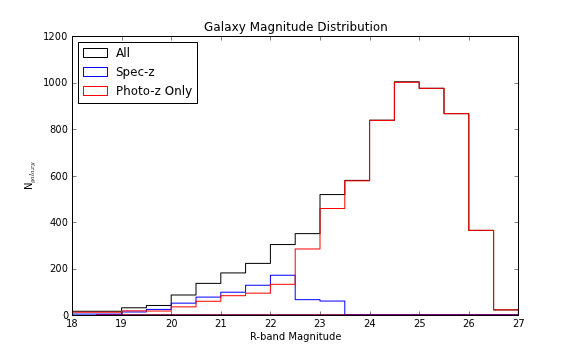
\includegraphics[width=5in]{Chapter4/AnalysisFiles/magdist.png}
	\caption[Musket Ball Cluster spectroscopic and photometric magnitude distribution.]{
	The Musket Ball Cluster spectroscopic (blue) and photometric (red) galaxy magnitude distribution in the $\sim$15'$\times$15' spectroscopic survey area.
	While the DLS photometric survey is complete to $R\sim26$ photometric redshifts are only reliable to $R\sim24$.
		}
	\label{figure:PhotozSpeczMagDist}
\end{figure}

In addition to the deep photometric data we have carried out an extensive spectroscopic survey of the Musket Ball Cluster (see \S\ref{section:MusketBallSpectroscopy} and \S\ref{sec_MBCzcat}).
We have obtained a sample of 738 spectroscopically confirmed galaxy redshifts within an $\sim 18\arcmin \times 18\arcmin$ area centered on the Musket Ball Cluster ($139.05\deg$, $+29.85\deg$).
This survey covers a significant fraction of the galaxies in the area brighter than $R=23$, see Figure \ref{figure:PhotozSpeczMagDist}.
This spectroscopic sample has also provided important information of the accuracy of the photometric redshifts, see Figure \ref{figure:photzVSspecz}, in particular their accuracy of determining cluster galaxy membership.

\begin{figure}
\centering
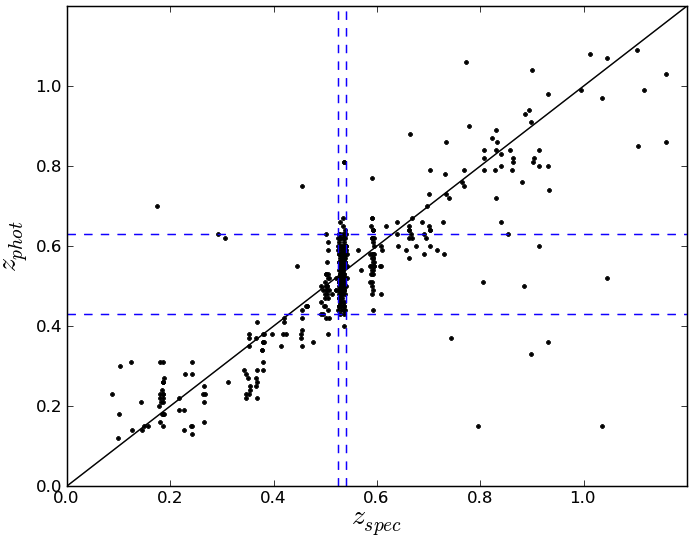
\includegraphics[width=5in]{Chapter4/photVSspec.png}
\caption[Spectroscopic verses photometric redshift for the Musket Ball Cluster.]{
Spectroscopic redshifts verses photometric redshift estimates for the galaxies observed in the Musket Ball Cluster $R<$23.5 magnitude limited survey (discussed in Chapter \ref{chapter:2} and \S\ref{sec_MBCzcat}).
The horizontal dashed blue lines highlight the 0.43$\leq z_{\rm phot} \leq$0.63 range.
63\% of the surveyed galaxies within this range are cluster members.
The verticle dashed blue lines highlight the 0.525$\leq z_{\rm spec} \leq$0.54 or three times the cluster velocity dispersion.
}
\label{figure:photzVSspecz}
\end{figure}


\subsubsection{Fully Probabilistic Membership Determination}

The first of two membership determination methods applied to the Musket Ball Cluster is rooted in the desire to treat both spectroscopic and photometric redshift samples in a consistent manner. 
This method slightly favors minimizing the Poisson noise while still trying to address the systematic contamination error. 
The basic approach is to assign weight to each galaxy roughly based on its probability of being a cluster member.
This weight is defined as the inner product of the redshift probability density function (PDF) of a galaxy $p(z)_i$ and the redshift velocity dispersion of the cluster (assumed to be Gaussian),
\begin{equation}
w_i = \int_{0}^{\infty} p(z)_i \frac{1}{\sigma_{\rm vdisp}\sqrt{2\pi}}e^{\frac{-(z-z_{\rm cluster})^2}{2\sigma_{\rm vdisp}^2}}\mathrm{d}z,
\label{equation:genericz_weight}
\end{equation}
where $\sigma_{\rm vdisp}$ is the redshift velocity dispersion of a cluster a redshift $z_{\rm cluster}$.
Since the redshift uncertainty of a spectroscopically observed galaxy with $z_{\rm spec_{i}}$ is $\ll \sigma_{\rm vdisp}$ and its redshift PDF can be treated as a delta function and Equation \ref{equation:genericz_weight} reduces to
\begin{equation}
w_i = \frac{1}{\sigma_{\rm vdisp}\sqrt{2\pi}}e^{\frac{-(z_{\rm spec_{i}}-z_{\rm cluster})^2}{2\sigma_{\rm vdisp}^2}}.
\end{equation}\label{equation:specz_weight}
Under the assumption of Gaussian photometric redshift errors ($\sigma_{\rm z-phot_{i}} \approx \bar{\sigma}(1+z_{\rm phot_{i}})$; $\bar{\sigma}$=0.07 for the Musket Ball Cluster) Equation \ref{equation:genericz_weight} takes the form
\begin{equation}
w(draw)_i = \int_{0}^{\infty} \frac{1}{\sigma_{\rm z-phot_{i}}\sqrt{2\pi}}e^{\frac{-(z-z_{\rm phot_{i}})^2}{2\sigma_{\rm z-phot_{i}}^2}} \frac{1}{\sigma_{\rm vdisp}\sqrt{2\pi}}e^{\frac{-(z-z_{\rm cluster})^2}{2\sigma_{\rm vdisp}^2}}\mathrm{d}z.
\label{equation:photoz_weight}
\end{equation}

When estimating the galaxy centroid these weights are simply used in conjunction with Equation \ref{equation:WeightedCentroid}.
The bootstrap realizations used in the centroid uncertainty estimate are handled in a slightly different but equivalent manner.
Using these weights we form a cumulative normalized weight distribution for all the galaxies with $R<24$ and within a 9' by 9' region surrounding the Musket Ball Cluster (see Figure \ref{figure:NormWeightDist}).
During the bootstrap sampling process a random number between 0 and 1 is drawn from a uniform distribution, where this random number intersects the weight distribution determines the randomly selected galaxy.
Beyond this weighted draw with replacement the bootstrap uncertainty analysis is standard in all regards.

\begin{figure}
\centering
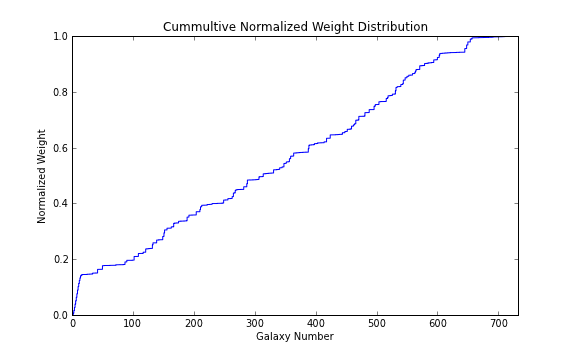
\includegraphics[width=4.5in]{Chapter4/AnalysisFiles/cumnormwghtdist.png}
\caption[Probabilistic scheme; cumulative normalized weight distribution for galaxies being in the Musket Ball Cluster.]{
The resulting cumulative weight distribution for all the galaxies with $R<24$ and within a 9' by 9' region surrounding the Musket Ball Cluster.
This distribution is used to perform a weighted random draw of cluster galaxies (e.g. the green distribution of Figure \ref{figure:ProbWeightDist}) for the galaxy centroid bootstrap analysis.
This distribution is determined by Equations \ref{equation:specz_weight} and \ref{equation:photoz_weight}.
During the bootstrap sampling process a random number between 0 and 1 is drawn from a uniform distribution, where this random number intersects the weight distribution determines the randomly selected galaxy.
Note that the catalog is sorted such that the spectroscopic members are first, thus the noticeably steeper slope for the early galaxy numbers.
}
\label{figure:NormWeightDist}
\end{figure}

Comparing the galaxy redshift distribution of a random bootstrap realization with the redshift distribution of the parent population (Figure \ref{figure:ProbWeightDist}) it is apparent that the fully probabilistic membership determination scheme still includes a large number of galaxies with photometric redshift estimates well outside the cluster redshift velocity dispersion ($z_{\rm cluster}\pm\sigma_{\rm vdisp} \approx 0.53\pm0.004$).
The reason for this is simply that the photometric redshift uncertainties are so large compared to all other pertinent redshift scales.
Thus, galaxies that have the exact same photometric redshift as the cluster are not weighted dramatically more than galaxies with photometric redshift estimates well in front of or behind the cluster.
Take for example two photometric redshift galaxies, one at the cluster redshift ($z=0.53$) and one well behind the cluster at $z_{\phot}=0.79$.
According to Equation \ref{equation:photoz_weight} the galaxy with $z_{\phot}=0.53$ will have a weight of 3.7 while the galaxy with $z_{\phot}=0.79$ will have a weight of 0.37.
Since even in this small projected region around the Musket Ball Cluster the number of fore/background galaxies outnumbers the cluster member, this probabilistic weighting scheme will always result in a significant amount of contamination.
This is likely why \citet{George:2011kv} base their probability of cluster membership both on the expected distribution of the cluster members as well as the field.
Such a method is worth considering for future work but is currently beyond the scope of this dissertation.
Instead we will use an empirical based method to determine our weighting scheme of cluster membership. 


\begin{figure}
\centering
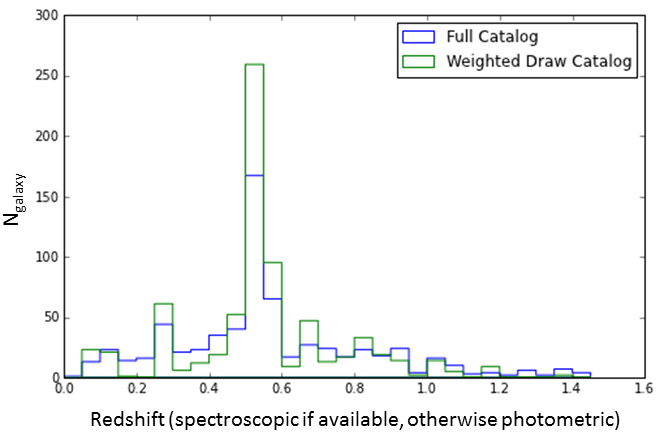
\includegraphics[width=5in]{Chapter4/AnalysisFiles/zdist_randomweightdraw_reformat.png}
\caption[Comparison of parent galaxy redshift distribution with weighted random draw distribution.]{
The redshift (spectroscopic if available, otherwise photometric) distribution of all the galaxies in a 9'$\times$9' area surrounding the Musket Ball Cluster with $R<$24 (blue); and a single bootstrap sample (green) drawn from the fully probabilistic weighted distribution (Figure \ref{figure:NormWeightDist}).
While the probabilistic scheme does work to increase the number of galaxies selected at the cluster redshift ($z=0.53$) it still selects a disproportionate number of galaxies with photometric redshifts outside of the cluster redshift; see that in Figure \ref{figure:photzVSspecz} only 1 galaxy of our spectroscopic survey sample with $z_{\rm phot}$>0.7 is actually at the cluster redshift and only 1 galaxy with $z_{\rm phot}<$0.43 is at the cluster redshift.
}
\label{figure:ProbWeightDist}
\end{figure}


\subsubsection{Empirically Based Membership Determination}

The second method of membership determiniation

Hard redshift cut... why? 1) we are more concerned with purity 

Spectroscopic galaxies should not really be penalized 


spec-z bounds, and justification

photo-z bounds, and justification

photo-z normalization

Photo-z Penalization Factor

This penalization factor is based in the fact that from our magnitude limited survey\footnote{The survey was magnitude limited in regards to the fact that we targeted any galaxy with $R$<23.5, if galaxies had a 0.43$\leq z_{\rm phot} \leq$0.63 there likelihood of being target was twice that of other galaxies. This should not bias the conclusions of this section since we are limiting ourselves to considering just the range 0.43$\leq z_{\rm phot} \leq$0.63. Figure \ref{figure:PhotozSpeczMagDist} shows the approximate completeness of this survey.} (R<23.5) of the Musket Ball we targeted 355 galaxies between 0.43= 3) and 210 of these spectra were between 0.525<specz<0.54 (with quality>=3), see for example the figure below. This translates to a sample purity of 63\%.  Thus I will multiply all of the photo-z galaxy weights by a penalization factor of 0.63.




\begin{figure}
\centering
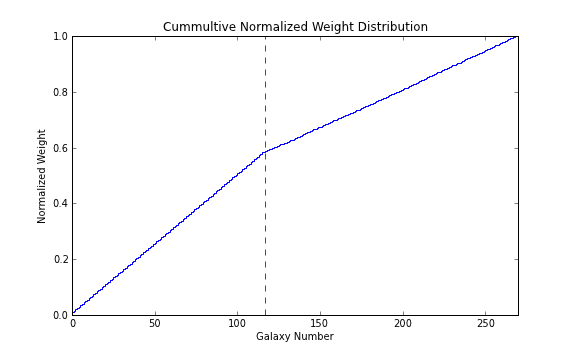
\includegraphics[width=5in]{Chapter4/AnalysisFiles/cumnormwghtdist_zclip_photozpenalty.png}
\caption[Photometric redshift penalization scheme; cumulative normalized weight distribution for galaxies being in the Musket Ball Cluster.]{
The photometric redshift penalization scheme cumulative normalized weight distribution (blue step curve) for galaxies being in the Musket Ball Cluster. 
Galaxies that are spectroscopically confirmed cluster members (0.525$\leq z_{\rm spec} \leq$0.54) are given a weight of 1 and are left of the dashed red line in this sorted sample.
Galaxies that are from the photometric redshift only sample and are within the range 0.43$\leq z_{\rm phot} \leq$0.63 are given a weight of 0.63 and fall to the right of the red dashed line.
Similar, but an alternative, to Figure \ref{figure:NormWeightDist} this distribution is used to perform a weighted random draw of cluster galaxies for the galaxy centroid bootstrap analysis.
}
\label{figure:NormPenaltyWeightDist}
\end{figure}


%\begin{figure}
%\centering
%\includegraphics[width=5in]{ }
%\caption[]{
%}
%\label{}
%\end{figure}

\subsection{Galaxy Location Results}

Perhaps include a table with the actual coordinates and confidence limit values.

Note that we have disregarded the noise caused by subcluster to subcluster contamination. One could consider something like the Walker et al. method (see two component dwarf galaxy).

\begin{figure}
\centering
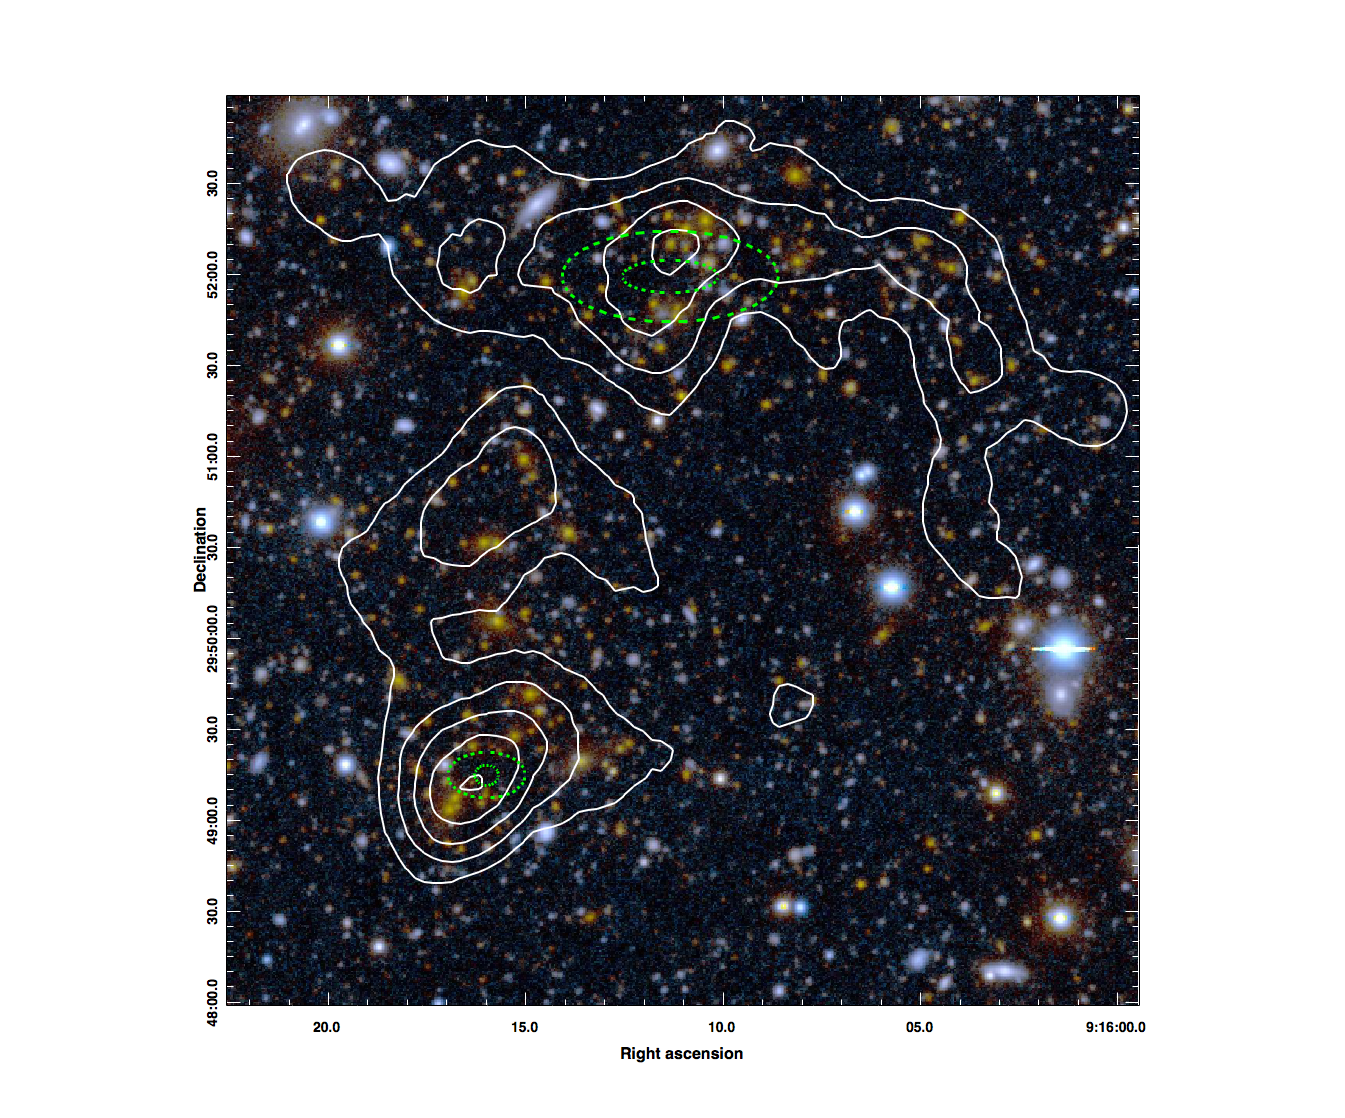
\includegraphics[width=5in]{Chapter4/DLScolor_wGalDenCon.png}
\caption[Musket Ball Cluster galaxy number density map including spectroscopic redshift information.]{
DLS composite $BVR$ color image of the Musket Ball Cluster showing  the galaxies of the two subclusters (predominately orange). 
This figure is similar to Figure \ref{fig2}, however the white contours representing the number density of galaxies now include both spectroscopic and photometric redshift information.
All (117) with galaxies spectroscopic redshift within three times the velocity dispersion of each subcluster were given a weight of 1.
All (270) galaxies without a spectroscopic redshift but with $z_{\rm phot}=0.53\pm0.1$ (the cluster redshift $\pm\sigma_{z_{\rm phot}}$) were given a weight of 0.63.
The photometric redshift sample weight is based on the empirically determined cluster membership purity of this sample, as determined from our magnitude limited spectroscopic survey of the cluster.
The contours begin at $\sim$200 galaxies\,Mpc$^{-2}$ with increments of $\sim$50 galaxies\,Mpc$^{-2}$.
The dashed green ellipses show the approximate galaxy centroid 68\% and 95\% confidence limits for each subcluster.
}
\label{figure:GalDenMap_withspec}
\end{figure}


%--------------------------------------------------------
%--------------------------------------------------------
%--------------------------------------------------------
\section{Gas Location}\label{section:GasLocation}

When estimating the central gas centroid (black circles of Figure \ref{figure:XrayCentroid}), all detected point sources (small green circles with red dashes of Figure \ref{figure:XrayCentroid}) are excluded.
Additionally the diffuse southern gas concentration is excluded (large green rectangular box of Figure \ref{figure:XrayCentroid}).
The remaining X-ray photons in the green semicircle are then used to estimate the gas centroid of the central concentration, using  the \textit{dmstat} function of the Chandra Interactive Analysis of Observations (CIAO) software package.
We note that adaptive smoothing can introduce some artifacts to the image, however we find excellent agreement between the centroid of the smoothed image (black `x' in Figure \ref{figure:XrayCentroid}) and the centroid of the unsmoothed image (black circles of Figure \ref{figure:XrayCentroid}) suggesting that the smoothed map provides a reasonable representation of the gas.

We find that the central gas concentration centroid ($09\fh16\fm13\fs\pm8\fs, 29\fdg50\farcm55\farcs\pm9\farcs$) is offset $5.0\farcs$ from the peak of the gas distribution ($09\fh16\fm15\fs\pm5.5\fs, 29\fdg50\farcm59\farcs\pm5.0\farcs$).
Both are significantly offset between the northern and southern galaxy and WL concentrations.

\begin{figure}
\centering
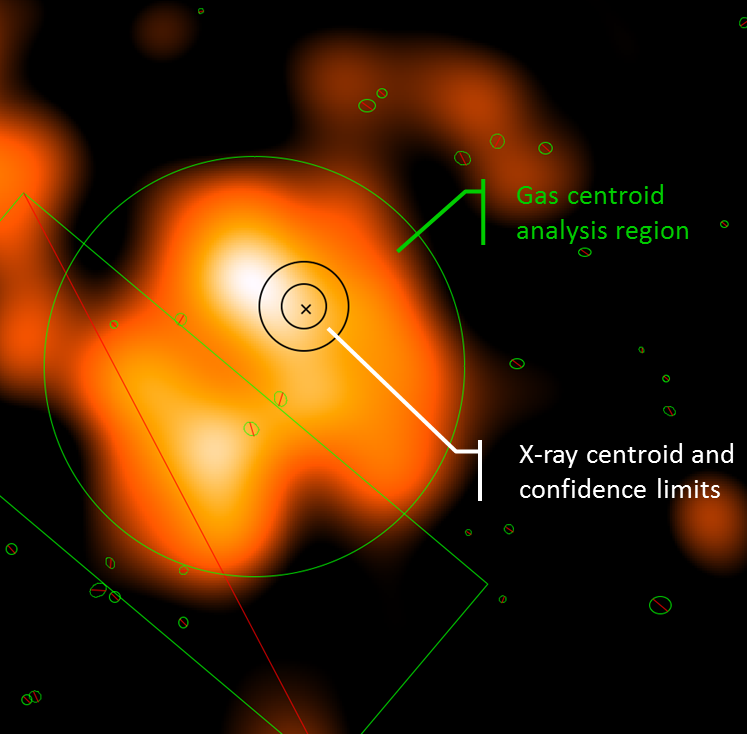
\includegraphics[width=5in]{Chapter4/XrayCentRegions_reformat.png}
\caption[Musket Ball Cluster X-ray map with estimated centroid.]{
Chandra ACIS-I 40\,ks adaptively smoothed X-ray image of DLSCL J0916.2+2951 (the same as Figure \ref{figure:MusketBallXray}).
The green circles and boxes are the SAOImageDS9 inclusion and exclusion regions used in conjunction with the Chandra Interactive Analysis of Observations (CIAO) software package.
The unsmoothed central gas centroid 68\% and 95\% confidence intervals are represented by the black circles.
The smoothed central gas centroid is represented by the black `x'.
The image field-of-view is the same as Figure \ref{fig1}.
}
\label{figure:XrayCentroid}
\end{figure}

%-------------------------------------------------------
%-------------------------------------------------------
%-------------------------------------------------------

\section{Weak Lensing Location}\label{section:WLLocation}

Compare different analysis methods (e.g. james maximum entropy method and my tomography method)

to some degree WL faces the same challenge as the galaxy location in that it is necessary to determine to position of galaxies along the line-of-sight.
however WL is not quite as sensitive due to the broad WL kernel.
(Much of this discuss is unecessary here and the Chapter 2 WL tomography dicussion can be reference)
Might be worth referencing the work of Dietrich et al.

However the breadth of this WL kernel is also a hinderance when determining the WL centroid since line of sight massive structures can induce additional noise in WL centroid estimate of the DM halo centroid.

\subsubsection{Noise and Systematic effects}

\textit{Copied from Chandra/HST proposal. Need to edit.}

Several sources of noise and systematic effect could cause such an offset:
(1) the mass of the northern subcluster pulling off the overall mass
centroid; (2) the gas mass just to the north doing the same; and (3)
unrelated structures along the line of sight. We show below that (2)
is the primary concern and can be solved with Chandra data, and that
(4) HST data are required to tighten up the statistical uncertainty on
the size of offset.  Together, these data will enable measurement of
$\sigma_{\rm DM}m_{\rm DM}^{-1}$.

\textbf{(1)} We model the surface mass density of the north and south subclusters with three NFW halos using masses determined by \citet{Dawson:2012dl}. We recursively estimate the centroid of this model and find an offset $3.4''$ from the true centroid towards the northern subcluster. 
\textbf{(2)} We then combine estimated surface mass densities of the
Central and South gas concentrations with the previous DM surface
densities from step (1) which results in a $7.6''$ centroid offset (dashed red curve of Figure \ref{fig3}).  
For perspective, if we double the gas mass the total offset increases to $10''$, or if we account for the uncertainty in our distribution of the gas mass the modeled centroid offset ranges from $3.4''$ to $9.4''$ (light red region of Figure \ref{fig3}). 
With the proposed Chandra observations we can better constrain the gas mass by approximately a factor of 10 and constrain the distribution of the gas mass so that the resulting uncertainty in the modeled centroid offset is reduced by at least a factor of 2 (dark red region of Figure \ref{fig3}).
\textbf{(3)} As discussed in \citet{Dawson:2012dl} we find no evidence of significant line of sight structures using our full sample of 654 spectroscopic redshifts (with uniform selection over $0<z<1.0$) as well as photometric redshifts. 
Based our findings we confidently rule out any line of sight structures with $M_{\rm 200}\gtrsim1\times10^{12} M_\odot$; any undetected structure will have negligible impact on the offset.
\textbf{(4)} We estimate the noise of the galaxy density and weak lensing centroids by performing the recursive centroid analysis on bootstrap samples of each.
For the galaxy density centroid errors we take 1000 bootstrap samples of the spectroscopically confirmed cluster galaxies and remaining galaxies with $0.43<z_{\rm phot}<0.63$ (roughly the cluster redshift $\pm\sigma_{z_{\rm phot}}$).
Similarly we estimate the weak lensing centroid errors by analyzing 1000 bootstrap samples of the lensed background galaxies.

\section{Gas--Weak Lensing Offset}\label{section:GasWLOffset}

%copied from \citep{Dawson:2012dl}
The peak of the gas distribution ($09\fh16\fm15\fs\pm5.5\fs, 29\fdg50\farcm59\farcs\pm5.0\farcs$) derived from X-rays is offset $1.4\arcmin\pm0.49$ from the North HST WL mass peak ($09\fh16\fm10\fs\pm30\fs, 29\fdg52\farcm10\farcs\pm30\farcs$), and $1.4\arcmin\pm0.14$ from the South HST WL mass peak ($09\fh16\fm15\fs\pm8.0\fs, 29\fdg49\farcm34\farcs\pm6.9\farcs$), and is located near a local minimum in the mass (see Figure \ref{fig3}).
Given the significant offset between the WL and gas locations we are able to use the first method of \citet{Markevitch:2004dl} and place a rough limit on the DM self-interaction cross-section, $\sigma_{\rm DM}$.
This method compares the scattering depth of the dark matter, $\tau_{\rm DM}=\sigma_{\rm DM}m^{-1}_{\rm DM} \Sigma_{\rm DM}$, with that of the ICM gas, $\tau_{\rm ICM}\approx 1$, where $m_{\rm DM}$ is the DM particle mass and $\Sigma_{\rm DM}$ is the surface mass density of the DM particles.
$\Sigma_{\rm DM}$ is approximately the WL measured surface mass density, $\Sigma$, since $\sim80\%$ of a typical cluster's mass is DM \citep{Diaferio:2008js}.
For ease of comparison with the results of \citet{Markevitch:2004dl} and \citet{Merten:2011gu} we examine the surface density averaged over the face of the subcluster within $r$=125\,kpc, which is $\Sigma\approx0.15$\,g\,cm$^{-2}$; thus we find $\sigma_{\rm DM} m_{\rm DM}^{-1} \lesssim 7$\,cm$^2$\,g$^{-1}$.  
Note that we cannot apply the velocity-dependent $\sigma_{\rm DM}$ constraint methods outlined by \citet{Markevitch:2004dl} since our analytic model assumes $\sigma_{\rm DM}$\,=\,0 \citep{Dawson:2012dl, Dawson:2012ub}.


\begin{figure}
\centering
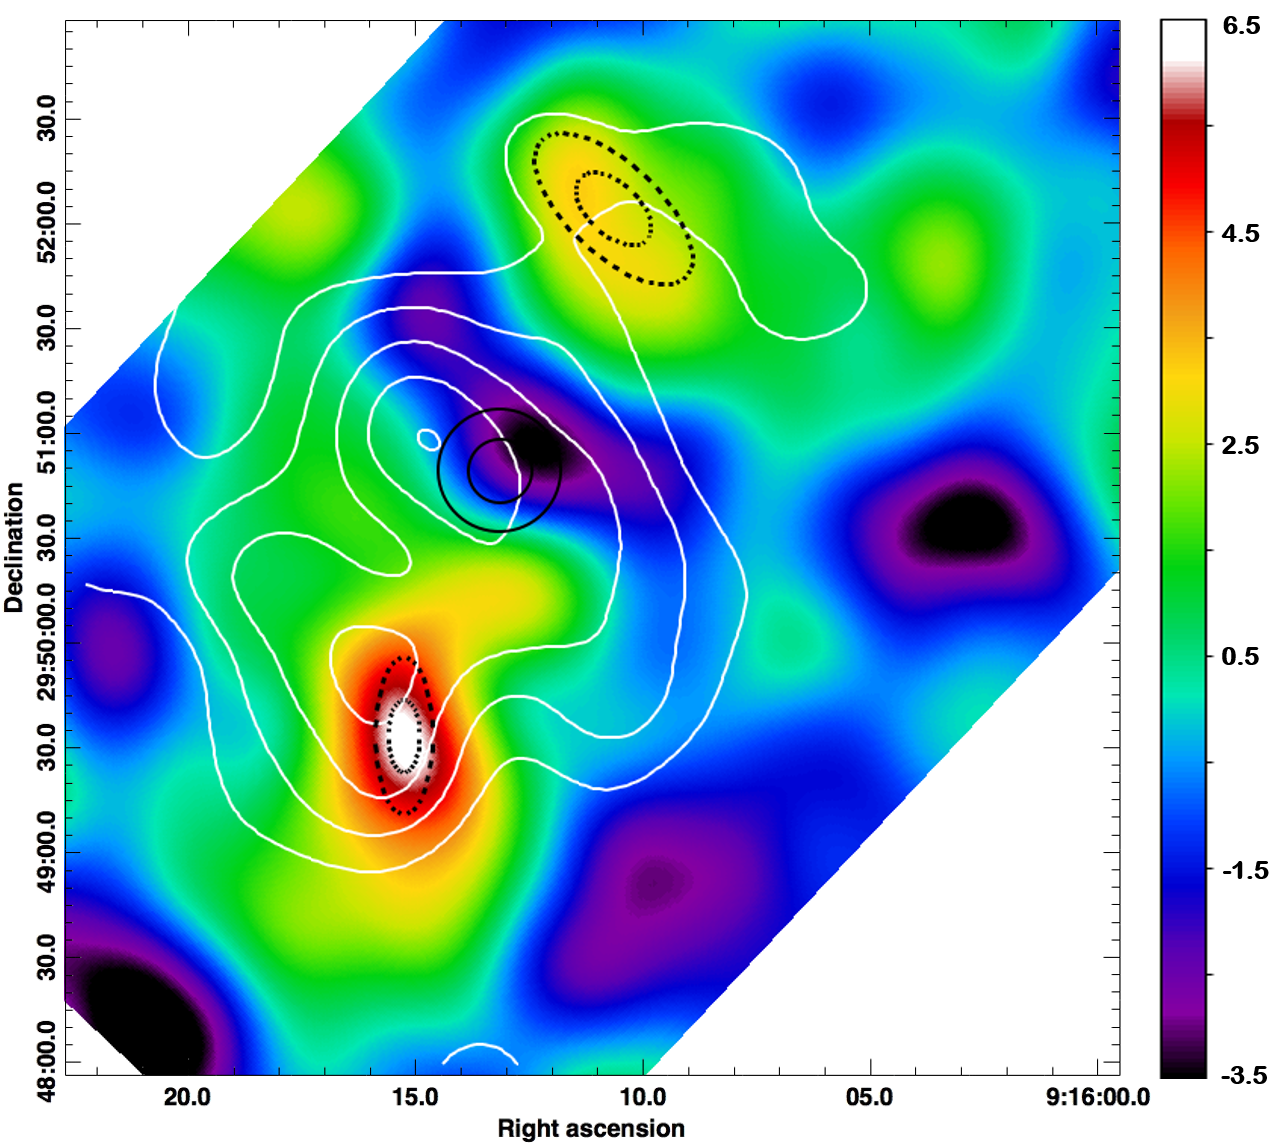
\includegraphics[width=5in]{Chapter4/LensingXrayOverlay.png}
\caption[Musket Ball Cluster weak lensing signal-to-noise map with X-ray map overlay, including centroid locations.]{
HST space-based WL mass signal-to-noise map of the Musket Ball Cluster with the X-ray distribution overlay (white contours).
The 68\% and 95\% centroid confidence intervals are shown for the north and south subcluster WL centroids (dashed black ellipses) as well as the central gas distribution (solid black ellipses).
The majority of the cluster gas is centered $\sim1.4\arcmin$ between the North and South subclusters.
}
\label{figure:LensingXrayOverlay}
\end{figure}


\section{Galaxy--Weak Lensing Offset}\label{section:GalaxyWLOffset}

The offset is now 20.5''

Section text

\begin{figure}
\centering
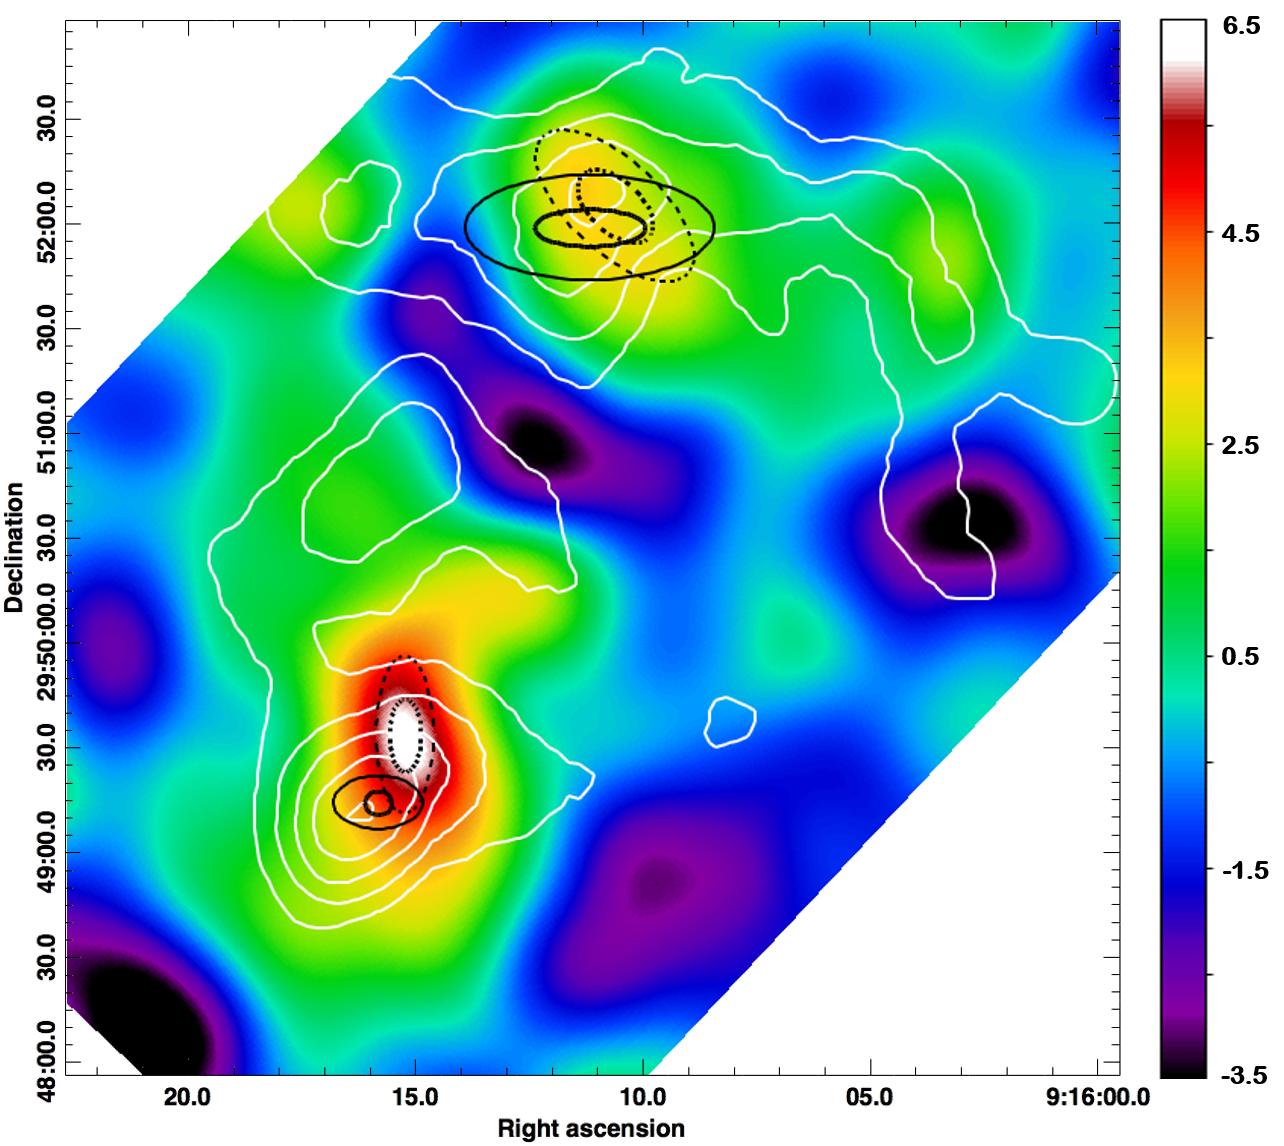
\includegraphics[width=5in]{Chapter4/LensingGalaxyOverlay.png}
\caption[Musket Ball Cluster weak lensing signal-to-noise map with galaxy number density map overlay, including centroid locations.]{
HST space-based WL mass signal-to-noise map of the Musket Ball Cluster with the spectroscopic and photometric redshift based galaxy number density overlay (white contours).
The 68\% and 95\% centroid confidence intervals are shown for the north and south subcluster WL centroids (dashed black ellipses) as well as north and south galaxy number density centroids (solid black ellipses).
Note the 20.5'' offset between the galaxies and the WL mass in the South subcluster.
}
\label{figure:LensingGalaxyOverlay}
\end{figure}



\begin{figure}
\centering
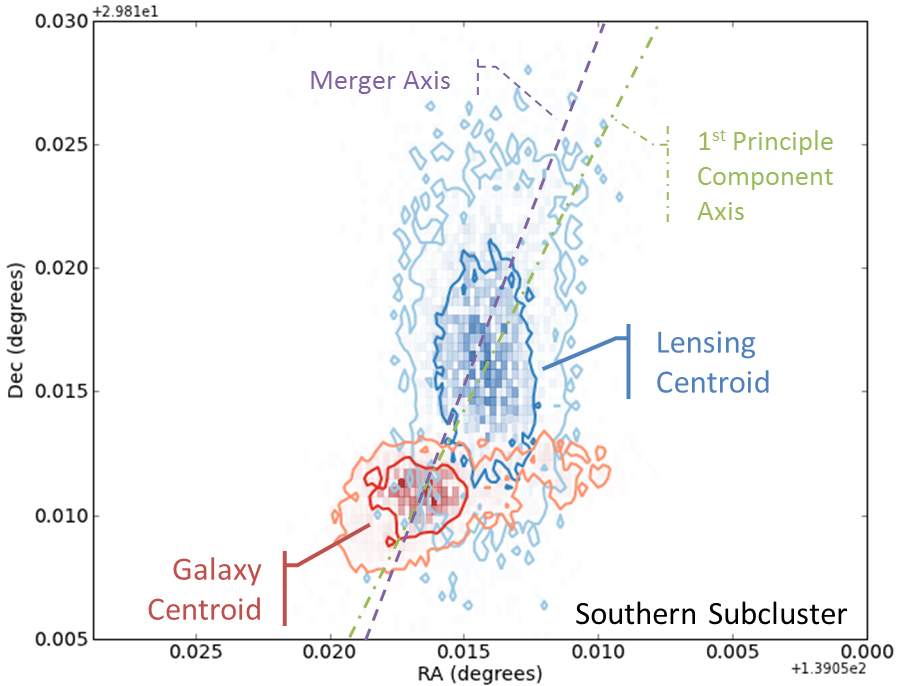
\includegraphics[width=5in]{Chapter4/AnalysisFiles/southcentroids_histplot2d_reformat.png}
\caption[Musket Ball southern subcluster galaxy and weak lensing centroid spatial distribution.]{
Musket Ball southern subcluster WL (blue) and galaxy number density (red) centroid probability density distribution functions constructed from 10,000 respective bootstrap realizations.
The 68\% (dark contours) and 95\% (light contours) confidence intervals are shown for each.
The region shown is 1.5' by 1.5' ($567\times 567\,kpc^2$ at $z$=0.53).
The first principle component axis of two distributions (dot-dashed green line) has a position angle of 159 degrees, this close to the 153 degree position angle of the merger axis of the cluster (dashed purple line; as inferred from a line intersecting the two galaxy centroids) .
}
\label{figure:CentroidDist_South}
\end{figure}

Both centroids in the northern subcluster are less well defined than the centroids in the southern subcluster.
This is likely due to the northern subcluster being approximately half as massive as the northern subcluster.


\begin{figure}
\centering
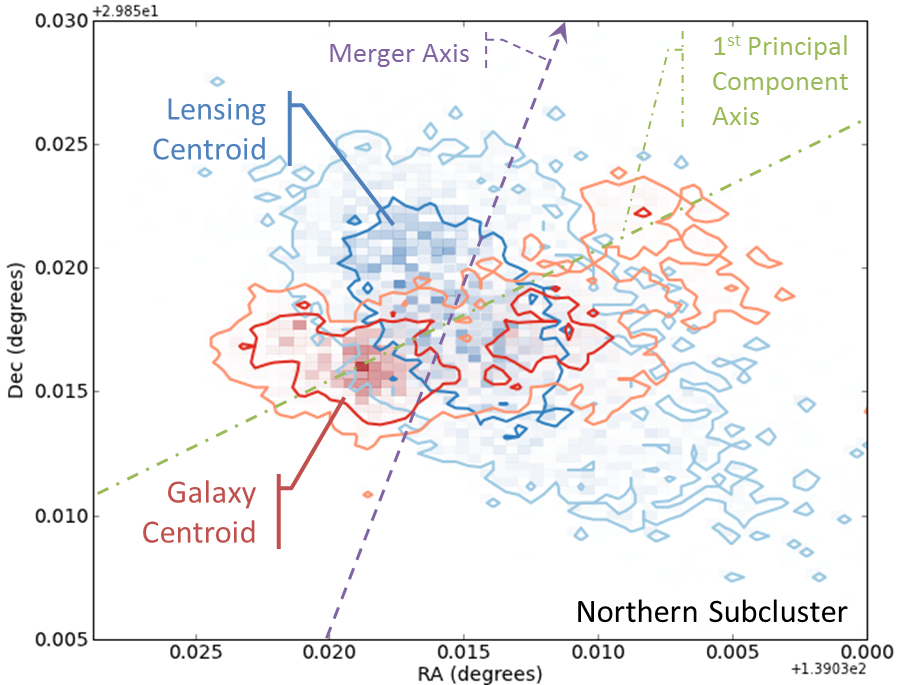
\includegraphics[width=5in]{Chapter4/AnalysisFiles/northcentroids_histplot2d_reformat.png}
\caption[Musket Ball northern subcluster galaxy and weak lensing centroid spatial distribution.]{
Musket Ball northern subcluster WL (blue) and galaxy number density (red) centroid probability density distribution functions constructed from 10,000 respective bootstrap realizations.
The 68\% (dark contours) and 95\% (light contours) confidence intervals are shown for each.
The region shown is 1.5' by 1.5' ($567\times 567\,kpc^2$ at $z$=0.53), the same scale as Figure \ref{figure:CentroidDist_South}.
The merger axis of the cluster (as inferred from a line intersecting the two galaxy centroids) is plotted as a dashed purple line.
Unlike the southern subcluster (Figure \ref{figure:CentroidDist_South}) there does not appear to be a significant offset between between the locations.
Both centroids in the northern subcluster are less well defined than the centroids in the southern subcluster; most notably the galaxy density centroid which appears bimodal.
}
\label{figure:CentroidDist_North}
\end{figure}

Perhaps include some figures discussing systematic offset tests.

The statistical question we pose is:
If the WL and galaxy parent distributions coincide how often would one expect the observed offset of the galaxies leading the WL along the mergers axis\footnote{This is a one-tailed test}.
Assuming the two centroids are expected to coincide in the CDM scenario then the complement of the previous probability is the confidence that $\sigma_{\rm DM}>0$.
Also assuming no systematic errors or random noise not captured by the bootstrap analysis.

\begin{figure}
\centering
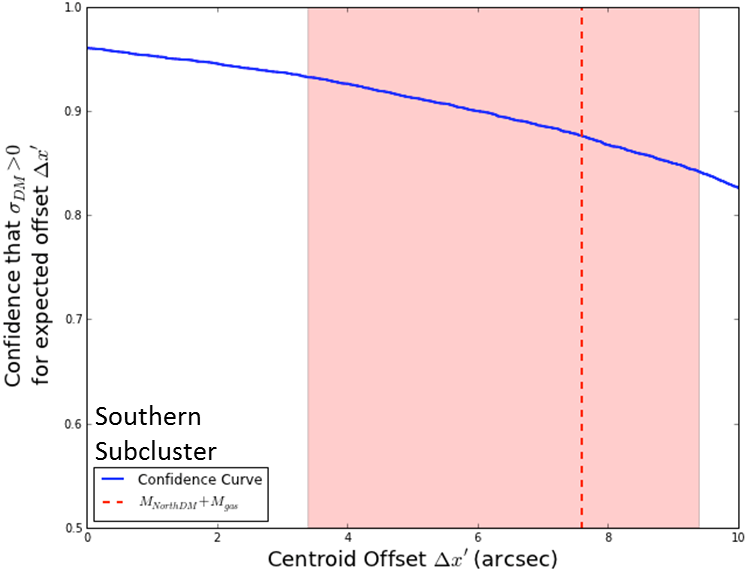
\includegraphics[width=5in]{Chapter4/AnalysisFiles/GalDenVsHSTWL_pzpen_delxPC_south_reformat.png}
\caption[Musket Ball southern subcluster galaxy and weak lensing centroid offset significance.]{

The galaxy-WL centroid offset is measured along the merger axis direction ($x'$) with positive offsets being when the galaxies lead the DM (as expected in the case of SIDM).
}
\label{figure:CentroidSignificance_South}
\end{figure}

\begin{figure}
\centering
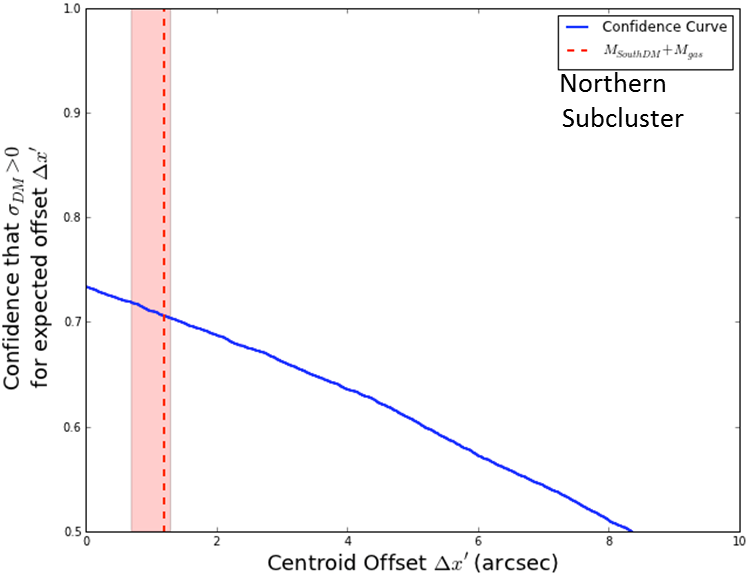
\includegraphics[width=5in]{Chapter4/AnalysisFiles/GalDenVsHSTWL_pzpen_delxPC_north_mergeraxis_reformat.png}
\caption[Musket Ball northern subcluster galaxy and weak lensing centroid offset significance.]{
}
\label{figure:CentroidSignificance_North}
\end{figure}

\section{Discussion}

Discussion text

simulations to study the directional bias of galaxy centroid and WL centroid measurements in dissociative mergers


note importance of fitting both subcluster simultaneously

better modeling of the gas mass and its effect on the systematic centroid offset

note alternatives to centroid estimation, both in measuring the galaxy-dark matter offset as well as just other ways to measure the galaxy centroid, e.g. \citep{Randall:2008hs}

note other means of estimating the offset independent of centroid measurements

For galaxy centroid consider other measurements of the galaxy population location, other than number density, for example weighting the galaxies by luminosity or stellar mass.

Discuss work of \citep{Kahlhoefer:2013wp}

One thing that hasn't been discussed is the typical intrinsic scatter in the lensing centroid. Reference the George, M. work noting that they find that the galaxy center is often $\sim$50kpc from the lensing center. There are a number of problems with directly translating this result to the work discussed here. Since they were dealing with groups of galaxies (typically $\sim$1 order of magnitude less massive and $\sim$1 order of magnitude fewer galaxies than galaxy cluster) they 1) have fewer galaxies with which to beat down the Poisson noise of the centroid estimate, 2) their result is based on which center maximizes the lensing signal of 129 galaxy groups. 

importance of using multiple systems (beat down intrinsic scatter in galaxy-DM offset as well as other sources of noise)

importance of simulations, not only for quantifying the cross-section constraints but also for studying systematic effects (e.g. the intrinsic galaxy-DM offset, both in relaxed cluster as well as merging clusters)

tweak the cluster membership criteria in order to simultainously minimize the joint uncertainty due to cluster membership noise and Poisson noise of the centroid estimate.

\section{Conclusions}

Conclusion text

\textbf{acknowledgements:}
Acknowledgment text
%\end{acknowledgements}

%\bibliographystyle{apj}
%\bibliography{Chapter1/chapter1}{}



%% The References
%\bibliographystyle{thesis}
%\begin{singlespacing}
%  \bibliography{Chapter3/chapter3}
%\end{singlespacing}

        
    % %-----------------------------------------------------------------------
    % 
    % %-------------------------------------------------------- NEW CHAPTER --
    %
    % % -- Chapter 5

%    \newchapter{Perspective}{Perspective: Summary \& Discussion}{Perspective: Summary \& Discussion}
\label{chapter:5}

In this chapter we summarize the work presented in this dissertation.  We follow this summary with a discussion of the challenges that must be overcome if merging clusters are to reach their true potential as dark matter probes and discuss potential solutions to these challenges.

\section{Dissertation Summary}

Over the past century our understanding of the universe has undergone dramatic revisions which have culminated in once inconceivably accurate (percent level) measurements of the composition of the universe.
While the general scientific community agrees upon the composition of the universe, the properties of the bulk of this composition (dark matter and dark energy) remain a mystery.
This dissertation has presented our recent efforts to better understand the properties of dark matter (DM).

In Chapter \ref{chapter:1} we provided a brief review of the history of DM (\S\ref{section:DMhistory}), showing that while Fritz Zwicky provided the first evidence of DM in 1933 \citep{Zwicky:1933ub} it wasn't until the work of Vera Rubin and collaborators \citep{Rubin:1970gu} in the 1970's that DM garnered much attention.
Three general candidates for DM originally dominated the debate.
One possibility was that it was simply massive compact objects made up of standard model particles, another was that it was some new particle, and another was that general relativity needed to be modified.
The MACHO experiment \citep{Alcock:2000bw} eventually ruled out the possibility that massive compact objects made up the bulk of DM, and merging galaxy clusters ruled out modified gravity \citep{Clowe:2006hr} thus providing strong evidence for DM being a new particle.
We reviewed the generally accepted cold dark matter (CDM) properties (\S\ref{section:CDMproperties}) but provided motivation for considering that DM might actually interact with itself other than through gravity (SIDM model; \S\ref{section:SIDMmotivation}).
We also reviewed the possible probes of SIDM (\S\ref{section:SIDMprobes}), highlighting  merging galaxy clusters (\S\ref{section:MergingClustersSIDMprobe}) and the four methods of constraining SIDM with observations of merging clusters.

In Chapter \ref{chapter:2} we introduced the the merging galaxy cluster DLSCL J0916.2+2951 (also known as the Musket Ball Cluster) and presented our multi-wavelength studies of the system.
Our photometric and spectroscopic observations show that the system consists of two subclusters separated by a projected distance of 1.0$\pm$0.1\,Mpc and a line-of-sight velocity difference of $v_{\rm los}=670^{+270}_{-330}$\,km\,s$^{-1}$.
Thus the two subclusters are close enough to be physically associated with one another.
Our weak lensing analysis of the north and south subclusters show that they have comparable mass $1.7^{+2.0}_{-0.72}\times10^{14}$\,M$_\sun$  and $3.1^{+1.2}_{-0.79}\times10^{14}$\,M$_\sun$, respectively.
Suggesting that the system is a major merger.
Our Sunyaev-Zel'dovich effect and X-ray observations show that the cluster gas is located between the two subclusters proving that the Musket Ball Cluster is a post merger system where the collisional gas has become dissociated from the effectively collisionless galaxies and DM.
Thus the Musket Ball Cluster is an excellent candidate to constrain the DM self-interaction cross-section ($\sigma_{\rm SIDM}$).

In Chapter \ref{chapter:3} we discussed the importance of understanding the dynamic history of mergers when attempting to use them to constrain the properties of DM.
We developed a new Monte Carlo based method to discern the properties of dissociative mergers and propagate the uncertainty of the measured cluster parameters in an accurate and Bayesian manner.
We verified it against an existing hydrodynamic N-body simulation, and applied it to two known dissociative mergers: 1ES 0657-558 (Bullet Cluster) and the Musket Ball Cluster.
We find that the dynamic properties of the Musket Ball occupy a significantly different volume of merger phase space than the Bullet Cluster.
The Musket Ball Cluster, being $3.4^{+3.8}_{-1.4}$ times further progressed than the Bullet Cluster, could potentially provide tighter constraints on $\sigma_{\rm DM}$ since the offset between galaxies and dark matter should initially increase with time post-merger for  $\sigma_{\rm DM}>0$.

In Chapter \ref{chapter:4} we compared the locations of the galaxies, gas, and DM in the Musket Ball Cluster to provide insight into the properties of DM.
We constrain the central gas distribution's projected centroid to within 9'' (57\,kpc at $z$=0.53), see \S\ref{section:GasLocation}.
Using both the extensive spectroscopic and photometric redshifts we constrain the galaxy centroid of the northern subcluster to within 5.3" (33\,kpc at $z$=0.53) and the galaxy centroid of the southern subcluster to within 3.3" (21\,kpc at $z$=0.53), see \S\ref{section:GalaxyLocation}.
And using our tomographic WL method applied to the HST measured shapes we constrain the projected WL centroid of the northern subcluster to within 13'' (82\,kpc at $z$=0.53) and the WL centroid of the southern subcluster to within 11'' (69\,kpc at $z$=0.53), see \S\ref{section:WLLocation}.
Our measurement of a significant offset of the gas between the DM in each subcluster enabled us to achieve the constraint $\sigma_{\rm DM} m_{\rm DM}^{-1} \lesssim 7$\,cm$^2$\,g$^{-1}$.
Given the dependence on the surface mass density of this method it is not surprising that this constraint is less than that achieved with more massive mergers \citep{Markevitch:2004dl, Bradac:2008gw, Merten:2011gu}.
Finally in this chapter we investigated the galaxy-WL offset, since if DM self-interacts then the effectively collisionless galaxies might be expected to lead the DM post-merger.
While we find that the galaxies appear to be leading the WL centroid in the southern subcluster by $\sim$20.5'' (129\,kpc at $z$=0.53), see \S\ref{section:GalaxyWLOffset}, this only provides $\sim$85\% confidence that $\sigma_{\rm DM}>0$.
Furthermore, when we account for the observation that the galaxy centroid appears to trail the WL centroid in the northern subcluster by $\sim$7.4'' (47\,kpc at $z$=0.53), the confidence that $\sigma_{\rm DM}>0$ falls to $\sim$55\%.
While the SIDM scenario is slightly preferred over the CDM scenario it is not significantly so.
SIDM simulations of the Musket Ball Cluster are needed to turn these observations into quantitative constraints on $\sigma_{\rm DM}$.


\section{Discussion on the Path Forward}

There are a number of outstanding uncertainties/challenges that must be overcome before merging clusters are proven capable of obtaining the necessary SIDM constraints to either measure $\sigma_{\rm DM}$ or constrain it to the point of being astrophysically uninteresting.

\subsection{Intrinsic Scatter in the Location of Galaxies and DM/Lensing}

Perhaps the most notable challenge is related the results from the recent theoretical studies of SIDM effects in merging clusters by \citet{Kahlhoefer:2013wp} (which were presented in the arXiv one week before the completion of this dissertation).
There are a number of promising results from their study which support claims made previously in this dissertation (e.g., they confirm the expectation that the galaxy-DM offset increases following the merger, and also confirm that for some models of DM, common mergers such of the Musket Ball Cluster can have more constraining power than extreme mergers such as the Bullet Cluster)
However, one result from their study casts doubt on the possible effectiveness of merging galaxy clusters to constrain SIDM.
In particular, they find that the typical galaxy-DM offset ranges between $\sim$5--15\,kpc for allowable ranges of $\sigma_{\rm DM}$.
This is much smaller than the galaxy and WL centroid uncertainties typically measured for galaxy clusters ($\sim$20--100\,kpc).
And since most mergers don't occur directly in the plane of the sky, the observable projected offset will be $\lesssim5$--15\,kpc, assuming the \citet{Kahlhoefer:2013wp} results are correct.
Even disregarding intrinsic scatter of the galaxy-DM location and systematic offset effects due to the dissociated gas and other subcluster mass, it will take a large number of dissociative mergers to reach the $\sim$10\,kpc offset level.
Take for example the Musket Ball Cluster studied in this dissertation.
We find that we are able to constrain the galaxy centroid in each subcluster to $\sim\pm$25\,kpc and the WL centroid in each subcluster to $\sim\pm$70\,kpc.
This roughly translates to a centroid offset uncertainty of $\sigma_{\rm offset}\sim$80\,kpc (again for argument's sake disregarding other systematic offset errors).
Since the offset measurement is largely Poisson noise dominated (i.e. $\sigma_{\rm offset}\propto N^{-1/2}$), it will take roughly 14--128 dissociative mergers\footnote{Assuming that two centroid offset measurements can be made for each dissociative merger, since there are two subclusters per dissociative merger.} similar to the Musket Ball Cluster to achieve the necessary centroid accuracy of $\lesssim$5--15\,kpc.
While this example is highly simplified, and it is not clear how general or accurate the \citet{Kahlhoefer:2013wp} results are,  it does highlight the magnitude of this challenge and the importance of investigating it further.

Along these lines, the intrinsic scatter between the location of the galaxies and DM in galaxy clusters is still not accurately known.
If the intrinsic scatter is of order the centroid measurement uncertainty then this will add significantly to the challenge of constraining SIDM with the galaxy-WL offset measurement in dissociative mergers.
Two immediate means of quantifying this intrinsic scatter is through studies of the scatter in existing simulations and observations of relaxed cluster systems.
A number of high resolution simulations of relaxed clusters exist \citep[e.g.][which include both CDM and SIDM simulations]{Peter:2012vi, Rocha:2012tr}.
By treating the subhalos in the cluster simulation as galaxies, one could estimate the intrinsic galaxy-DM offset.
Alternatively a purely observational approach could study the galaxy-lensing offset in a sample of well measured relaxed clusters.
For example the Cluster Lensing and Supernova Survey with Hubble (CLASH) galaxy cluster sample (20 relaxed clusters, $\sim$5--30\,M$_\sun$) provides excellent weak and strong lensing data to locate the DM as well as 16-band photometric redshifts to identify cluster members for the galaxy population location.
Researchers of the Merging Cluster Collaboration are pursuing both avenues.

\subsection{Find and study more dissociative mergers}

Regardless of the magnitudes involved in the intrinsic scatter of the galaxy-WL/DM offset, it will be important to study as many dissociative mergers as possible in order to reduce this noise.
Fortunately the number of confirmed dissociative mergers has been increasing at a rapid rate (see Figure \ref{figure:N_Mergers}).
Prior to 2013 all of the dissociative mergers were serendipitously discovered, often requiring photometric, spectroscopic, lensing and X-ray observations for identification.
The rapid rise in the number of confirmed mergers after 2013 is due to the radio relic selection method.
Radio selection is an efficient way to identify dissociative mergers because the shock produced by a merger results in a ``radio relic'' (uniquely diffuse emission in an arc around part of the cluster, e.g. van Weeren et al. 2010).
So rather than needing photometric, spectroscopic, lensing and X-ray observations it is possible to identify dissociative mergers with just radio observations.
Thus wide-area radio surveys can provide many candidates. 
NVSS has already found a few dozen, and LOFAR is projected to find about 1000 \citep{Nuza:2012fu}.
The Merging Cluster Collaboration has begun an extensive follow-up of these radio relic mergers (see the red points in Figure \ref{figure:N_Mergers} after 2013) with Keck spectroscopy, Subaru and HST imaging, and Chandra and XMM X-ray imaging.

\begin{figure}
\centering
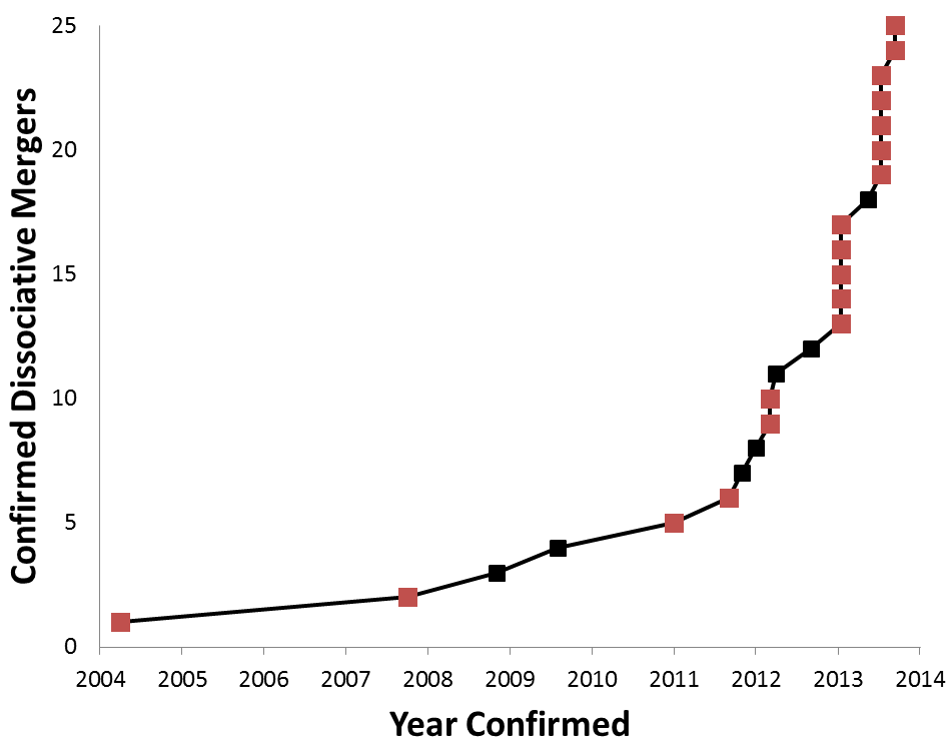
\includegraphics[width=4in]{Chapter5/NumberOfConfirmedDissociativeMergers.png}
\caption[Number of confirmed dissociative mergers as a function of time.]{
Number of confirmed dissociative mergers as a function of time.
The red points identify mergers that the Merging Cluster Collaboration are studying to  constrain the properties SIDM.
Up until 2013 dissociative mergers were all serendipitously discoveries.
The rapid rise in the number of confirmed mergers after 2013 is due to the radio relic selection method.
}
\label{figure:N_Mergers}
\end{figure}

Another promising avenue of dissociative merger discovery is with the optical-Sunyaev Zel'dovich effect identification method that lead to the discovery of the Musket Ball Cluster.
Since the DES optical survey \citep{Collaboration:2005vv} will overlap much of the SPT \citep{Ruhl:2004io} and ACT \citep{Hincks:2010ff} Sunyaev-Zel'dovich effect (SZE) surveys it will be possible to search for significant offset of an SZE peak between a bimodal distribution of galaxies.
Based on the simulated and observed SZE cluster counts in the SPT survey \citep{Vanderlinde:2010hr, Song:2012tz} and the fraction of all clusters that are dissociative mergers \citep{ForeroRomero:2010cc} we estimate that $\sim$50 detectable dissociative mergers will be observed in the 4000 degree$^2$ SPT-DES survey.  Selection bias will result in mergers with large mass (i.e., better signal-to-noise) and large projected separations (i.e., later stage mergers where the expected DM-galaxy offset is maximized).  These will potentially be some of the best dissociative mergers with which to constrain $\sigma_{\rm DM}$.


Looking further into the future, the LSST optical survey \citep{Tyson:2002hn} will cover a larger area than DES and go much deeper.
When it is coupled with upcoming all-sky X-ray surveys (e.g., eROSITA), that will enable much better angular resolution of the gas compared to SPT and ACT, there is the possibility to discover thousands of dissociative mergers.
Additionally, LSST with have multi-band photometric redshifts and excellent lensing quality data.
Thus it is conceivable that the field of dissociative merger science will enter an era where the statistical errors no longer dominate the measurements. 

\subsection{Going from Observations to Dark Matter Constraints}

Beyond the challenges associated with making the galaxy-DM offset measurement there remains the challenge of translating that measurement into a constraint on $\sigma_{\rm DM}$.
This challenge has both an observational element and a theoretical element.

Observationally it is possible to measure the projected galaxy-DM offset but this needs to be translated into a three-dimensional offset.
As noted in Chapter \ref{chapter:3}, there are severe limitations in our ability to do this, largely due to the difficulty in constraining the angle of the merger axis with respect to the plane of the sky ($\alpha$).
With just the commonly available measurements of the subclusters (mass, relative velocities along the line of sight, and projected separation) the magnitude of the three-dimensional distance errors often exceeds the actual distances being measured (see e.g.\,$d_{\rm 3D}$ of Tables \ref{bulletresultparam} and \ref{musketballresultparam}).
This is potentially a serious problem since there is only a factor of $\sim$2--4 difference between the expected galaxy-DM offset of different $\sigma_{\rm DM}$ models \citep{Markevitch:2004dl, Kahlhoefer:2013wp}.
Fortunately though, moderate constraints on $\alpha$ can translate to significant constraints on 
$d_{\rm 3D}$.
Take for example the Bullet Cluster with the added temporal prior (\S\ref{sec_addedprior}) where a factor of two improvement on the $\alpha$ uncertainty was accompanied by a factor of 9 improvement on the $d_{\rm 3D}$ uncertainty.
An added advantage of our radio relic sample is that radio polarization measurements of the radio relic can place an upper limit on $\alpha$ \citep{Ensslin:1998tx}, for example in the case of CIZA J2242.8+5301 the polarization measurements translated to an upper limit on $\alpha$ of 30\,degrees.
Thus it is conceivable that this element of the challenge is not a daunting as it might seem.

The other major element of the challenge of translating the galaxy-DM measurement into a constraint on $\sigma_{\rm DM}$ is theoretically predicting the galaxy-DM offset for a given $\sigma_{\rm DM}$.
\citet{Randall:2008hs} showed that a promising technique is simulating a merger with collisionless ``galaxy'' particles and DM particles with varying $\sigma_{\rm DM}$ between runs.
However there were a number of simplifying assumptions in their simulations that must be addressed if dissociative mergers are going to accurately constrain $\sigma_{\rm DM}$: 

\textit{(i)} They only modeled a single analog of the Bullet Cluster. 
By only choosing to model one analog of the Bullet Cluster, that albeit was representative of the most likely observed subcluster masses and projected separation, they failed to propagate the uncertainty in the observed merger parameters to the uncertainty in the expected offset for a given $\sigma_{\rm DM}$; thus the lack of uncertainty estimates in there expected offset results.

\textit{(ii)} The collision velocity in their simulation is extremely high.
They based their choice of collision velocity on the Mach number of the gas shock feature, but as noted in Chapter \ref{chapter:3} there are physical reasons this velocity is an overestimate of the true relative velocity.
This resulted in an overestimate of the expected offset.
	
\textit{(iii)} The galaxies were uniformly distributed in the DM halo and they used an unreasonably large number of galaxy particles. 
This unrealistic assumption fails to account for the intrinsic scatter related to the Poisson noise associated with the galaxies (see \S\ref{section:GalaxyLocation}).

\textit{(iv)} Galaxies were not embedded in their own DM subhalos.
This could affect the expected offset between the galaxies and the cluster DM halo. The DM subhalos will experience a drag force due to  $\sigma_{\rm DM}$, and this will be translated to some degree into a gravitational drag force on the galaxies due to the gravitational dominance of the subhalos on small scales. 

\textit{(v)} The central densities of the subclusters were unphysically cuspy for the chosen $\sigma_{\rm DM}$.
As \citet{Rocha:2012tr} found the central density of SIDM halos becomes cored as $\sigma_{\rm DM}$ increases.
Since the interaction rate scales roughly as the SIDM density squared, using King profiles for all the halos can result in overestimates of the expected offset. 

At the heart of problems \textit{i}--\textit{iv} is the fact that the simulations failed to take into account the wealth of cosmological prior information.
One possible solution to this and all of the associated problems is identifying likely merger analogs in large cosmological N-body simulations rather than setting up a simplified toy model of the merger.
And then resimulating these analogs at higher resolution with varying $\sigma_{\rm DM}$.
Perhaps the best means of identifying analog mergers is through importance sampling. 
Where the known properties of merger in the cosmological simulation are cast in terms of the observable properties (subcluster masses, relative line-of-sight velocity, and projected separation), then given the PDF's of the observed properties a likelihood of each simulated analog can be calculated.
Because each simulated analog of the observed merger will have an associated likelihood, we could then create a posterior PDF of the expected galaxy-DM offset for a given $\sigma_{\rm DM}$ that marginalizes over all other uncertainties associated with a given merger.
It will then be possible to combine the $\sigma_{\rm DM}$ constraints in a fair and well defined manner from an ensemble of dissociative mergers and reduce the noise associated with the galaxy-DM offset constraint method.

\section{Concluding Remarks}

The work of this dissertation has highlighted the promise that merging galaxy clusters offer to either measure $\sigma_{\rm DM}$ or constrain it to the point of being astrophysically uninteresting.
It has also highlighted the many challenges that must be overcome before this promise can be realized.
This is an exciting time as the merging galaxies cluster science will face most these challenges within the next couple years.
While we many not have any definitive results on SIDM in this time, we will have definitively assessed the value of merging galaxy clusters as probes of SIDM.

%\bibliographystyle{apj}
%\bibliography{Chapter1/chapter1}{}



%% The References
%\bibliographystyle{thesis}
%\begin{singlespacing}
%  \bibliography{Chapter3/chapter3}
%\end{singlespacing}



    % % ----------------------------------------------------------------------
    % 
    %% % -- Appendices
    %
    %\appendix
    %
    %
    %% % ----------------------------------------------------------------------
    %% 
    %% %------------------------------------------------------- NEW APPENDIX --
    %%
    %% % -- Appendix 1
    %
    %
    \appendix
\chapter{Dynamics of Merging Clusters Appendix}
\label{chap:dynamicsappendix}

\section{Potential Energy of Two Truncated NFW Halos}\label{potentialsec}

Generically the potential energy of a two-halo system with center to center separation $r$ is 
\begin{equation}
V(r) = \int \Phi_1(r') dm_2,
\label{potint}
\end{equation}
where $\Phi_1(r')$ is the gravitational potential of halo 1 as a function of radial distance $r'$ from the center of the halo 1 to the mass element of halo 2, $dm_2$.  
I derive $\Phi_1(r)$ for the case of a truncated NFW halo in \S \ref{nfwpotential}.
The integral of equation \ref{potint} can be approximated as a summation over $N \times N$ mass elements, $m_{2_{ij}}$, each with area $dr\times d\theta$, where $i$ and $j$ range from $0 \rightarrow N-1$,
\begin{displaymath}
V(r) \approx \sum_{i=0}^{N-1}\sum_{j=0}^{N-1} \Phi_1(r'_{ij}+\epsilon) m_{2_{ij}},
\end{displaymath}
where $r'_{ij}$ is the distance from the center of halo 1 to the 2$^{\rm nd}$ halo's mass element $m_{2_{ij}}$, as derived in \S\ref{masselements}, and $\epsilon$ is the softening length which reduces the effects of artificial singularities.

\subsection{Truncated NFW Gravitational Potential}\label{nfwpotential}

For an axially symmetric mass distribution the potential can be expressed as a series of Legendre Polynomials

\begin{equation}
\Phi_n(r) = -\frac{2\pi G}{(n+1/2)r^{n+1}} \int_{0}^{r} r'^{n+2} \rho_{n}(r')\,dr' -\frac{2\pi G r^n}{n+1/2} \int_{r}^{\infty} r'^{1-n} \rho_n(r')\,dr' 
\label{axsympot}
\end{equation}
where
\begin{equation}
\rho_n(r) = (n+1/2) \int_{0}^{\pi} \rho(r,\theta) P_n(\cos \theta) \sin \theta \,d\theta.
\label{lengden}
\end{equation}

Assuming a spherical NFW halo
\begin{displaymath}
\rho_{\rm NFW}(r) = \frac{\rho_s}{r/r_s(1+r/r_s)^2}
\end{displaymath}
only the zero$^{\rm th}$ order term of Equation \ref{lengden} remains
\begin{displaymath}
\rho_{\rm NFW}(r) = \rho_0(r)
\end{displaymath}
and Equation \ref{axsympot} reduces to
\begin{eqnarray}
\Phi_{\rm NFW}(r) & = & -\frac{4\pi G}{r}\int_{0}^{r} r'^2 \rho_{\rm NFW}(r')\,dr' - 4\pi G \int_{r}^{\infty}r' \rho_{\rm NFW}(r')\,dr' \nonumber\\
\Phi_{\rm NFW}(r) & = & -\frac{4\pi G \rho_s}{r} \left[ \int_{0}^{r} \frac{r'^2}{r'/r_s(1+r'/r_s)^2}\,dr' + r \int_{r}^{\infty} \frac{r'}{r'/r_s(1+r'/r_s)^2}\,dr' \right]. \nonumber
\end{eqnarray}
Since I truncate the NFW halo at $r_{200}$ the $\infty$ in the second integral becomes $r_{200}$ and
\begin{equation}
	\Phi_{\rm NFW_T}(r)=
	\begin{cases}
 		-\frac{4\pi G}{r} \rho_s r_s^3 \left[ \ln (1+r/r_s)-\frac{r}{r_s+r_{200}} \right], &\text{if $r\leq r_{200}$;}\\
  		-\frac{G M_{200}}{r}, &\text{if $r>r_{200}$.}
  	\end{cases}
\end{equation}

\subsection{Mass Elements of a Truncated NFW Halo}\label{masselements}

Given the differential mass elements for a spherically symmetric halo
\begin{displaymath}
dm = 2\pi\rho(r,\theta) r^2 \sin(\theta) d\theta\,dr,
\end{displaymath}
and discretizing the mass into elements with lengths $\delta r = r_{200_2}/N$ and $\delta\theta = \pi/N$ the halo 2 mass elements are given by
\begin{displaymath}
m_{ij} = 2\pi \int_{i\,\delta r}^{(i+1)\delta r} \int_{j\,\delta\theta}^{(j+1)\delta\theta} \rho(r') r'^2 \sin(\theta') d\theta'\,dr'.
\end{displaymath}
For an NFW halo this becomes
\begin{displaymath}
m_{ij} = 2\pi\rho_s r_s^3 \left[\cos(j\,\delta\theta)-\cos\left((j+1)\delta\theta\right) \right] \left[ \left( 1+\frac{(i+1)\delta r}{r_s}\right)^{-1} - \left(1+\frac{i\,\delta r}{r_s}\right)^{-1} + \ln\left[\frac{(i+1)\delta r+r_s}{i\,\delta r+r_s}\right]\right].
\end{displaymath}

\clearpage

\section{Musket Ball Cluster Redshift Catalog}\label{sec_MBCzcat}

The Musket Ball Cluster redshift catalog (Table \ref{table_MBCzcat}) contains 738 spectroscopically confirmed galaxy redshifts.  The galaxies are within an $\sim 18\arcmin \times 18\arcmin$ area centered on the Musket Ball Cluster ($139.05\deg$, $+29.85\deg$).  The source of the redshifts are from three separate spectroscopic surveys: 1) \emph{LRIS 2007} was carried out on 2007 January 15 using the Keck:I LRIS instrument, 2) \emph{DEIMOS 2011A} was carried out on 2011 March 1 \& 2 using the Keck:II DEIMOS instrument, and 3) \emph{DEIMOS 2012B} was carried out on 2013 January 16 using the Keck:II DEIMOS instrument.

The \emph{DEIMOS 2011A} observations consisted of 6 slit masks  with 1\arcsec slits and using the 1200\,line\,mm$^{-1}$ grating, tilted to a central wavelentgh of 6700\,\AA, resulting in a pixel scale of 0.33\,$\AA$\,pixel$^{-1}$, a resolution of $\sim1.1$\,\AA (50\,km\,s$^{-1}$), and typical wavelength coverage of 5400\AA\,to 8000\AA. 
The \emph{DEIMOS 2013B} observations consisted of 1 slit mask with 1\arcsec slits and using the 1200\,line\,mm$^{-1}$ grating, tilted to a central wavelentgh of 6200\,\AA, resulting in a pixel scale of 0.33\,\AA\,pixel$^{-1}$, a resolution of $\sim1$\,\AA (50\,km\,s$^{-1}$), and typical wavelength coverage of 4900\AA\,to 7500\AA. 
The exposures for each DEIMOS mask ($\sim3\times20$\,minutes) were combined using the DEEP2 version of the spec2d package \citep{Newman:2012ta}.
This package combines the individual exposures of the slit mosaic and performs wavelength calibration, cosmic ray removal and sky subtraction on slit-by-slit basis, generating a processed two-dimensional spectrum for each slit. 
The spec2d pipeline also generates a processed one-dimensional spectrum for each slit.
This extraction creates a one-dimensional spectrum of the target, containing the summed flux at each wavelength in an optimized window. 
Table \ref{table_MBCzcat} only includes high quality (Q $\geq$ 3, see \citet{Newman:2012ta} for an explanation on the quality codes) galaxy spectra.
Details of the \emph{LRIS 2007} observations and reduction are discussed in the Deep Lens Survey data release paper (Wittman et al. in prep).

%% The values (usually only l,r and c) in the last part of
%% \begin{deluxetable}{} command tell LaTeX how many columns
%% there are and how to align them.
\begin{deluxetable}{llcccccc}

%% Keep a portrait orientation

%% Over-ride the default font size
%% Use 8pt
\tabletypesize{\scriptsize}

%% Use \tablewidth{?pt} to over-ride the default table width.
%% If you are unhappy with the default look at the end of the
%% *.log file to see what the default was set at before adjusting
%% this value.
\tablewidth{0pt}

%% This is the title of the table.
\tablecaption{Musket Ball Cluster Redshift Catalog\label{table_MBCzcat}}

%% This command over-rides LaTeX's natural table count
%% and replaces it with this number.  LaTeX will increment
%% all other tables after this table based on this number
%\tablenum{4}

%% The \tablehead gives provides the column headers.  It
%% is currently set up so that the column labels are on the
%% top line and the units surrounded by ()s are in the
%% bottom line.  You may add more header information by writing
%% another line between these lines. For each column that requries
%% extra information be sure to include a \colhead{text} command
%% and remember to end any extra lines with \\ and include the
%% correct number of &s.
\tablehead{\colhead{RA} & \colhead{Dec} & \colhead{PosErr} & \colhead{z} & \colhead{$\sigma$z} & \colhead{Source} & \colhead{R } & \colhead{$\sigma$R} \\
\colhead{(hh:mm:ss.sss)} & \colhead{(dd:mm:ss.ss)} & \colhead{(arcsec)} & \colhead{} & \colhead{} & \colhead{} & \colhead{(mag)} & \colhead{(mag)} }
%% All data must appear between the \startdata and \enddata commands
\startdata
09:15:40.142 & +29:55:06.71 & 0.5 & 0.234777 & 0.000020 & DEIMOS 2011A & 20.983 & 0.007 \\
09:15:41.501 & +29:47:07.64 & 0.5 & 0.530381 & 0.000024 & DEIMOS 2011A & 23.398 & 0.048 \\
09:15:41.682 & +29:55:13.05 & 0.5 & 0.704062 & 0.000033 & DEIMOS 2011A & 22.586 & 0.024 \\
09:15:41.726 & +29:56:12.79 & 0.5 & 0.498200 & 0.000015 & DEIMOS 2011A & 22.664 & 0.016 \\
09:15:42.418 & +29:46:55.71 & 0.5 & 0.899342 & 0.000101 & DEIMOS 2011A & 22.246 & 0.017 \\
\enddata
%% Include any \tablenotetext{key}{text}, \tablerefs{ref list},
%% or \tablecomments{text} between the \enddata and
%% \end{deluxetable} commands

%% General table comment marker
\tablecomments{Table \ref{table_MBCzcat} is published in its entirety in the electronic
edition of the {\it Astrophysical Journal}.  A portion is shown here
for guidance regarding its form and content.}

%% No \tablerefs indicated

\end{deluxetable}

\clearpage

\section{Bullet Cluster Result Plots}\label{sec_bcresults}

This section contains the parameter results array plots for the Bullet Cluster case including the added temporal prior of \S\ref{sec_addedprior}.
For ease of display the parameters are grouped in three categories (\emph{Input}, \emph{Geometry}, and \emph{Velocity \& Time}) resulting in a six subplot results array, see Figure \ref{fig_resultsarray}.
The \emph{Input} parameters consist of: M$_{200_1}$, M$_{200_2}$, $z_1$, $z_2$,	and $d_{\rm proj}$, where halo 1 refers to the ``main'' subcluster and halo 2 refers to the ``bullet'' subcluster.
The \emph{Geometry} parameters consist of the randomly drawn $\alpha$, and calculated $d_{\rm 3D}$, and $d_{\rm max}$.
The calculated \emph{Velocity \& Time} parameters consist of:  $TSC_0$, $TSC_1$, and $T$.

\begin{figure}[b]
\includegraphics{Appendix1/ResultsArray_RevB.png}
\caption{
For ease of display the results array is divided into six subplots, Figures \ref{fig_bc_inin}--\ref{fig_bc_geovt}.
The Input parameters consist of: M$_{200_1}$, M$_{200_2}$, $z_1$, $z_2$,	and $d_{\rm proj}$.
The calculated Geometry parameters consist of: $\alpha$, $d_{\rm 3D}$, and $d_{\rm max}$.
The calculated Velocity \& Time parameters consist of:  $v_{\rm 3D}(t_{\rm obs})$, $v_{\rm 3D}(t_{\rm col})$, $TSC_0$, $TSC_1$, and $T$.
\label{fig_resultsarray}}
\end{figure}
\clearpage

\begin{figure}
\includegraphics{Appendix1/bullet_shockprior_input-input.png}
\caption{Bullet Cluster marginalized \emph{Input vs.\,Input} parameters result plots, for the case including the added temporal prior of \S\ref{sec_addedprior}. Dark and light blue colors correspond to 68\% and 95\% confidence intervals, respectively.  The black dashed line is the biweight-statistic location \citep{Beers:1982dp}. 
\label{fig_bc_inin}}
\end{figure}
%\clearpage

\begin{figure}
\includegraphics{Appendix1/bullet_shockprior_input-geometry.png}
\caption{Bullet Cluster marginalized \emph{Input vs.\,Geometry} parameters result plots, for the case including the added temporal prior of \S\ref{sec_addedprior}.  Dark and light blue colors correspond to 68\% and 95\% confidence intervals, respectively.
\label{fig_bc_ingeo}}
\end{figure}
%\clearpage

\begin{figure}
\includegraphics{Appendix1/bullet_shockprior_input-vt.png}
\caption{Bullet Cluster marginalized \emph{Input vs.\,Velocity \& Time} parameters result plots, for the case including the added temporal prior of \S\ref{sec_addedprior}.  Dark and light blue colors correspond to 68\% and 95\% confidence intervals, respectively.
\label{fig_bc_invt}}
\end{figure}
%\clearpage

\begin{figure}
\includegraphics{Appendix1/bullet_shockprior_geometry-geometry.png}
\caption{Bullet Cluster marginalized \emph{Geometry vs.\,Geometry} parameters result plots, for the case including the added temporal prior of \S\ref{sec_addedprior}.  Dark and light blue colors correspond to 68\% and 95\% confidence intervals, respectively.  The black dashed line is the biweight-statistic location \citep{Beers:1982dp}.
\label{fig_bc_geogeo}}
\end{figure}
%\clearpage

\begin{figure}
\includegraphics{Appendix1/bullet_shockprior_geometry-vt.png}
\caption{Bullet Cluster marginalized \emph{Geometry vs.\,Velocity \& Time} parameters result plots, for the case including the added temporal prior of \S\ref{sec_addedprior}.  Dark and light blue colors correspond to 68\% and 95\% confidence intervals, respectively.
\label{fig_bc_geovt}}
\end{figure}
%\clearpage

\begin{figure}
\includegraphics{Appendix1/bullet_shockprior_vt-vt.png}
\caption{Bullet Cluster marginalized \emph{Velocity \& Time vs.\,Velocity \& Time} parameters result plots, for the case including the added temporal prior of \S\ref{sec_addedprior}.  Dark and light blue colors correspond to 68\% and 95\% confidence intervals, respectively.  The black dashed line is the biweight-statistic location \citep{Beers:1982dp}.
\label{fig_bc_vtvt}}
\end{figure}
\clearpage


\section{Musket Ball Cluster Result Plots}\label{sec_mbcresults}

This section contains the parameter results array plots for the Musket Ball Cluster.
Similar to \S\ref{sec_bcresults} the parameters are grouped in three categories (\emph{Input}, \emph{Geometry}, and \emph{Velocity \& Time}) resulting in a six subplot results array, see Figure \ref{fig_resultsarray}.
The \emph{Input} parameters consist of: M$_{200_1}$, M$_{200_2}$, $z_1$, $z_2$,	and $d_{\rm proj}$, where halo 1 refers to the ``south'' subcluster and halo 2 refers to the ``north'' subcluster.
The calculated \emph{Geometry} parameters consist of: $\alpha$, $d_{\rm 3D}$, and $d_{\rm max}$.
The calculated Velocity \& Time parameters consist of:  $v_{\rm 3D}(t_{\rm obs})$, $v_{\rm 3D}(t_{\rm col})$, $TSC_0$, $TSC_1$, and $T$.

\begin{figure}[b]
\includegraphics{Appendix1/run_v11_revB_input-input.png}
\caption{Musket Ball Cluster marginalized \emph{Input vs.\,Input} parameters result plots.  Dark and light blue colors correspond to 68\% and 95\% confidence intervals, respectively.  The black dashed line is the biweight-statistic location \citep{Beers:1982dp}.
\label{musket_inin}}
\end{figure}
%\clearpage

\begin{figure}
\includegraphics{Appendix1/run_v11_revB_input-geometry.png}
\caption{Musket Ball Cluster marginalized \emph{Input vs.\,Geometry} parameters result plots.  Dark and light blue colors correspond to 68\% and 95\% confidence intervals, respectively.
\label{musket_ingeo}}
\end{figure}
%\clearpage

\begin{figure}
\includegraphics{Appendix1/run_v11_revB_input-vt.png}
\caption{Musket Ball Cluster marginalized \emph{Input vs.\,Velocity \& Time} parameters result plots.  Dark and light blue colors correspond to 68\% and 95\% confidence intervals, respectively.
\label{musket_invt}}
\end{figure}
%\clearpage

\begin{figure}
\includegraphics{Appendix1/run_v11_revB_geometry-geometry.png}
\caption{Musket Ball Cluster marginalized \emph{Geometry vs.\,Geometry} parameters result plots.  Dark and light blue colors correspond to 68\% and 95\% confidence intervals, respectively.  The black dashed line is the biweight-statistic location \citep{Beers:1982dp}.
\label{musket_geogeo}}
\end{figure}
%\clearpage

\begin{figure}
\includegraphics{Appendix1/run_v11_revB_geometry-vt.png}
\caption{Musket Ball Cluster marginalized \emph{Geometry vs.\,Velocity \& Time} parameters result plots.  Dark and light blue colors correspond to 68\% and 95\% confidence intervals, respectively.
\label{musket_geovt}}
\end{figure}
%\clearpage

\begin{figure}
\includegraphics{Appendix1/run_v11_revB_vt-vt.png}
\caption{Musket Ball Cluster marginalized \emph{Velocity \& Time vs.\,Velocity \& Time} parameters result plots.  Dark and light blue colors correspond to 68\% and 95\% confidence intervals, respectively.  The black dashed line is the biweight-statistic location \citep{Beers:1982dp}.
\label{musket_vtvt}}
\end{figure}
    %
    %
    %% % ----------------------------------------------------------------------
    %% 
    %% %----------------------------------------------------------- GLOSSARY --
    %%
    %% % -- Glossary
    %
    %\include{Glossary/glossary}
    %
    %
    %% % ----------------------------------------------------------------------
    %% 
    %% %-------------------------------------------------------------- INDEX --
    %%
    %% % -- Index
    %
    %\include{Index/index}

\bibliography{dissertation}{}

\end{document}
